% Document class and typography
\documentclass[smallcondensed]{svjour3}
%\documentclass[twocolumn]{svjour3} 
% smallcondensed

\usepackage[letterpaper, margin=1.0in]{geometry}
\usepackage{bm}
\usepackage{xcolor}
\usepackage{comment}
\newcommand{\rednote}[1]{\textcolor{red}{#1}} % Commenting
%\newcommand{\todo}[1]{{[}\textcolor{red}{TODO: }{#1}{]}}
\makeatletter

% Bibliography and appendices
\usepackage[numbers]{natbib}
\usepackage{appendix}

% Tables, lists, and figures
\usepackage{enumerate}
\usepackage[ruled,vlined]{algorithm2e}
\SetKwRepeat{Repeat}{repeat}{until}
\usepackage{multirow}
\usepackage{subcaption}
\usepackage{tabularx}
\usepackage{makecell}
\usepackage{booktabs}

% Math
\smartqed
\let\proof\relax
\let\endproof\relax

\usepackage{amsmath}
\usepackage{amstext}
\usepackage{amsthm}
\usepackage{amssymb}
\usepackage{bbm}
\usepackage{amsbsy}
\usepackage{mathtools}

    % Math environments
    \newtheorem{prop}{Proposition}[section]
    \numberwithin{prop}{section} 
    \newtheorem{lem}{Lemma}[section]
    \numberwithin{lem}{section} 
    \newtheorem{rem}{Remark}[section]
    \numberwithin{rem}{section} 
    \newtheorem{cor}{Corollary}[section]
    \numberwithin{cor}{section} 
    \newtheorem{thm}{Theorem}[section]
    \numberwithin{thm}{section} 
    \newtheorem{defn}{Definition}
    %\newtheorem{remark}{Remark}[section]
    \providecommand{\examplename}{Example}
    %    \newtheorem{example}{\protect\examplename}
    %    \theoremstyle{plain}
    \theoremstyle{plain}
    \newtheorem*{thm*}{Theorem}
        
    % Math symbols and commands
    \def\bx {\boldsymbol{x}}
    \def\be {\boldsymbol{e}}
    \def\by {\boldsymbol{y}}
    \def\bu {\boldsymbol{u}}
    \def\bv {\boldsymbol{v}}
    \def\bn {\boldsymbol{n}}
    \def\bp {\boldsymbol{p}}
    \def\bh {\boldsymbol{h}}
    \def\bS {\boldsymbol{S}}
    \def\bF {\boldsymbol{F}}
    \def\bV {\boldsymbol{V}}
    \def\bl {\boldsymbol{\lambda}}
    
    
    \def\R {\mathbb{R}}
    \def\N {\mathbb{N}}
    \def\dom {\mathrm{dom~}}
    \def\inter {\mathrm{int~}}
    \def\epi {\mathrm{epi~}}
    \def\ri {\mathrm{ri~}}
    \def\conv {\mathrm{conv}~} %?
    \def\cobar {\overline{\mathrm{co}}~} %?
    \def\co {\mathrm{co~}} %?
    \def\cl {\mathrm{cl~}}
    \def\bd {\mathrm{bd~}}
    \def\gr {\mathrm{gr~}} %?
    \def\Rn {\R^n}
    \def\gmRn {\Gamma_0(\Rn)}
    \def\Laplacian{\Delta_{\boldsymbol x}}
    \def\erf {\rm erf}
    \def\erfc {\rm erfc}
    \def\cballr {B_r(\boldsymbol{0})}
    \newcommand{\diff}{\mathop{}\!d}
    \newcommand{\beq}{\begin{equation}}
    \newcommand{\eeq}{\end{equation}}
    \newcommand{\beqnn}{\begin{equation*}}
    \newcommand{\eeqnn}{\end{equation*}}

    \DeclareMathOperator*{\argmin}{arg\,min}
    \DeclareMathOperator*{\argmax}{arg\,max}
    \DeclareMathOperator*{\essinf}{ess\,inf}

    \newcommand{\expectationJ}[1]{\mathbb{E}_{J}\left [{#1}\right] }
    \newcommand{\normsq}[1]{\left\Vert{#1} \right\Vert_{2}^{2}}
    \newcommand{\normtwo}[1]{\left\Vert{#1} \right\Vert_{2}}

% Miscellaneous
%%%%% To show pages of in the bibliography
\usepackage[backref=page]{hyperref}
\renewcommand*{\backref}[1]{}
\renewcommand*{\backrefalt}[4]{%
    \ifcase #1 (Not cited.)%
    \or        (Cited on page~#2.)%
    \else      (Cited on pages~#2.)%
    \fi}
    
%%%%% Proof reading packages: double spacing
%\usepackage{setspace}
%\doublespacing

%%%%% Latex code for line numbers
\newif\ifreview
\reviewtrue
\ifreview
  \RequirePackage[mathlines]{lineno}[4.41]
  \linenumbers
  % The \linenumbers command does not play nice with amsmath, so we have added some patches to fix it. See   http://phaseportrait.blogspot.com/2007/08/lineno-and-amsmath-compatibility.html
  \newcommand*\patchAmsMathEnvironmentForLineno[1]{%
    \expandafter\let\csname old#1\expandafter\endcsname\csname #1\endcsname
    \expandafter\let\csname oldend#1\expandafter\endcsname\csname end#1\endcsname
    \renewenvironment{#1}%
    {\linenomath\csname old#1\endcsname}%
    {\csname oldend#1\endcsname\endlinenomath}}% 
  \newcommand*\patchBothAmsMathEnvironmentsForLineno[1]{%
    \patchAmsMathEnvironmentForLineno{#1}%
    \patchAmsMathEnvironmentForLineno{#1*}}%
  \patchBothAmsMathEnvironmentsForLineno{equation}%
  \patchBothAmsMathEnvironmentsForLineno{align}%
  \patchBothAmsMathEnvironmentsForLineno{flalign}%
  \patchBothAmsMathEnvironmentsForLineno{alignat}%
  \patchBothAmsMathEnvironmentsForLineno{gather}%
  \patchBothAmsMathEnvironmentsForLineno{multline}%
\fi

\journalname{Journal of Mathematical Imaging and Vision}
\begin{document}

\title{On Bayesian posterior mean estimators in imaging sciences and Hamilton-Jacobi Partial Differential Equations \thanks{Research supported by NSF DMS 1820821. Authors' names are given in last/family name alphabetical order.}}

\date{Received: date / Accepted: date}

\author{J\'er\^ome Darbon \and 
Gabriel P. Langlois
}

\institute{J. Darbon \at
              Division of Applied Mathematics, Brown University. \\
              \email{jerome\_darbon@brown.edu}           
           \and
           G. P. Langlois \at
              Division of Applied Mathematics, Brown University. \\
              \email{gabriel\_provencher\_langlois@brown.edu}
}
\maketitle

\begin{abstract}
Variational and Bayesian methods are two widely used set of approaches to solve image denoising problems. In a Bayesian setting, these approaches correspond, respectively, to using maximum a posteriori estimators and posterior mean estimators for reconstructing images. In this paper, we propose original connections between Hamilton--Jacobi partial differential equations (HJ PDEs) and a broad class of posterior mean estimators with quadratic data fidelity term and log-concave prior. Where solutions to some first-order HJ PDEs with initial data describe maximum a posteriori estimators, here we show that solutions to some viscous HJ PDEs with initial data describe a broad class of posterior mean estimators. We use these connections to establish representation formulas and various properties of posterior mean estimators. In particular, we use these connections to show that some Bayesian posterior mean estimators can be expressed as proximal mappings of smooth functions and derive representation formulas for these functions.
\keywords{Hamilton-Jacobi partial differential equations \and Imaging inverse problems \and Maximum a posteriori estimation \and Bayesian posterior mean estimation \and Convex analysis}
\end{abstract}



\section{Introduction} \label{sec:intro}
Image denoising problems consist in estimating an unknown image from a noisy observation in a way that accounts for the underlying uncertainties. Variational and Bayesian methods have become two important approaches for doing so, and in a Bayesian setting these approaches correspond, respectively, to using maximum a posteriori estimators and posterior mean estimators for reconstructing images. The goal of this paper is to describe a broad class of Bayesian posterior mean estimators with quadratic data fidelity term and log-concave prior using Hamilton--Jacobi (HJ) partial differential equations (PDEs) and to use these connections to clarify certain image denoising properties of this class of Bayesian posterior estimators.

To illustrate the main ideas of this paper, we first briefly describe convex finite-dimensional variational and Bayesian methods relevant to image denoising problems. Variational methods formulate image denoising problems as the optimization of a weighted sum of a data fidelity term (which embeds the knowledge of the nature of the noise corrupting the unknown image) and a regularization term (which embeds known properties of the image to reconstruct), where the goal is to minimize this sum to obtain an estimate that hopefully accounts well for both the data fidelity term and the regularization term \cite{chambolle2016introduction,darbon2015convex}. Bayesian methods formulate image denoising problems in a probabilistic framework that combine observed data through a likelihood function (which models the noise corrupting the unknown image) and prior knowledge through a prior distribution (which models known properties of the unknown image) to generate a posterior distribution. An appropriate decision rule that minimizes the posterior expected value of a loss function, also called a Bayes estimator, then selects a meaningful image estimate from the posterior distribution that hopefully accounts well for both the prior knowledge and observed data \cite{demoment1989image,stuart2010inverse,tarantola2005inverse,tikhonov1995numerical,vogel2002computational}. A standard example is the posterior mean estimator, the mean of the posterior distribution, which minimizes the mean squared error (\cite{kay1993fundamentals}, pages 344-345), and more generally, Bregman loss functions~\cite{banerjee2005optimality}.

In this paper, we will focus on the class of finite-dimensional image denoising problems
\begin{equation} \label{eq:image_formation_model}
    \bx = \bu + \boldsymbol{\eta}, %\bx? No matrix A
\end{equation}
where $\bx \in \Rn$ is the observed image, $\bu \in \Rn$ is the unknown image, $\eta$ is independent identically distributed Gaussian noise. This problem is well-known to be ill-posed \cite{aubert2006mathematical,demoment1989image,winkler2003image}, and variational and Bayesian approaches are celebrated methods for solving imaging denoising problems~\cite{aubert2006mathematical,demoment1989image,winkler2003image}. These methods aim to estimate the original uncorrupted image by computing, respectively, the maximum a posteriori (MAP) and posterior mean (PM) estimates
\begin{equation} \label{eq:minimizer_prob}
\bu_{MAP}(\bx,t) \coloneqq \argmin_{\by\in\Rn}\left\{ \frac{1}{2t}\normsq{\bx-\by}+J(\by)\right\}
\end{equation}
and
\begin{equation} \label{eq:pm_estimate}
    \bu_{PM}(\bx,t,\epsilon) \coloneqq \frac{\int_{\Rn} \by e^{-\left(\frac{1}{2t}\normsq{\bx-\by} + J(\by)\right)/\epsilon} \diff\by}{\int_{\Rn} e^{-\left(\frac{1}{2t}\normsq{\bx-\by} + J(\by)\right)/\epsilon} \diff\by}.
\end{equation}
The functions $\by\mapsto \frac{1}{2t}\normsq{\bx-\by}$ and $J\colon\Rn\to\R\cup\{+\infty\}$ in \eqref{eq:minimizer_prob} are, respectively, the (quadratic) data fidelity and regularization terms, and the functions $\by \mapsto e^{-\left(\frac{1}{2t}\normsq{\bx-\by} + J(\by)\right)/\epsilon}$ and $\by \mapsto e^{-J(\by)/\epsilon}$ in \eqref{eq:pm_estimate} are, respectively, the (Gaussian) likelihood function and generalized prior distribution. The parameter $t>0$ controls the relative importance of the data fidelity term over the regularization term, and the parameter $\epsilon$ controls the shape of the posterior distribution in \eqref{eq:pm_estimate}, where small values of $\epsilon$ favor configurations close to the mode, which is the MAP estimate, of the posterior distribution.

Let us illustrate the MAP and PM estimates and their denoising capabilities with an example. We consider an anisotropic versions of the Rudin--Osher--Fatemi (ROF) image denoising model, which consists of considering an anisotropic total variation (TV) regularization term with quadratic data fidelity term \cite{bouman1993generalized,chambolle1997image,rudin1992nonlinear}. Specifically, we define anisotropic TV as follows 
$$
\rm{TV}(\by) = \sum_{i,j\in\{1,\dots n\}} w_{i,j}|y_i - y_j|,
$$
where $w_{i,j} \geqslant 0$ and the value of an image $\by$ at the pixel $i$ is denoted by $y_i \in \R$. For illustration purposes, we assume that a digital image is defined on a two-dimensional regular grid, and only consider the 4-nearest neighbors interactions for defining TV (i.e., $w_{i,j} = w_{j,i} = \frac{1}{2}$  if $i$ and $j$ are neighbors, and $w_{i,j} = w_{j,i} = 0$ otherwise, see~\cite{darbon2006image} for instance). Let $\bx$ denote an observed noisy image and $t$ and $\epsilon$ be parameters as previously defined. Then the associated anisotropic ROF problem \cite{rudin1992nonlinear} takes the form
\begin{equation}\label{eq:rof_model}
\min_{\by \in \Rn}\left\{\frac{1}{2t}\normsq{\bx-\by} + \rm{TV}(\by) \right\}.
\end{equation}
The MAP estimate is the unique minimizer of~\eqref{eq:rof_model},
\begin{equation}\label{eq:rof_model_map}
    \bu_{MAP}(\bx,t) = \argmin_{\by \in \Rn}\left\{\frac{1}{2t}\normsq{\bx-\by} + \rm{TV}(\by) \right\},
\end{equation}
and the PM estimate associated to the anisotropic ROF problem~\eqref{eq:rof_model} is the expected value
\begin{equation}\label{eq:rof_model_pm}
\bu_{PM}(\bx,t,\epsilon) = \frac{\int_{\Rn} \by e^{-\left(\frac{1}{2t}\normsq{\bx-\by} + \rm{TV}(\by)\right)/\epsilon} \diff \by}{\int_{\Rn} e^{-\left(\frac{1}{2t}\normsq{\bx-\by} + \rm{TV}(\by)\right)/\epsilon} \diff\by}.
\end{equation}
We note here that the PM estimate~\eqref{eq:rof_model_pm} with total variation prior and its denoising capabilities were investigated in \cite{louchet2008modeles,louchet2013posterior}. 

Figure~\ref{fig:barbara_images}(a) depicts the image Barbara, which we corrupt with Gaussian noise (zero mean with standard deviation $\sigma = 10$) in Figure~\ref{fig:barbara_images}(b). We let $\bx$ denote this corrupted image, and we choose the parameters $t = 16$ and $\epsilon = 6.25$ in the MAP and PM estimates. The MAP estimate can be computed up to the machine precision using maximum-flow based algorithms \cite{chambolle2009total,darbon2006image,hochbaum2001efficient}, and the PM estimate can be approximated using Markov Chain Monte Carlo methods. Here, we approximated the PM estimate~\eqref{eq:rof_model_pm} using the variable-at-a-time Metropolis--Hastings algorithm with random scan detailed in (\cite{louchet2008modeles}, algorithm 2 on page 42). Specifically, for the parameters of algorithm 2 in \cite{louchet2008modeles}, we used, in the terminology of their algorithm, the parameters $\sigma = 10$ and $\lambda = 32$ (corresponding here to the choice of $t = 16$ and $\epsilon = 6.25$ in~\eqref{eq:rof_model_pm}), we chose the initial point of the algorithm to be the MAP estimate $\bu_{MAP}(\bx,t)$, and finally, we set the internal parameters of algorithm 2 in \cite{louchet2008modeles} as follows: $\alpha = 17.32$ (this values yields an acceptance rate in the algorithm close to the optimal value 0.234 suggested in \cite{roberts2001optimal}), 20,000 for the maximum number of iterations, and $n$ for the subsampling rate.

The MAP and PM estimates associated to the ROF model with these parameters produce the denoised images illustrated in Figures~\ref{fig:barbara_images}(c) and (d). Figures~\ref{fig:zoomed-in_images}(a)-(d) zoom-in on the face of Barbara in Figures~\ref{fig:barbara_images} The denoised image of Barbara with the MAP estimate exhibits staircasing effects \cite{chan2000high,dobson1996recovery,durand2000image} that can be observed in Figure~\ref{fig:zoomed-in_images}(c), whereas the denoised image of Barbara with the posterior mean estimate does not. In either case, the denoised images result in a lost of texture, as can be seen by comparing Figure~\ref{fig:zoomed-in_images}(a) with (c) and (d). 

\begin{figure}[ht]
    \centering
\begin{subfigure}{0.55\textwidth}
    \centering
    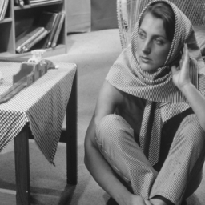
\includegraphics[width = 0.60\textwidth]{barbara_original256x256.png}
    \caption{}
    \label{subfig:barbara_original}
\end{subfigure}%
\begin{subfigure}{0.55\textwidth}
    \centering
    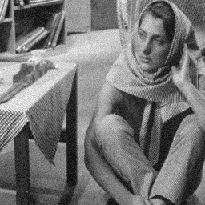
\includegraphics[width = 0.60\textwidth]{barbara_noisy_sigma=10_lambda=32.png}
    \caption{}
    \label{subfig:barbara_noisy}
\end{subfigure}

\begin{subfigure}{0.55\textwidth}
    \centering
    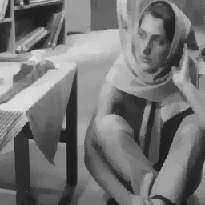
\includegraphics[width = 0.60\textwidth]{barbara_denoised_sigma=10_lambda=32_umap.png}
    \caption{}
    \label{subfig:barbara_umap}
\end{subfigure}%
\begin{subfigure}{0.55\textwidth}
    \centering
    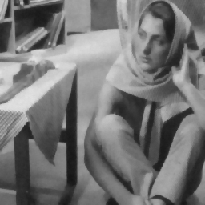
\includegraphics[width = 0.60\textwidth]{barbara_denoised_sigma=10_lambda=32_upm.png}
    \caption{}
    \label{subfig:barbara_upm}
\end{subfigure}
    \caption{The anisotropic ROF model endowed with 4-nearest neighbors is applied to the test image "Barbara". The original image is shown in (a). The image is corrupted by Gaussian noise (zero mean with standard deviation $\sigma = 10$) and is shown in (b). The corresponding minimizer $\bu_{MAP}(\bx,t)$ given by \eqref{eq:rof_model} and posterior mean estimate $\bu_{PM}(\bx,t,\epsilon)$ given by \eqref{eq:rof_model_pm} with parameters $t = 16$ and $\epsilon = 6.25$ are illustrated in (c) and (d), respectively.}
    \label{fig:barbara_images}
\end{figure}

\begin{figure}[ht]
    \centering
\begin{subfigure}{0.55\textwidth}
    \centering
    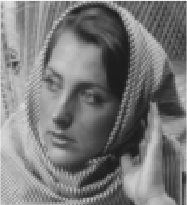
\includegraphics[width = 0.60\textwidth]{barbara_original256x256_zoom-in.png}
    \caption{}
    \label{subfig:barbara_zoom}
\end{subfigure}%
\begin{subfigure}{0.55\textwidth}
    \centering
    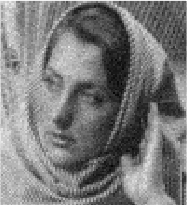
\includegraphics[width = 0.60\textwidth]{barbara_noisy_sigma=10_lambda=32_zoom-in.png}
    \caption{}
    \label{subfig:barbara_noisy_zoom}
\end{subfigure}

\begin{subfigure}{0.55\textwidth}
    \centering
    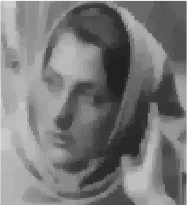
\includegraphics[width = 0.60\textwidth]{barbara_denoised_sigma=10_lambda=32_umap_zoom-in.png}
    \caption{}
    \label{subfig:barbara_umap_zoom}
\end{subfigure}%
\begin{subfigure}{0.55\textwidth}
    \centering
    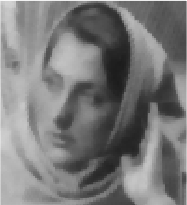
\includegraphics[width = 0.60\textwidth]{barbara_denoised_sigma=10_lambda=32_upm_zoom-in.png}
    \caption{}
    \label{subfig:barbara_upm_zoom}
\end{subfigure}
    \caption{The anisotropic ROF model endowed with 4-nearest neighbors is applied to the test image "Barbara". Images (a)-(d) are zoomed-in versions of the images illustrated in Figure~\ref{fig:barbara_images}.}
    \label{fig:zoomed-in_images}
\end{figure}

Variational methods are popular because the resultant optimization problem for various non-smooth and convex regularization terms used in image denoising problems, such as total variation and $l_1$-norm based regularization terms, is well-understood \cite{bouman1993generalized,candes2006robust,chambolle1997image,darbon2015convex,darbon2019decomposition,donoho2006compressed,rudin1992nonlinear} and can be solved efficiently using robust numerical optimization methods \cite{chambolle2016introduction}. MAP estimates from variational methods are also generally faster to compute than posterior mean estimates, the latter which require complex stochastic methods to compute. Reconstructed images from variational methods with non-smooth and convex regularization terms, however, may have undesirable and visually unpleasant staircasing effects due to the singularities of the non-smooth regularization terms \cite{chan2000high,dobson1996recovery,durand2000image,nikolova2007model,louchet2008modeles,woodford2009global}. This is illustrated for example in Figure 1(c), which contains regions where the pixel values are equal and lead to staircasing effects. In contrast, posterior mean estimates with quadratic fidelity term and total variation regularization terms have been shown to avoid staircasing effects \cite{louchet2008modeles,louchet2013posterior}. This is illustrated for example in Fig.~\ref{fig:barbara_images} and~\ref{fig:zoomed-in_images}(d), where the denoised image with posterior mean estimate does not contain visibly substantial regions where the pixel values are equal.

\bigbreak
\noindent
\textbf{Related work.} 
Several papers have proposed original connections between MAP and Bayesian estimators, including posterior mean estimators. First, \cite{louchet2008modeles,louchet2013posterior} showed that the class of Bayesian posterior mean estimates \eqref{eq:pm_estimate} with TV regularization term $J$ can be expressed as minimizers to optimization problems involving a quadratic fidelity term and a smooth convex regularization term, i.e., there exists a smooth regularization term $f_{\rm{reg}}\colon \Rn \to \R$ such that
\begin{equation}\label{eq:pm_rep_map}
\bu_{PM}(\bx,t,\epsilon) = \argmin_{\by \in \Rn} \left\{\frac{1}{2}\normsq{\bx-\by} + f_{\rm{reg}}(\by)\right\}.
\end{equation}
This result was later extended to general priors \cite{gribonval2011should}, general Gaussian data fidelity terms \cite{gribonval2013reconciling}, and to some non-quadratic data fidelity terms \cite{gribonval2018bayesian,gribonval2018characterization}. To our knowledge, there is no representation formula for this smooth regularization term available in the literature. 

Second, \cite{burger2014maximum} showed that the MAP estimate~\eqref{eq:minimizer_prob} corresponds to a Bayes estimator when the regularization term $J$ is convex and uniformly Lipschitz continuous on $\Rn$, that is, the MAP estimate~\eqref{eq:minimizer_prob} minimizes the posterior expected value of an appropriate loss function. This was later extended by \cite{burger2016bregman} to some log-concave posterior distributions with non-quadratic fidelity term, and later studied from the point of view of differential geometry in \cite{pereyra2019revisiting} and also derived for posterior distributions that are strongly log-concave and at least three times differentiable.

In addition to these results, it is known that under certain assumptions on the regularization term $J$, the value of the minimization problem
\begin{equation} \label{eq:minimization_prob} 
S_{0}(\bx,t)\coloneqq\min_{\by\in\Rn}\left\{ \frac{1}{2t}\normsq{\bx-\by}+J(\by)\right\}
\end{equation}
whose minimizer is the MAP estimate~\eqref{eq:minimizer_prob}, satisfies the first-order HJ PDE 
\begin{equation}
\begin{dcases}
\frac{\partial S_0}{\partial t}(\bx,t)+\frac{1}{2}\normsq{\nabla_{\bx}S_0(\bx,t)}=0 & \mbox{in }\Rn\times(0,+\infty),\\
S_0(\bx,0)=J(\bx) & \mbox{in }\Rn.
\end{dcases}
\end{equation}
The properties of the minimizer $\bu_{MAP}(\bx,t)$ follow from the properties of the solution to this HJ equation~\cite{darbon2015convex,darbon2019decomposition}. In particular, the MAP estimate satisfies the representation formula $\bu_{PM}(\bx,t) = \bx - t\nabla_{\bx}S_0(\bx,t)$. 

We note that the results of \cite{darbon2015convex,darbon2019decomposition} considers only connections between a class of first-order HJ PDEs and MAP estimators. To our knowledge, connections between posterior estimators and HJ PDEs are not available in the literature.

\bigbreak
\noindent
\textbf{Contributions.} 
In this paper, we propose original connections between solutions to HJ PDEs and a broad class of Bayesian methods and posterior mean estimators. These connections are described in Prop.~\ref{thm:visc_hj_eqns} and~\ref{thm:char_opt_sol} for viscous HJ PDEs and first-order HJ PDEs, respectively. We show in Prop.~\ref{thm:visc_hj_eqns} that the posterior mean estimate~\eqref{eq:pm_estimate} is described by the solution to a viscous HJ with initial data corresponding to the convex regularization term $J$, which we characterize in detail in terms of the data $\bx$ and parameters $t$ and $\epsilon$. In particular, the posterior mean estimate~\eqref{eq:pm_estimate} satisfies the representation formula $\bu_{PM}(\bx,t,\epsilon) = \bx - t\nabla_{\bx}S_\epsilon(\bx,t)$. Next, we use the connections between viscous HJ PDEs and posterior mean estimates established in Prop.~\ref{thm:visc_hj_eqns} to show in Prop.~\ref{thm:char_opt_sol} that the posterior mean estimate $\bu_{PM}(\bx,t,\epsilon)$ can be expressed through the gradient of the solution to a first-order HJ PDE with twice continuously differentiable convex initial data $\Rn \ni \bx \mapsto K^{*}_{\epsilon}(\bx,t)-\frac{1}{2}\Vert \bx \Vert_{2}^{2}$, where
\[
K_{\epsilon}(\bx,t) = t\epsilon\ln\left(\frac{1}{(2\pi t\epsilon)^{n/2}}\int_{\dom J}e^{\left(\frac{1}{t}\left\langle \bx,\by\right\rangle -\frac{1}{2t}\left\Vert \by\right\Vert _{2}^{2}-J(\by)\right)/\epsilon}\diff\by\right)
\]
and $\bx \mapsto  K^{*}_{\epsilon}(\bx,t)$ is the Fenchel--Legendre transform of the function $\bx \mapsto K_{\epsilon}(\bx,t)$. In other words, we show
\[
\bu_{PM}(\bx,t,\epsilon) = \argmin_{\by \in \Rn}\left\{\frac{1}{2}\normsq{\bx-\by} + \left( K^{*}_{\epsilon}(\by,t)-\frac{1}{2}\Vert \by \Vert_{2}^{2}\right)\right\}.
\]
This formula gives the representation of the convex regularization term enabling one to express the posterior mean estimate as the minimizer of a convex variational problem, and in fact in terms of the solution to a first-order HJ PDE, thereby extending the results of \cite{louchet2008modeles,gribonval2011should} who showed existence of this regularization term when the data fidelity term is quadratic, but not its representation. The twice continuously differentiability of this regularization term, in particular, implies that the posterior mean estimate $\bu_{PM}(\bx,t,\epsilon)$ avoids image denoising staircasing effects as a consequence of the results derived in (\cite{nikolova2004weakly}, Theorem 3).

We also present several topological properties of posterior mean estimators in Proposition~\ref{prop:topo_properties} and we use these in conjunction with the connections between HJ PDEs and posterior mean estimators to derive representation and monotonicity properties of posterior mean estimators in Propositions~\ref{prop:pm_rep_props} and \ref{prop:mono_properties}, respectively. These properties are then used to derive an optimal upper bound on the mean squared error $\expectationJ{\normsq{\by-\bu_{PM}(\bx,t,\epsilon)}}$, an estimate of the squared difference between the MAP and posterior mean estimates, monotone and non-expansive properties of the posterior mean estimate, and the behavior of the posterior mean estimate $\bu_{PM}(\bx,t,\epsilon)$ in the limit $t \to 0$ (Proposition~\ref{prop:bounds_limits}). Finally, we use the connections between both MAP and posterior mean estimates and HJ PDEs to characterize the MAP estimate~\eqref{eq:minimizer_prob} in the context of Bayesian estimation theory, and specifically in Prop.~\ref{thm:bregman_div} to show that the MAP estimate~\eqref{eq:minimizer_prob} corresponds to the Bayes estimator of the Bayesian risk~\eqref{eq:breg2} whenever $J$ is convex on $\Rn$ and bounded from below. When $J$ is defined only on a strict subset of $\Rn$, we further show that the Bayesian risk~\eqref{eq:breg2} has a corresponding Bayes estimator that is described in terms of the solution to both the first-order HJ PDE~\eqref{thm:e_u_nonvisc_hj} and the viscous HJ PDE~\eqref{thm:visc_hj_eqns}.

\bigbreak
\noindent
\textbf{Organization.} 
In Section \ref{sec:background}, we review concepts of real and convex analysis that will be used throughout this paper. In Section~\ref{sec:connections}, we establish theoretical connections between a broad class of Bayesian posterior mean estimators and HJ PDEs. Our mathematical set-up is described in Subsection~\ref{subsec:set-up}, the connections of posterior mean estimators to viscous HJ PDEs are described in Subsection~\ref{subsec:HJ_eqns_visc}, and the connections of posterior mean estimators to first-order HJ PDEs are described in Subsection~\ref{subsec:HJ_eqns_1order}. We use these connections to establish various properties of posterior mean estimators in Section~\ref{sec:properties_estimators}. Specifically, we present topological, representation, and monotonicity properties of posterior mean estimators in Subsection~\ref{subsec:prop_topo-rep-mono}, an optimal upper bound on the mean squared error $\expectationJ{\normsq{\by-\bu_{PM}(\bx,t,\epsilon)}}$, an estimate of the squared difference between the MAP and posterior mean estimates, monotone and non-expansive properties of the posterior mean estimate, and the behavior of the posterior mean estimate $\bu_{PM}(\bx,t,\epsilon)$ in the limit $t \to 0$ in Subsection~\ref{subsec:prop_bounds-est}. Finally, we establish properties of MAP and posterior mean estimators in terms of Bayesian risks involving Bregman divergences in Subsection~\ref{subsec:prop_breg_div}.
\section{Background} \label{sec:background}
This section reviews concepts from real and convex analysis that will be used in this paper. We refer the reader to \cite{folland2013real,hiriart2013convexI,hiriart2013convexII,rockafellar1970convex,rockafellar2009variational} for comprehensive references. In what follows, the Euclidean scalar product on $\Rn$ will be denoted by $\left\langle \cdot,\cdot\right\rangle $ and its associated norm by $\left\Vert \cdot\right\Vert _{2}$. The closure and interior of a non-empty set $C\subset\Rn$ will be denoted by $\cl C$ and $\inter C$, respectively. The boundary of a non-empty set $C\subset\Rn$ is defined as $\cl C \setminus \inter C$ and will be denoted by $\bd C$. The domain of a function $f\colon\Rn\to\R\cup\{+\infty\}$ is the set $\dom f = \left\{ \bx\in\Rn : f(\bx)<+\infty\right\}$.
%
%
Let $f:\Omega \times \Omega' \to \R$ with $\Omega\times\Omega' \subset \Rn\times\mathbb{R}^{n'}$ at $(\bx,\by) \in \Omega\times \Omega'$. It will be useful in this paper to consider the gradient $\nabla_{\bx}f(\bx,\by)$, divergence $\nabla_{\bx} \cdot f(\bx,\by)$ and Laplacian $\Delta_{\bx} f(\bx,\by)$ of $\Omega \ni \bx \mapsto f(\bx,\by)$ for $\by \in \Omega'$, which are defined as follows: $\nabla_{\bx} f(\bx,\by) = \left(\frac{\partial f}{\partial x_1} (\bx,\by), \dots, \frac{\partial f}{\partial x_n} (\bx,\by)\right)$,
$\nabla_x \cdot f(\bx,\by) = \sum_{i=1}^n\frac{\partial f}{\partial x_i}(\bx,\by)$, and
$\Delta_x f(\bx,\by) = \sum_{i=1}^n\frac{\partial^2 f}{\partial x_i^2}(\bx,\by)$.

For convenience to the reader, we summarize some notations and definitions in Table~\ref{tab:definitions}; the definitions are explained in detail below.
\newcolumntype{s}{>{\hsize=.7\hsize}X}
\begin{table}[!h]
\centering
 \caption{Notation used in this paper. Here, we use $C$ to denote a set in $\R^n$, $f$ to denote a function from $\R^n$ to $\R\cup\{+\infty\}$ and $\bx$ to denote a vector in $\Rn$. The closure and interior of a non-empty set $C \subset \Rn$ are denoted by $\cl C$ and $\inter C$, respectively.} 
 \label{tab:definitions}
\begin{tabularx}{\textwidth}{ l|s|X }
\hline
\noalign{\smallskip}
 Notation & Meaning & Definition\\
 \noalign{\smallskip}
 \hline
 \noalign{\smallskip}
%
 $\left\langle \cdot,\cdot\right\rangle $ & 
 Euclidean scalar product in $\mathbb{R}^{n}$ & $\langle \bx, \by\rangle \coloneqq \sum_{i=1}^n x_iy_i$
 \\
 $\left\Vert \cdot\right\Vert _{2}$ &
 Euclidean norm in $\mathbb{R}^{n}$ & $\left\Vert \bx\right\Vert _{2} \coloneqq \sqrt{\langle \bx, \bx\rangle}$
 \\
 $\ri C$ & Relative interior of $C$ & The interior of $C$ with respect to the minimal hyperplane containing $C$ in $\Rn$
 \\
 $\bd C$ & Boundary of $C$ & The boundary of a non-empty set $C$ is defined as $\cl C \setminus \inter C$.
 \\
 $\dom f$ & Domain of $f$ & $\{\bx\in \Rn:\ f(\bx) < +\infty\}$
 \\
 $\gmRn$ & A useful and standard class of convex functions & The set containing all proper, convex, lower semicontinuous functions from $\Rn$ to $\R\cup\{+\infty\}$
 \\
 $\pi_{C}(\bx)$ & $\pi_{C}(\bx)\coloneqq\argmin_{\by\in C}\left\Vert \bx-\by\right\Vert _{2}^{2}$ & Projection of $\bx \in \Rn$ onto the closed convex set $C$.
 \\
 $\partial f(\bx)$ & Subdifferential of $f$ at $\bx$ & $\{\bp\in\Rn:\ f(\by)\geqslant f(\bx) + \langle \bp, \by-\bx\rangle \ \forall \by\in\Rn\}$
 \\
 $\dom \partial f$ & $\bx \in \dom \partial f \implies \partial f(\bx) \neq \varnothing$ & The set of points $\bx \in \dom f$ for which the subdifferential $\partial f(\bx)$ is non-empty.
 \\
 $f^*$ & Fenchel--Legendre transform of $f$ & $f^*(\bp) \coloneqq \sup_{\bx\in \Rn} \{\langle \bp, \bx\rangle - f(\bx)\}$
 \\
 \noalign{\smallskip}
\hline
 \end{tabularx}
\end{table}

\begin{defn}[Proper and lower semicontinuous functions] \label{def:domains_prop}
A function $f\colon\Rn\to\R\cup\{+\infty\}$ is proper if $\dom f \neq \varnothing$ and $f(\bx) > -\infty$ for every $\bx \in \dom f$. 

A function $f\colon\Rn\to\R\cup\{+\infty\}$ is lower semicontinuous at $\bx\in\Rn$ if it satisfies $\liminf_{k\to+\infty}f(\bx_{k})\geqslant f(\bx)$ for every sequence $\left\{ \bx_{k}\right\} _{k=1}^{+\infty}\subset\Rn$ such that $\lim_{k\to+\infty}\bx_{k}=\bx$.
\end{defn}
%
\begin{defn}[Convex sets and their relative interiors] \label{def:convex_sets}
A subset $C\subset\Rn$ is convex if for every pair $(\bx,\by) \in C \times C$ and every scalar $\lambda \in (0,1)$, the line segment $\lambda\bx+(1-\lambda)\by$ is contained in $C$.

The relative interior of a convex set $C$, denoted by $\ri(C)$, is the set of points in the interior of the unique smallest affine set containing $C$. Every convex set $C$ with non-empty interior is $n$-dimensional with $\ri C=\inter C$ and has positive Lebesgue measure, and furthermore the $n$-dimensional Lebesgue measure of the boundary $\bd C$ is equal to zero \cite{lang1986note}.
\end{defn}
%
\begin{defn}[Convex functions and the set $\gmRn$] \label{def:convex} 
A proper function $f\colon\Rn\to\R\cup\{+\infty\}$ is convex if its domain is convex and if the inequality
\[
f(\lambda\bx+(1-\lambda)\by)\leqslant\lambda f(\bx)+(1-\lambda)f(\by)
\]
holds for every pair $(\bx,\by) \in \dom f \times \dom f$ and every scalar $\lambda\in[0,1]$. It is \textit{strictly convex} if the inequality above is strict whenever $\bx\neq\by$ and $\lambda \in (0,1)$, and it is \textit{strongly convex with parameter $m>0$} if 
\[
f(\lambda\bx+(1-\lambda)\by)\leqslant\lambda f(\bx)+(1-\lambda)f(\by)-\frac{m}{2}\lambda(1-\lambda)\left\Vert \bx-\by\right\Vert _{2}^{2}
\]
for every pair $(\bx,\by) \in \dom f \times \dom f$ and every scalar $\lambda\in[0,1]$.

The class of proper, convex and lower semicontinuous functions is denoted by $\gmRn$.
\end{defn}
%
\begin{defn}[Projections] \label{def:projections} 
Let $C$ be a closed convex subset of $\Rn$. To every $\bx \in \Rn$, there exists a unique element $\pi_{C}(\bx) \in C$ called the projection of $\bx$ onto $C$ that is closest to $\bx$ in Euclidean norm, i.e.,
\begin{equation} \label{eq:proj_def}
\pi_{C}(\bx)\coloneqq\argmin_{\by\in C}\left\Vert \bx-\by\right\Vert _{2}^{2}.
\end{equation}
This correspondence defines a map $\bx \mapsto \pi_{C}(\bx)$ from $\Rn$ to $C$ called the projector onto $C$ (\cite{aubin2012differential}, Chapter 0.6, Corollary 1). It satisfies the characterization
\begin{equation} \label{eq:proj_char}
\left\langle \bx-\pi_{C}(\bx),\by-\pi_{C}(\bx)\right\rangle \leqslant0, \quad\forall\by\in C.
\end{equation}
\end{defn}
%
\begin{comment}
\begin{defn}[Differentiability and the gradient] \label{def:diff_grad}
Let $\Omega$ be an open set, $f\colon \Omega \to \R$, and $\bx \in \Omega$. The function $f$ is \textit{differentiable} at $\bx \in \Omega$ if there exists a linear form $Df(\bx) \colon \Rn\to\R$ such that
\[
f(\bx+\bh) = f(\bx) + Df(\bx) + o(\normtwo(\bh)),
\]
where $\lim_{\normtwo(\bh) \to 0}o(\normtwo(\bh)) = 0$.
The linear form $Df(\bx)$ is called the differential of $f$ at $\bx$, and it can be represented by a unique vector $\nabla f(\bx) \in \Rn$ via $Df(\bx)(\bh) = \left \langle \nabla f(\bx),\bh \right\rangle$ for every $\bh \in \Rn$. The element $\nabla f(\bx)$ is called the gradient of $f$ at $\bx$.
\end{defn}
\end{comment}
%
\begin{defn}[Subdifferentials and subgradients] \label{def:subgrad} 
Let $f \in \gmRn$. The \textit{subdifferential} of $f$ at $\bx\in\dom f$ is the set $\partial f(\bx)$ of vectors $\bp\in\Rn$ that satisfies the inequality
\begin{equation} \label{eq:subgrad_def}
f(\by)\geqslant f(\bx)+\left\langle \bp,\by-\bx\right\rangle
\end{equation}
for every $\by \in \Rn$. The subdifferential $\partial f(\bx)$ is a closed convex subset of $\Rn$ whenever it is non-empty, and the vectors $\bp\in\partial f(\bx)$ are called the subgradients of $f$ at $\bx$.

The set of points $\bx\in\dom f$ for which the subdifferential $\partial f(\bx)$ is non-empty is denoted by $\dom\partial f$, and it includes the relative interior of the domain of $f$, i.e., $\ri(\dom f) \subset \dom\partial f$ (\citep{rockafellar1970convex}, Theorem 23.4). 

If $f$ is strongly convex of parameter $m > 0$, then the subgradients of $f$ at $\bx \in \dom \partial f$ satisfy the following inequality
\[
f(\by)\geqslant f(\bx)+\left\langle \bp,\by-\bx\right\rangle + \frac{m}{2}\normsq{\by-\bx}.
\]

If $f$ is differentiable at $\bx$, then $\bx \in \dom\partial f$ and the gradient $\nabla f(\bx)$ is the unique subgradient of $f$ at $\bx$, and conversely if $f$ has a unique subgradient at $\bx$, then $f$ is differentiable at that point (\citep{rockafellar1970convex}, Theorem 25.1).

The set-valued subdifferential mapping $\dom \partial f \ni \by \mapsto \partial f(\by)$ satisfies two important properties. First, it is monotone in that if $f$ is strongly convex of parameter $m \geqslant 0$ for every pair $(\by,\by_{0}) \in \dom\partial f \times \dom\partial f$ and $\bp\in\partial f(\by)$, $\bp_{0}\in\partial f(\by_{0})$, the following inequality holds (\cite{rockafellar1970convex}, page 240 and Corollary 31.5.2):
\begin{equation} \label{eq:monotone_mapping}
m\normsq{\by-\by_0} \leqslant \left\langle \bp-\bp_{0},\by-\by_{0}\right\rangle.
\end{equation}
Second, the mapping $\dom\partial f \ni \by \mapsto \pi_{\partial f(\by)}(\boldsymbol{0})$ is well-defined, and it selects the subgradient of the minimal norm in $\partial f(\bx)$ and defines a function continuous almost everywhere on $\dom\partial f$, a consequence of the fact that this mapping agrees with the gradient of $f$ over the set of points in $\inter(\dom J)$ at which $f$ is differentiable (\cite{rockafellar1970convex}, Theorem 25.5). 
\end{defn}
%
\begin{defn}[Fenchel--Legendre transform] \label{def:legendre_t} 
Let $f\in\gmRn$. The \textit{Fenchel--Legendre transform} $f^{*}\colon\Rn\to\mathbb{R\cup}\{+\infty\}$ of $f$ is defined by
\begin{equation}
f^{*}(\bp)=\sup_{\bx\in\Rn}\left\{ \left\langle \bp,\bx\right\rangle -f(\bx)\right\} .\label{eq:fenchel_t_def}
\end{equation}
For every $f\in\gmRn$, the mapping $f\mapsto f^{*}$ is one-to-one, $f^{*}\in\gmRn$, and $(f^{*})^{*}=f$. Moreover, for every $\bx\in\Rn$ and $\bp\in\Rn$, $f$ and $f^*$ satisfy Fenchel's inequality
\begin{equation} \label{eq:fenchel_ineq}
f(\bx)+f(\bp)\geqslant\left\langle \bx,\bp\right\rangle,
\end{equation}
where equality holds if and only if $\bp\in\partial f(\bx)$, if and only if $\bx\in\partial f^{*}(\bp)$ (\citep{hiriart2013convexII}, corollary 1.4.4). If $f$ is also differentiable, the supremum in (\ref{eq:fenchel_t_def}) is attained whenever there exists $\bx\in\Rn$ such that $\bp=\nabla f(\bx)$. 
\end{defn}
%
\begin{defn}[Bregman divergences] \label{def:breg_div} 
Let $f\in\gmRn$. The \textit{Bregman divergence} of $f$ is the function $D_{f}\colon\Rn\times\Rn\to\R\cup\{+\infty\}$ defined by
\begin{equation}
D_{f}(\bx,\bp)=f(\bx)-\left\langle \bp,\bx\right\rangle +f^{*}(\bp).\label{eq:breg_good_def}
\end{equation}
It satisfies $D_{f}(\bx,\bp)\geqslant0$ for every $\bx\in\Rn$ and $\bp\in\Rn$ by Fenchel's inequality (\ref{eq:fenchel_ineq}), with $D_{f}(\bx,\bp)=0$ whenever $\bp\in\partial f(\bx)$. It also satisfies $D_{f}(\bx,\bp)=D_{f^{*}}(\bp,\bx)$, with $D_{f}(\bx,\bp)=D_{f}(\bp,\bx)$ if and only if $f$ is the quadratic $f=\frac{1}{2}\left\Vert \cdot\right\Vert _{2}^{2}$.
\end{defn}
%
\begin{defn}[Infimal convolutions] \label{def:inf_conv}
Let $f_{1}\in\gmRn$ and $f_{2}\in\gmRn$. The \textit{infimal convolution} of $f_{1}$ and $f_{2}$ is the function
\begin{equation}\label{eq:infconv_def}
\Rn \ni \bx \mapsto (f_{1} \Box f_{2})(\bx) = \inf_{\bx_{1}+\bx_{2}=\bx}\left\{ f_{1}(\bx_{1})+f_{2}(\bx_{2})\right\}.
\end{equation}
The infimal convolution is exact if the infimum is attained at $\bx_{1}\in\dom f_{1}$ and $\bx_{2}\in\dom f_{2}$, and in that case the infimum in \eqref{eq:infconv_def} can be replaced by a minimum. The Fenchel--Legendre transform of the infimal convolution (\ref{eq:infconv_def}) is the sum of their respective Fenchel--Legendre transforms (\citep{rockafellar1970convex}, Theorem 16.4), that is,
\[
\left(f_{1}\Box f_{2}\right)^{*}(\bp)=f_{1}^{*}(\bp)+f_{2}^{*}(\bp).
\]
%
If $f \in \gmRn$, then Moreau's decomposition Theorem \cite{hiriart1989moreau,moreau1965proximite} asserts that
\[
\frac{1}{2}\normsq{\cdot}\Box f + \frac{1}{2}\normsq{\cdot}\Box f^* = \frac{1}{2}\normsq{\cdot}.
\]
\end{defn}
%
The following proposition provides conditions for which two functions $f_1$ and $f_2$ satisfying $f_1 + f_2 = \frac{1}{2}\normsq{\cdot}$ can be factorized, respectively, in the form $\frac{1}{2}\normsq{\cdot}\Box f$ and $\frac{1}{2}\normsq{\cdot}\Box f^*$. The proof can be found in~\cite{hiriart1989moreau}.
\begin{prop}[Infimal deconvolutions \cite{hiriart1989moreau}] \label{prop:deconvolutions}
Suppose $f_1$ and $f_2$ are two convex functions on $\Rn$ such that $f_1 + f_2 = \frac{1}{2}\normsq{\cdot}$. Then there exists a unique function $f \in \gmRn$ such that
\[
f_1 = \frac{1}{2}\normsq{\cdot}\Box f\, \mbox{and }\, f_2 = \frac{1}{2}\normsq{\cdot}\Box f^*,
\]
where $f(\bx) = f_2^*(\bx) - \frac{1}{2}\normsq{\bx}$ for every $\bx \in \Rn$. Moreover, $f_1$ and $f_2$ are continuously differentiable and
\[
\nabla f_1(\bx)\in\partial f(\nabla h(\bx))\quad\mbox{and}\quad\nabla f_2(\bx)\in\partial f^{*}(\nabla g(\bx)).
\]
\end{prop}
%
\begin{defn}[Moreau--Yosida envelopes and proximal mappings]\label{def:moreau_yosida}
Let $t > 0$ and $J \in \gmRn$. The functions
\begin{equation}
\bx\mapsto \left(\frac{1}{2t}\|\cdot\|_2^2 \Box J\right)(\bx) \;=\;  \inf_{\by\in\Rn}\left\{ \frac{1}{2t}\normsq{\bx-\by}+J(\by)\right\} 
\end{equation}
and
\begin{equation}
\bx\mapsto \argmin_{\by\in\Rn}\left\{ \frac{1}{2t}\normsq{\bx-\by}+J(\by)\right\}
\end{equation}
are called the Moreau--Yosida envelope and proximal mapping of $J$, respectively \cite{hiriart2013convexII,moreau1965proximite,rockafellar2009variational}.
\end{defn}
%
The following proposition provides connections between HJ PDEs and Moreau--Yosida envelopes and proximal mappings, which corresponds to certain optimization problems in image denoising problems. Specifically, this proposition describes the behavior of the solution to the infimum problem \eqref{eq:minimization_prob} and its corresponding minimizer \eqref{eq:minimizer_prob}, and in particular that for any observed image $\bx\in\Rn$ and parameter $t>0$, the imaging problem \eqref{eq:minimization_prob} has always a unique solution. A summary of these results and their proof can be found in \cite{darbon2015convex}.
\begin{prop}[\cite{darbon2015convex}]\label{thm:e_u_nonvisc_hj}
Let $J\in\gmRn$. Then the following statements hold.
\begin{enumerate}
\item[(i)]  The unique continuously differentiable and convex function $S_0\colon\Rn\times[0,+\infty)\to\R$ that satisfies the first-order Hamilton--Jacobi equation with initial data
\begin{equation}
\begin{dcases}
\frac{\partial S_0}{\partial t}(\bx,t)+\frac{1}{2}\normsq{\nabla_{\bx}S_0(\bx,t)}=0 & \mbox{in }\Rn\times(0,+\infty),\\
S_0(\bx,0)=J(\bx) & \mbox{in }\Rn,
\end{dcases}\label{eq:hj_non_visc_pde}
\end{equation}
is defined by
\begin{align}
S_0(\bx,t) & = \left((\frac{1}{2t}\normsq{\cdot}) \Box J\right)(\bx) \qquad(\mbox{Lax--Oleinik formula}) \\
 & =\inf_{\by\in\Rn}\left\{ \frac{1}{2t}\normsq{\bx-\by}+J(\by)\right\}. \label{eq:lax_formula}
\end{align}
Furthermore, for every $\bx\in\dom J$, sequence $\{t_k\}_{k=1}^{+\infty}$ of positive real numbers converging to $0$, and sequence $\{\boldsymbol{d}_k\}_{k=1}^{+\infty}$ of vectors converging to $\boldsymbol{d}\in\Rn$, the pointwise limit $S_0(\bx+t_k\boldsymbol{d}_k,t_k)$ as $k \to +\infty$ exists and satisfies
\[
\lim_{k \to +\infty} S_0(\bx+t_k\boldsymbol{d}_k,t_k)=J(\bx).
\]
\item[(ii)]  For every $\bx\in\Rn$ and $t>0$, the infimum in (\ref{eq:lax_formula}) exists and is attained at a unique point $\bu_{MAP}(\bx,t)\in\dom\partial J$. In addition, the minimizer $\bu_{MAP}(\bx,t)$ satisfies the formula
\begin{equation} \label{eq:grad_map_rep}
\bu_{MAP}(\bx,t)=\bx-t\nabla_{\bx}S_0(\bx,t),
\end{equation}
and $\left(\frac{\bx-\bu_{MAP}(\bx,t)}{t}\right)\in\partial J(\bu_{MAP}(\bx,t))$.
\item[(iii)] Let $\{t_k\}_{k=1}^{+\infty}$ be a sequence of positive real numbers converging to zero and let $\{\boldsymbol{d}_k\}_{k=1}^{+\infty}$ be a sequence of elements in $\Rn$ converging to some $\boldsymbol{d} \in \Rn$. Then, for every $\bx \in \dom J$ the pointwise limit of $\bu_{MAP}(\bx,t)$ as $t\to0$ exists and satisfies
\[
\lim_{k\to +\infty} \bu_{MAP}(\bx + t_k\boldsymbol{d}_{k},t_k)=\bx.
\]
\item[(iv)] Let $\bx \in \dom\partial J$ and let $\{t_k\}_{k=1}^{+\infty}$ be a sequence of positive real numbers converging to zero. Then the limit of $\nabla_{\bx}S_0(\bx,t_k)$ as $k\to +\infty$ exists and satisfies
\begin{equation} \label{eq:grad_limit_subdiff}
    \lim_{k\to +\infty}\nabla_{\bx}S_0(\bx,t_k) = \pi_{\partial J(\by)}(\boldsymbol{0}).
\end{equation}
\end{enumerate}
\end{prop}
\section{Connections between Bayesian posterior mean estimators and Hamilton--Jacobi partial differential equations}  \label{sec:connections}

\subsection{Set-up} \label{subsec:set-up}
To establish connections between Bayesian posterior mean estimators and Hamilton--Jacobi equations, we will assume that the regularization term $J$ in the variational imaging model~\eqref{eq:minimization_prob} satisfies the following assumptions:
\begin{enumerate}
    \item[(A1)]  $J\in\gmRn$,
    \item[(A2)]  $\inter(\dom J)\neq \varnothing$,
    \item[(A3)]  $\inf_{\by\in\Rn}J(\by) \in \R$,
and without loss of generality, $\inf_{\by\in\Rn}J(\by)=0$.
\end{enumerate}
Assumption (A1) ensures that the minimal value of the convex imaging problem \eqref{eq:minimization_prob} and its minimizer \eqref{eq:minimizer_prob} are well-defined and enjoy several properties (see Section~\ref{sec:background}, Prop.~\ref{thm:e_u_nonvisc_hj}). Assumption (A2) ensures that for every $\bx \in \Rn$, $t>0$, and $\epsilon > 0$, the posterior distribution
\begin{equation} \label{eq:prob_dist_j}
    \Rn \ni \by \mapsto \frac{e^{-\left(\frac{1}{2t}\left\Vert \bx-\by\right\Vert _{2}^{2}+J(\by)\right)/\epsilon}}{\int_{\Rn}e^{-\left(\frac{1}{2t}\left\Vert \bx-\by\right\Vert _{2}^{2}+J(\by)\right)/\epsilon}\diff\by}
\end{equation}
and its associated partition function
\begin{equation} \label{eq:partition_function}
\Rn\times(0,+\infty)\times(0,+\infty)\ni(\bx,t,\epsilon)\mapsto Z_{J}(\bx,t,\epsilon)=\int_{\Rn}e^{-\left(\frac{1}{2t}\left\Vert \bx-\by\right\Vert _{2}^{2}+J(\by)\right)/\epsilon}\diff\by
\end{equation}
are well-defined, and finally, assumption (A3) guarantees that the partition function~\eqref{eq:partition_function} is also bounded from above independently of $\bx \in \Rn$. We will denote the posterior expectation (with respect to the posterior distribution~\eqref{eq:prob_dist_j}) of a measurable function $f\colon\Omega\mapsto\R$ with $\Omega\subset\dom f$ integrable on the set $\dom f \cap \dom J$ by
\begin{equation} \label{eq:expectation}
\expectationJ{f(\by)}=\frac{1}{Z_J(\bx,t,\epsilon)}\int_{\Omega \, \cap\, \dom J}f(\by)e^{-\left(\frac{1}{2t}\left\Vert \bx-\by\right\Vert _{2}^{2}+J(\by)\right)/\epsilon}\diff\by.
\end{equation}
Posterior expectations of vector quantities are defined similarly component-wise. Posterior expectations generally depends on $(x,t,\epsilon)$ but we will omit writing this dependence explicitly.

\subsection{Connections to viscous Hamilton--Jacobi partial differential equations} \label{subsec:HJ_eqns_visc}
The next proposition establishes connections between viscous HJ PDEs with initial data $J$ satisfying assumptions (A1)-(A3) and both the partition function~\eqref{eq:partition_function} and the Bayesian posterior mean estimate~\eqref{eq:pm_estimate}. These connections mirror those between the first-order HJ PDE~\eqref{eq:hj_non_visc_pde} with initial data $J$ satisfying assumption (A1) and both the convex minimization problem~\eqref{eq:minimization_prob} and the MAP estimate~\eqref{eq:minimizer_prob}. The connections between viscous HJ PDEs and Bayesian posterior mean estimators will be leveraged later to describe several properties of posterior mean estimators in terms of the observed image $\bx$ and parameters $t$ and $\epsilon$, and in particular in Section~\ref{subsec:HJ_eqns_1order} to show that the posterior mean estimate~\eqref{eq:pm_estimate} can be expressed as the minimizer associated to the solution to a first-order HJ PDE (Prop.~\ref{thm:char_opt_sol}) with at least twice continuously differentiable and convex regularization term.

\begin{prop}[The viscous Hamilton--Jacobi equation with initial data in $\gmRn$] \label{thm:visc_hj_eqns} Suppose the function $J$ satisfies assumptions (A1)-(A3). Then the following statements hold.
\begin{enumerate}
\item[(i)] (Cole--Hopf transformation, \cite{evans1998partial} Section 4.4.1) For every $\epsilon>0$, the function $S_\epsilon\colon\Rn\times[0,+\infty)\to[0,+\infty)$ defined by
\begin{equation} \label{eq:hj_s_eps}
S_{\epsilon}(\bx,t)\coloneqq-\epsilon\ln\left(\frac{1}{\left(2\pi t\epsilon\right)^{n/2}}Z_J(\bx,t,\epsilon)\right)=-\epsilon\ln\left(\frac{1}{\left(2\pi t\epsilon\right)^{n/2}}\int_{\Rn}e^{-\left(\frac{1}{2t}\left\Vert \bx-\by\right\Vert _{2}^{2}+J(\by)\right)/\epsilon}\diff\by\right)
\end{equation}
is the unique smooth solution to the viscous HJ PDE with initial data
\begin{equation}
\begin{dcases}\label{eq:hj_visc_pde}
\frac{\partial S_{\epsilon}}{\partial t}(\bx,t)+\frac{1}{2}\left\Vert \nabla_{\bx}S_{\epsilon}(\bx,t)\right\Vert _{2}^{2}=\frac{\epsilon}{2}\Laplacian S_{\epsilon}(\bx,t) & \text{ in }\Rn\times(0,+\infty),\\
S_{\epsilon}(\bx,0)=J(\bx) & \text{ in }\Rn.
\end{dcases}
\end{equation}
In addition, the domain of integration in \eqref{thm:visc_hj_eqns} can be taken to be $\dom J$ or, up to a set of Lebesgue measure zero, $\inter(\dom J)$ or $\dom(\partial J)$. Furthermore, for every $\bx\in\dom J$ and $\epsilon > 0$, except possibly at the boundary points $\bx\in(\dom J)\setminus\inter(\dom J)$ if such points exist, the pointwise limit $S_\epsilon(\bx,t)$ as $t \to 0$ exists and satisfies 
\begin{equation}
    \lim_{\substack{t\to0\\t>0}}S_{\epsilon}(\bx,t)=J(\bx).
\end{equation}
If $\bx\in(\dom J)\setminus\inter(\dom J)$, then we may only conclude 
\[
\liminf_{\substack{t\to0\\t>0}}S_{\epsilon}(\bx,t)\geqslant J(\bx)
\]
 and 
\[\limsup_{\substack{t\to0\\t>0}}S_{\epsilon}(\bx,t)\leqslant J(\bx)-\epsilon\ln\left(\frac{1}{(2\pi\epsilon)^{n/2}}\int_{\dom J}e^{-\frac{1}{2\epsilon}\left\Vert \bx-\by\right\Vert _{2}^{2}}\diff\by\right).
\]

\item[(ii)]  (Convexity and monotonicity properties).
\begin{enumerate}
    \item The function $\Rn\times(0,+\infty)\ni(\bx,t)\mapsto S_{\epsilon}(\bx,t)-\frac{n\epsilon}{2}\ln t$ is jointly convex.
    \item The function $(0,+\infty)\ni t\mapsto S_{\epsilon}(\bx,t)-\frac{n\epsilon}{2}\ln t$ is strictly monotone decreasing.
    \item The function $(0,+\infty)\ni\epsilon\mapsto S_{\epsilon}(\bx,t)-\frac{n\epsilon}{2}\ln\epsilon$ is strictly monotone decreasing.
    \item The function $\Rn \ni \bx \mapsto \frac{1}{2}\normsq{\bx} - tS_\epsilon(\bx,t)$ is strictly convex.
\end{enumerate}

\item[(iii)] (Connections to the posterior mean and mean squared error) The posterior mean estimate $\bu_{PM}(\bx,t,\epsilon)$ and the mean squared error $\expectationJ{\left \Vert \by - \bu_{PM}(\bx,t,\epsilon) \right \Vert_{2}^{2}}$ satisfy the formulas
\begin{equation} \label{eq:grad_s_eps}
    \bu_{PM}(\bx,t,\epsilon) = \bx - t\nabla_{\bx}S_\epsilon(\bx,t)
\end{equation}
and
\begin{equation}\label{eq:exact_variance}
\begin{alignedat}{1}
    \expectationJ{\left \Vert \by - \bu_{PM}(\bx,t,\epsilon) \right \Vert_{2}^{2}} &= t\epsilon \nabla_{\bx}\cdot \bu_{PM}(\bx,t,\epsilon) \\
    &= nt\epsilon - t^2\epsilon\Laplacian S_{\epsilon}(\bx,t).
\end{alignedat}
\end{equation}
Moreover, $\bx \mapsto \bu_{PM}(\bx,t,\epsilon)$ is a bijective function.

\item[(iv)] (Vanishing $\epsilon \to 0$ limit) Let $S_0:\Rn \times (0,+\infty) \to \R$ denote the continuously differentiable and convex solution to the first-order HJ PDE~\eqref{eq:hj_non_visc_pde} with initial data $J$. For every $\bx\in\Rn$ and $t>0$, the following limit holds:
\begin{equation} \label{eq:ldp_limit}
\lim_{\substack{\epsilon\to0\\\epsilon>0}} -\epsilon\ln\left(\frac{1}{\left(2\pi t\epsilon\right)^{n/2}}\int_{\Rn}e^{-\left(\frac{1}{2t}\left\Vert \bx-\by\right\Vert _{2}^{2}+J(\by)\right)/\epsilon}\diff\by\right) = \inf_{\by\in\Rn}\left\{ \frac{1}{2t}\left\Vert \bx-\by\right\Vert _{2}^{2}+J(\by)\right\},
\end{equation}
that is,
\[
\lim_{\substack{\epsilon\to0\\\epsilon>0}}S_{\epsilon}(\bx,t) = S_0(\bx,t),
\]
and the limit converges uniformly over every compact set of $\Rn\times(0,+\infty)$ in $(\bx,t)$. In addition, the gradient $\nabla_{\bx}S_{\epsilon}(\bx,t)$, the partial derivative $\frac{\partial S_{\epsilon}(\bx,t)}{\partial t}$, and the Laplacian $\frac{\epsilon}{2}\Laplacian S_{\epsilon}(\bx,t)$ satisfy the limits
\[
\lim_{\substack{\epsilon\to0\\\epsilon>0}}\nabla_{\bx}S_{\epsilon}(\bx,t)=\nabla_{\bx}S_0(\bx,t), \quad\lim_{\substack{\epsilon\to0\\
\epsilon>0}}\frac{\partial S_{\epsilon}}{\partial t}(\bx,t)=\frac{\partial S_0}{\partial t}(\bx,t),
\]
and
\[
\lim_{\substack{\epsilon\to0\\
\epsilon>0}}\frac{\epsilon}{2}\Laplacian S_{\epsilon}(\bx,t)=0,
\]
where each limit converges uniformly over every compact set of $\Rn\times(0,+\infty)$ in $(\bx,t)$. As a consequence, for every $\bx\in\Rn$ and $t>0$, the pointwise limit of $\bu_{PM}(\bx,t,\epsilon)$ as $\epsilon\to 0$ exists and satisfy
\[
\lim_{\substack{\epsilon\to0\\\epsilon>0}} \bu_{PM}(\bx,t,\epsilon) = \bu_{MAP}(\bx,t),
\]
and the limit converges uniformly over every compact set of $\Rn\times(0,+\infty)$ in $(\bx,t)$.
\end{enumerate}
\end{prop}

\begin{proof}
See Appendix~\ref{app:A}.
\end{proof}

To illustrate certain aspects of Prop.~\ref{thm:visc_hj_eqns} and properties of posterior mean estimates, we give here two analytical examples.

\begin{example}[Tikhonov--Phillips regularization] \label{example:tikhonov}
Let $J(\bx) = \frac{m}{2}\left \Vert \bx \right \Vert_{2}^{2}$ with $m>0$, and consider the solution $S_0(\bx,t)$ and $S_{\epsilon}(\bx,t)$ to the first-order PDE \eqref{eq:hj_non_visc_pde} and viscous HJ PDE \eqref{eq:hj_visc_pde} with initial data $J$, respectively. 

The solution $S_0(\bx,t)$ is given by the Lax--Oleinik formula (Prop.~\ref{thm:e_u_nonvisc_hj}, Eq.~\eqref{eq:lax_formula})
\begin{alignat*}{1}
S_0(\bx,t) & =\inf_{\by\in\Rn}\left\{ \frac{1}{2t}\left\Vert \bx-\by\right\Vert _{2}^{2}+\frac{m}{2}\left\Vert \by\right\Vert _{2}^{2}\right\} \\
& =\frac{m\left\Vert \bx\right\Vert _{2}^{2}}{2(1+mt)}.
\end{alignat*}
This minimization problem is a special case of Tikhonov--Phillips regularization (also known as ridge regression in statistics), a method for regularizing ill-posed problems in inverse problems and statistics using a quadratic regularization term \cite{phillips1962technique,tikhonov1995numerical}. The corresponding minimizer can be computed using the gradient $\nabla_{\bx}S_0(\bx,t)$ via equation \eqref{eq:grad_map_rep} in Prop.~\ref{thm:visc_hj_eqns}:
\begin{equation*}
\bu_{MAP}(\bx,t)  = \bx - t\nabla_{\bx}S_0(\bx,t) = \bx - \frac{mt\bx}{1+mt} = \frac{\bx}{1+mt}.
\end{equation*}

The solution $S_\epsilon(\bx,t)$ is given by the integral
\begin{alignat*}{1}
S_{\epsilon}(\bx,t) & =-\epsilon\ln\left(\frac{1}{(2\pi t\epsilon)^{n/2}}\int_{\Rn}e^{-\left(\frac{1}{2t}\left\Vert \bx-\by\right\Vert _{2}^{2}+\frac{m}{2}\left\Vert \by\right\Vert _{2}^{2}\right)/\epsilon}\diff\by\right)\\
 & =\frac{m\left\Vert \bx\right\Vert ^{2}}{2(1+mt)}+\frac{n\epsilon}{2}\ln\left(1+mt\right).
\end{alignat*}
The posterior mean estimate $\bu_{PM}(\bx,t,\epsilon)$ can be computed using the representation formula~\eqref{eq:grad_s_eps} in Prop.~\ref{thm:visc_hj_eqns}(iii) by calculating the gradient $\nabla_{\bx}S_\epsilon(\bx,t)$:
\begin{equation*}
\bu_{PM}(\bx,t,\epsilon)  = \bx - t\nabla_{\bx}S_\epsilon(\bx,t) = \bx - \frac{mt\bx}{1+mt} = \frac{\bx}{1+mt}.
\end{equation*}
The mean squared error $\expectationJ{\normsq{\by-\bu_{PM}(\bx,t,\epsilon)}}$ can be computed using the representation formula~\eqref{eq:exact_variance} in Prop.~\ref{thm:visc_hj_eqns}(iii) by calculating the divergence of $\bu_{PM}(\bx,t,\epsilon)$:
\begin{equation}\label{eq:tikhonov_var}
    \expectationJ{\left \Vert \by - \bu_{PM}(\bx,t,\epsilon)\right \Vert_{2}^{2}} = t\epsilon \nabla_{\bx} \cdot \bu_{PM}(\bx,t,\epsilon) = \frac{nt\epsilon}{1+mt}.
\end{equation}

Comparing the solutions $S_0(\bx,t)$ and $S_\epsilon(\bx,t)$, we see that $\lim_{\substack{\epsilon\to0\\
\epsilon>0}}S_{\epsilon}(\bx,t)=S_0(\bx,t)$ for every $\bx\in\Rn$ and $t>0$, in accordance to the result established in Prop.~\ref{thm:visc_hj_eqns}(iv). Note also that while $(\bx,t)\mapsto S_0(\bx,t)$ is jointly convex, its viscous counterpart $(\bx,t)\mapsto S_\epsilon(\bx,t)$ is not. Indeed, $t \mapsto S_\epsilon(\bx,t)$ is not convex, and it is convex only after subtracting $\frac{n\epsilon}{2}\ln t$ from $S_{\epsilon}(\bx,t)$.
\end{example}

\begin{example}[Soft thresholding] \label{ex:smooth_shrink} 
Let $J(\bx)=\sum_{i=1}^{n}\lambda_{i}\left|\bx_{i}\right|$, where $\lambda_{i}>0$ for each $i\in\{1,\dots,n\}$, and consider the solutions $S_0(\bx,t)$ and $S_{\epsilon}(\bx,t)$ to the first-order \eqref{eq:hj_non_visc_pde} and viscous HJ PDEs \eqref{eq:hj_visc_pde} with initial data $J$, respectively.

The solution $S_0(\bx,t)$ is given by the Lax--Oleinik formula
\begin{align*}
S_{0}(\bx,t) & =\inf_{\by\in\Rn}\left\{ \frac{1}{2t}\left\Vert \bx-\by\right\Vert _{2}^{2}+\sum_{i=1}^{n}\lambda_{i}\left|y_{i}\right|\right\} \label{eq:ex_sol_eps_0}\\
 & =\sum_{i=1}^{n}\left(\inf_{y_{i}\in\R}\left\{ \frac{1}{2t}(x_{i}-y_{i})^{2}+\lambda_{i}\left|y_{i}\right|\right\} \right),
\end{align*}
where $x_i$ and $y_i$ denote the $i^{\rm th}$ component of the vectors $\bx$ and $\by$, respectively. In the context of imaging, this minimization problem corresponds to denoising an image with the weighted sum of a quadratic fidelity term and a weighted $l_{1}$-norm as the regularization term. This term is widely used in imaging to encourage sparsity of an image, and it has received considerable interest due to its connection with compressed sensing reconstruction \citep{candes2006robust,donoho2006compressed}. The solution to this minimization problem corresponds to a soft thresholding applied component-wise to the vector $\bx$ \cite{daubechies2004iterative, figueiredo2001wavelet,lions1979splitting}. The soft thresholding operator is defined for any real number $a$ and positive real number $\alpha$ as
\begin{equation} \label{eq:thresholding_operator}
\R \times (0,+\infty) \ni (a,\alpha) \mapsto T(a,\alpha)=\begin{cases}
a-\alpha & \mbox{if }a>\alpha,\\
0 & \mbox{if }a\in[-\alpha,\alpha],\\
a+\alpha & \mbox{if }a<-\alpha.
\end{cases}
\end{equation}
The minimizer in the Lax--Oleinik formula of $S_0(\bx,t)$ is then given component-wise for $i\in\{1,\dots,n\}$ by
\[
\left(\bu_{MAP}(\bx,t)\right)_{i}=T(x_{i},t\lambda_{i}),
\]
so that
\begin{equation*}
S_{0}(\bx,t) = \sum_{i=1}^{n}\left( \frac{1}{2t}(x_{i}-T(x_{i},t\lambda_{i}))^{2}+\lambda_{i}\left|T(x_{i},t\lambda_{i})\right|\right).
\end{equation*}

The solution $S_\epsilon(\bx,t)$ is given by the integral
\begin{align*}
S_{\epsilon}(\bx,t) & =-\epsilon\ln\left(\frac{1}{(2\pi t\epsilon)^{n/2}}\int_{\Rn}e^{-\left(\frac{1}{2t}\left\Vert \bx-\by\right\Vert _{2}^{2}+\sum_{k=1}^{n}\lambda_{i}\left|y_{i}\right|\right)/\epsilon}\diff\by\right)\\
 & =-\epsilon\sum_{i=1}^{n}\ln\left(\frac{1}{2}\sqrt{\frac{2}{\pi t\epsilon}}\int_{-\infty}^{+\infty}e^{-\left(\frac{1}{2t}(x_{i}-y_i)^{2}+\lambda_{i}\left|y_i\right|\right)/\epsilon}\diff y_i\right)\\
 & =-\epsilon\sum_{i=1}^{n}\ln\left(\frac{1}{2}\sqrt{\frac{2}{\pi t\epsilon}}\left(\int_{0}^{+\infty}e^{-\left(\frac{1}{2t}(x_{i}+y_i)^{2}+\lambda_{i}y_i\right)/\epsilon}\diff y_i + \int_{0}^{+\infty}e^{-\left(\frac{1}{2t}(x_{i}-y_i)^{2}+\lambda_{i}y_i\right)/\epsilon}\diff y_i\right)\right)
\end{align*}
To compute this integral, first define the function
\begin{equation*}
    \R \ni z \mapsto L(z) = \frac{1}{2}e^{z^2}\erfc\left(z\right),
\end{equation*}
where $\erfc$ denotes the complementary error function. Then we have (\citep{gradshte2007table}, page 336, integral 3.332, 2., and page 887, integral 8.250, 1.)
\begin{equation*}
    \frac{1}{2}\sqrt{\frac{2}{\pi t\epsilon}}\int_{0}^{+\infty}e^{-\left(\frac{1}{2t}(x_{i}+y_i)^{2}+\lambda_{i}y_i\right)/\epsilon}\diff y_i = e^{-\frac{x_{i}^2}{2t\epsilon}}L\left(\frac{x_i + t\lambda_i}{\sqrt{2t\epsilon}}\right)
\end{equation*}
and
\begin{equation*}
    \frac{1}{2}\sqrt{\frac{2}{\pi t\epsilon}}\int_{0}^{+\infty}e^{-\left(\frac{1}{2t}(x_{i}-y_i)^{2}+\lambda_{i}y_i\right)/\epsilon}\diff y_i = e^{-\frac{x_{i}^2}{2t\epsilon}}L\left(\frac{-x_i + t\lambda_i}{\sqrt{2t\epsilon}}\right),
\end{equation*}
from which we get
\begin{equation*}
S_{\epsilon}(\bx,t)=\frac{\left\Vert \bx\right\Vert _{2}^{2}}{2t} -\epsilon\sum_{i=1}^{n}\ln\left(L\left(\frac{x_i + t\lambda_i}{\sqrt{2t\epsilon}}\right) + L\left(\frac{-x_i + t\lambda_i}{\sqrt{2t\epsilon}}\right)\right).
\end{equation*}
Now, to compute the posterior mean estimate it suffices to compute the gradient of $\nabla_{\bx}S_\epsilon(\bx,t)$ and use the formula $\bu_{PM}(\bx,t,\epsilon) = \bx - t\nabla_{\bx}S_\epsilon(\bx,t)$. To do so, we must compute the derivative of the function $L$. Since 
\begin{equation*}
    \frac{dL}{dz}(z) = 2zL(z)+\frac{1}{\sqrt{\pi}},
\end{equation*}
the chain rule gives 
\begin{equation*}
    \frac{\partial}{\partial x_i}\left(L\left(\frac{x_i + t\lambda_i}{\sqrt{2t\epsilon}}\right) + L\left(\frac{-x_i + t\lambda_i}{\sqrt{2t\epsilon}}\right)\right)  = \left(\frac{x_i + t\lambda_i}{t\epsilon}\right)L\left(\frac{x_i + t\lambda_i}{\sqrt{2t\epsilon}}\right) - \left(\frac{-x_i + t\lambda_i}{t\epsilon}\right)L\left(\frac{-x_i + t\lambda_i}{\sqrt{2t\epsilon}}\right).
\end{equation*}
The posterior mean estimate is therefore given component-wise by
\begin{alignat*}{1}
    (\bu_{PM}(\bx,t,\epsilon))_{i} & = x_i - t(\nabla_{\bx}S_\epsilon(\bx,t))_i\\
    & = x_i + t\lambda_i\left(\frac{L\left(\frac{x_i + t\lambda_i}{\sqrt{2t\epsilon}}\right) + L\left(\frac{-x_i + t\lambda_i}{\sqrt{2t\epsilon}}\right)}{L\left(\frac{x_i + t\lambda_i}{\sqrt{2t\epsilon}}\right) - L\left(\frac{-x_i + t\lambda_i}{\sqrt{2t\epsilon}}\right)}\right)
\end{alignat*}

The posterior mean estimate $\bu_{PM}(\bx,t,\epsilon)$ yields a smooth analogue of the soft thresholding operator $T$ (defined in \eqref{eq:thresholding_operator}) evaluated at $(x_i,t\lambda_i)$, in the sense that $\lim_{\substack{\epsilon\to0\\\epsilon>0}} (\bu_{PM}(\bx,t,\epsilon))_i = T(x_{i},t\lambda_{i})$ for every $i\in\{1,\dots,n\}$ by Prop.~\ref{thm:visc_hj_eqns}(iv). Figure~\ref{fig:sparsity_example} shows the MAP and posterior mean estimates in one dimension for the choice of $t=1.25$, $\epsilon=\left\{ 0.025,\,0.1,\,0.25,\,0.5,\,1\right\} $, and $\lambda_{1}=2$ for $x\in[-5,5]$.
\begin{figure}[h]
\centering
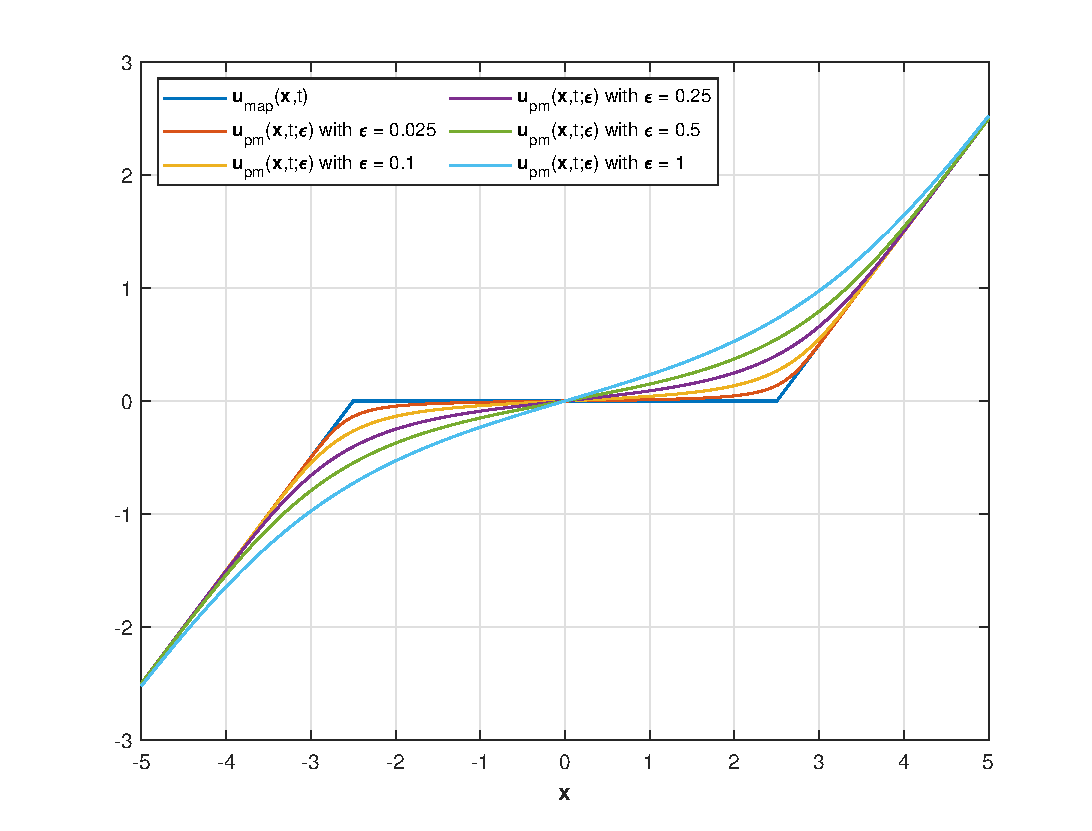
\includegraphics[width=0.75\textwidth]{u_pm_example_figure.pdf}
\caption{Numerical example of the MAP and posterior mean estimates in one dimension with $J(x)=\lambda_{1}\left|x\right|$ for the choice of $t=1.25$, $\epsilon=\left\{ 0.025,\,0.1,\,0.25,\,0.5,\,1\right\}$, and $\lambda_{1}=2$ for $x\in[-5,5]$.}
\label{fig:sparsity_example}
\end{figure}
\end{example}

\subsection{Connections to first-order Hamilton--Jacobi equations} \label{subsec:HJ_eqns_1order}

In this section, we use the connections between the posterior mean estimate~\eqref{eq:pm_estimate} and viscous HJ PDEs established in Prop.~\ref{thm:visc_hj_eqns} to show that the posterior mean estimate can be expressed through the solution to a first-order HJ PDE with initial data of the form of~\eqref{eq:hj_non_visc_pde}. In particular, we show that the posterior mean estimate satisfies the proximal mapping formula
\begin{equation*}
\bu_{PM}(\bx,t,\epsilon) = \argmin_{\by\in\Rn}\left\{ \frac{1}{2}\left\Vert \bx-\by\right\Vert _{2}^{2} + \left(K^{*}_{\epsilon}(\by,t)-\frac{1}{2}\Vert \by \Vert_{2}^{2}\right)\right\},
\end{equation*}
where the function $K_\epsilon\colon\Rn\times\times(0,+\infty) \to \R$ is defined through the solution $S_\epsilon(\bx,t)$ to the viscous HJ PDE~\eqref{eq:hj_visc_pde} via
\begin{equation*}
K_{\epsilon}(\bx,t) \coloneqq \frac{1}{2}\left\Vert \bx\right\Vert _{2}^{2}-tS_{\epsilon}(\bx,t) \equiv t\epsilon\ln\left(\frac{1}{(2\pi t\epsilon)^{n/2}}\int_{\dom J}e^{\left(\frac{1}{t}\left\langle \bx,\by\right\rangle -\frac{1}{2t}\left\Vert \by\right\Vert _{2}^{2}-J(\by)\right)/\epsilon}\diff\by\right),
\end{equation*}
which is convex by Prop.~\ref{thm:visc_hj_eqns}(ii)(d), and where $K^{*}_{\epsilon}(\by,t)$ denotes the Fenchel--Legendre transform of $\by \mapsto K_\epsilon(\by,t)$. This result gives the representation of the convex imaging regularization term whose existence was derived by \cite{louchet2008modeles,gribonval2011should,gribonval2013reconciling,louchet2013posterior} (and later extended to non-quadratic data fidelity terms in \cite{gribonval2018characterization,gribonval2018bayesian}). This representation result depends crucially on the connections established between the posterior mean estimate $\bu_{PM}(\bx,t,\epsilon)$ and the viscous HJ PDE~\eqref{eq:hj_visc_pde} established in Prop.~\ref{thm:visc_hj_eqns}. Moreover, we also show that $\by \mapsto K^{*}_{\epsilon}(\by,t)$ is at least twice continuously differentiable. This fact implies that the posterior mean estimate $\bu_{PM}(\bx,t,\epsilon)$ for image denoising does not suffer from staircasing effects thanks to a result established in (\cite{nikolova2004weakly}, Theorem 3) as proven for Total Variation regularization terms in \cite{louchet2008modeles}. Here, our results are applicable to any regularization term $J$ satisfying assumptions (A1)-(A3).

\begin{prop}[Connections between the posterior mean estimate and first-order HJ PDEs] \label{thm:char_opt_sol}
Suppose the function $J$ satisfies assumptions (A1)-(A3). For every $\bx \in \Rn$, $t>0$, and $\epsilon>0$, let $S_\epsilon(\bx,t)$ denote the solution to the viscous HJ PDE \eqref{eq:hj_visc_pde} with initial data $J$ and let $\bu_{PM}(\bx,t,\epsilon)$ denote the posterior mean estimate \eqref{eq:pm_estimate}. Consider the first-order HJ PDE
\begin{equation} \label{eq:hj_pde_mod}
\begin{dcases}
\frac{\partial\tilde{S}}{\partial s}(\bx,s)+\frac{1}{2}\left\Vert \nabla_{\bx}\tilde{S}(\bx,s)\right\Vert _{2}^{2}=0 & \textrm{\text{ in }}\,\Rn\times(0,+\infty),\\
\tilde{S}(\bx,0)=K^{*}_{\epsilon}(\bx,t)-\frac{1}{2}\Vert \bx \Vert_{2}^{2} & \textrm{\text{ in }}\,\Rn.
\end{dcases}
\end{equation}
Then the initial data $\bx \mapsto K^{*}_{\epsilon}(\bx,t)-\frac{1}{2}\Vert \bx \Vert_{2}^{2}$ is convex, the solution to the HJ PDE~\eqref{eq:hj_pde_mod} satisfies the Lax--Oleinik formula
\begin{equation*}
\tilde{S}(\bx,s) = \inf_{\by\in\Rn}\left\{ \frac{1}{2s}\left\Vert \bx-\by\right\Vert _{2}^{2} + \left(K^{*}_{\epsilon}(\by,t)-\frac{1}{2}\Vert \by \Vert_{2}^{2}\right)\right\},
\end{equation*}
and the corresponding minimizer at $s = 1$ is the posterior mean estimate $\bu_{PM}(\bx,t,\epsilon)$:
\begin{equation}\label{eq:upm_rep_map_est}
\bu_{PM}(\bx,t,\epsilon) = \argmin_{\by\in\Rn}\left\{ \frac{1}{2}\left\Vert \bx-\by\right\Vert _{2}^{2} + \left(K^{*}_{\epsilon}(\by,t)-\frac{1}{2}\Vert \by \Vert_{2}^{2}\right)\right\}.
\end{equation}
\end{prop}
Moreover, for every $t>0$ and $\epsilon > 0$ the function $\Rn \ni \by \mapsto K^{*}_{\epsilon}(\by,t)$ is at least twice continuously differentiable.

\begin{proof}
By definition of the function $(\bx,t) \mapsto K_{\epsilon}(\bx,t)$, we can write
\begin{equation*}
    tS_\epsilon(\bx,t) + K_\epsilon(\bx,t) = \frac{1}{2}\Vert \bx \Vert_{2}^{2}.
\end{equation*}
As both $\bx \mapsto tS_\epsilon(\bx,t)$ and $\bx \mapsto K_\epsilon(\bx,t)$ are convex by Prop.~\ref{thm:visc_hj_eqns}(ii)(a) and (d), we can apply Prop.~\ref{prop:deconvolutions} in Section~\ref{sec:background} to conclude that $\bx \mapsto K^{*}_{\epsilon}(\bx,t)-\frac{1}{2}\Vert \bx \Vert_{2}^{2}$ is convex and to express $tS_\epsilon(\bx,t)$ as
\begin{equation} \label{eq:s_eps_equiv}
    tS_\epsilon(\bx,t) = \inf_{\by \in \Rn}\left\{\frac{1}{2}\left \Vert \bx - \by \right \Vert_{2}^{2} + \left(K^{*}_{\epsilon}(\by,t) - \frac{1}{2}\left \Vert \by \right \Vert_{2}^{2}\right)\right\}
\end{equation}
On the one hand, by Prop.~\ref{thm:e_u_nonvisc_hj} the right hand side of \eqref{eq:s_eps_equiv} is the solution $\tilde{S}_0(\bx,s)$ to the first-order HJ PDE \eqref{eq:hj_pde_mod} at $s = 1$, and therefore its minimizer is given by $\bx - \nabla_{\bx}\tilde{S}_0(\bx,1)$. On the other hand, the gradient $\nabla_{\bx}\tilde{S}_0(\bx,1)$ is equal to the left hand side of \eqref{eq:s_eps_equiv}, that is, $\nabla_{\bx}\tilde{S}_0(\bx,1) = t\nabla_{\bx}S_\epsilon(\bx,t)$, which is equal to $\bx - \bu_{PM}(\bx,t,\epsilon)$ by formula~\eqref{eq:pm_estimate}. As a result, the posterior mean estimate $\bu_{PM}(\bx,t,\epsilon)$ minimizes the right hand side of \eqref{eq:s_eps_equiv}, that is, 
\begin{equation*}
\bu_{PM}(\bx,t,\epsilon) = \argmin_{\by\in\Rn}\left\{ \frac{1}{2}\left\Vert \bx-\by\right\Vert _{2}^{2} + \left(K^{*}_{\epsilon}(\by,t)-\frac{1}{2}\Vert \by \Vert_{2}^{2}\right)\right\}.
\end{equation*}

Now, using the strict convexity of $\bx \mapsto K_{\epsilon}(\bx,t)$ and that $\nabla K_\epsilon(\bx,t) = \bu_{PM}(\bx,t,\epsilon)$ is a bijective function in $\bx$ for every $t>0$ and $\epsilon>0$ by Prop.~\ref{thm:visc_hj_eqns}(iii) we can invoke (\cite{rockafellar1970convex}, Theorem 26.5) to conclude that $\by \mapsto K^{*}_{\epsilon}(\by,t)$ is a continuously differentiable, strictly convex, and bijective function on $\Rn$, and moreover that $\by \mapsto \nabla_{\by}K^{*}_{\epsilon}(\by,t)$ corresponds to the inverse of $\bx\mapsto\bu_{PM}(\bx,t,\epsilon)$, i.e., $\nabla_{\by}K^{*}_{\epsilon}(\bu_{PM}(\bx,t,\epsilon),t) = \bx$. Finally, as $\bx \mapsto K_{\epsilon}(\bx,t)$ is twice differentiable and strictly convex on $\Rn$, the inverse function theorem (\cite{evans1998partial}, Appendix C, Theorem 7) implies that $\by \mapsto \nabla_{\by}K^{*}_{\epsilon}(\by,t)$ is continuously differentiable on $\Rn$, whence $\by \mapsto K_\epsilon(\by,t)$.
\end{proof}
\section{Properties of posterior mean and MAP estimators} \label{sec:properties_estimators}

In this section, we describe various properties of the Bayesian posterior mean estimate~\eqref{eq:pm_estimate} in terms of the data $\bx \in \Rn$, parameters $t>0$ and $\epsilon>0$, and the imaging regularization term $J$. Specifically, in Section~\ref{subsec:prop_topo-rep-mono}, we derive topological, representation, and monotonicity properties of the posterior mean estimate, which we use in Section~\ref{subsec:prop_bounds-est} to further derive an optimal upper bound on the mean squared error $\expectationJ{\normsq{\by-\bu_{PM}(\bx,t,\epsilon)}}$, an estimate of the squared difference between the MAP and posterior mean estimates, monotone and non-expansive properties of the posterior mean estimate, and the behavior of the posterior mean estimate $\bu_{PM}(\bx,t,\epsilon)$ in the limit $t \to 0$. Finally, we describe the MAP and posterior mean estimates in terms of Bayes risks and their connections to HJ PDEs in Sect.~\ref{subsec:prop_breg_div}.


\subsection{Topological, representation, and monotonicity properties} \label{subsec:prop_topo-rep-mono}
This section describes the topological, representation, and monotonicity properties of the Bayesian posterior mean estimate~\eqref{eq:pm_estimate}, which are stated, respectively, in Propositions~\ref{prop:topo_properties}, \ref{prop:pm_rep_props}, and \ref{prop:mono_properties}.

The first result, Proposition~\ref{prop:topo_properties}, states that the posterior mean estimate belongs in the interior of the domain of $J$ for all data $\bx \in \Rn$ and parameters $t>0$ and $\epsilon>0$.
\begin{prop}[Topological properties] \label{prop:topo_properties}
Suppose the function $J$ satisfies assumptions (A1)-(A3). Then the following properties hold.
\begin{enumerate}
    \item[(i)] For every $\bx\in\Rn$, $t>0$, and $\epsilon>0$, the posterior mean estimate $\bu_{PM}(\bx,t,\epsilon)$ is contained in $\inter(\dom J)$.
    
    \item[(ii)] Let $\bx\in\Rn$, $t>0$, and $\epsilon>0$, and let $S_\epsilon\colon \Rn\times(0,+\infty) \to \R$ denote the solution to the viscous HJ PDEs~\eqref{eq:hj_visc_pde} with initial data $J$. Then the expected value of the initial data $\expectationJ{J(\by)}$ satisfies the bounds
    \begin{equation}\label{eq:bounds_J}
    0 \leqslant J(\bu_{PM}(\bx,t,\epsilon))\leqslant \expectationJ{J(\by)} < \epsilon\left(e^{S_\epsilon(\bx,t)/\epsilon} - 1\right) < +\infty.
    \end{equation}
\end{enumerate}
\end{prop}
\begin{proof}
See Appendix~\ref{app:topo}.
\end{proof}

The second result, Proposition~\ref{prop:pm_rep_props}, gives representation formulas for the posterior mean estimate. In particular, when the regularization term $J$ satisfies assumptions (A1)-(A3) and $\dom J = \Rn$, the posterior mean estimate and mean squared error then satisfy representation formulas in terms of the mean minimal subgradient of $J$ given by $\expectationJ{\pi_{\partial J(\by)}(\boldsymbol{0})}$. These representation formulas are then used to show that when $\dom J \neq \Rn$, the posterior mean estimate can nonetheless be approximated using the first-order HJ PDE~\eqref{eq:hj_non_visc_pde} by smoothing the initial $J$ via a Moreau--Yosida approximation $S_0(\bx,\mu)$ for any $\mu >0$.

\begin{prop}[Representation properties]\label{prop:pm_rep_props}
Suppose the function $J$ satisfies assumptions (A1)-(A3), let $\bx\in\Rn$, $t>0$, and $\epsilon>0$, and let $(\bx,t) \mapsto S_0(\bx,t)$ and $(\bx,t) \mapsto S_\epsilon(\bx,t)$ denote the solutions, respectively, to the first-order and viscous HJ PDEs~\eqref{eq:hj_non_visc_pde} and \eqref{eq:hj_visc_pde} with initial data $J$.
\begin{enumerate}

\item[(i)] (Representation formulas) If $\dom J = \Rn$, then $\expectationJ{\normtwo{\pi_{\partial J(\by)}(\boldsymbol{0})}} < +\infty$, for every $\by_0 \in \Rn$ we have
\beq\label{eq:diff_mono_rep}
\expectationJ{\left\langle\left(\frac{\by-\bx}{t}\right) + \pi_{\partial J(\by)}(\boldsymbol{0}), \by-\by_0 \right\rangle} = n\epsilon,
\eeq
and the posterior mean estimate $\bu_{PM}(\bx,t,\epsilon)$ and mean squared error $\expectationJ{\normsq{\by-\bu_{PM}(\bx,t,\epsilon)}}$ of the Bayesian posterior distribution~\eqref{eq:prob_dist_j} satisfy the representation formulas
\begin{equation} \label{eq:diff_pm_rep}
    \bu_{PM}(\bx,t,\epsilon) = \bx -t\expectationJ{\pi_{\partial J(\by)}(\boldsymbol{0})}
\end{equation}
and
\begin{equation} \label{eq:diff_var_rep}
    \expectationJ{\normsq{\by-\bu_{PM}(\bx,t,\epsilon)}} = nt\epsilon - t\expectationJ{\left \langle \pi_{\partial J(\by)}(\boldsymbol{0}), \by - \bu_{PM}(\bx,t,\epsilon) \right \rangle}.
\end{equation}
Moreover, the gradient $\nabla_{\bx}S_\epsilon(\bx,t)$ and Laplacian $\Laplacian S_\epsilon(\bx,t)$ satisfy the representation formulas
\beq \label{eq:diff_seps_rep}
\nabla_{\bx}S_\epsilon(\bx,t) = \expectationJ{\pi_{\partial J(\by)}(\boldsymbol{0})}
\eeq
and
\beq \label{eq:diff_laplacian_rep}
\Laplacian S_{\epsilon}(\bx,t) = \frac{1}{t\epsilon}\expectationJ{\left \langle \pi_{\partial J(\by)}(\boldsymbol{0}), \by - \bu_{PM}(\bx,t,\epsilon) \right \rangle}.
\eeq

\item[(ii)] (Limit formulas) Let $\{\mu_{k}\}_{k=1}^{+\infty}$ be a sequence of positive real numbers decreasing to zero. The solution $S_\epsilon(\bx,t)$ to the viscous HJ PDE~\eqref{eq:hj_visc_pde} and its gradient $\nabla_{\bx}S_\epsilon(\bx,t)$ satisfy the limits
\beq\label{eq:sol_approx_limit}
\begin{alignedat}{1}
S_\epsilon(\bx,t) &\coloneqq -\epsilon\ln\left(\frac{1}{\left(2\pi t\epsilon\right)^{n/2}}\int_{\Rn}e^{-\left(\frac{1}{2t}\left\Vert \bx-\by\right\Vert _{2}^{2}+J(\by)\right)/\epsilon}\diff\by\right) \\
&= \lim_{k\to +\infty} -\epsilon\ln\left(\frac{1}{\left(2\pi t\epsilon\right)^{n/2}}\int_{\Rn}e^{-\left(\frac{1}{2t}\left\Vert \bx-\by\right\Vert _{2}^{2}+S_0(\by,\mu_k)\right)/\epsilon}\diff\by\right)
\end{alignedat}
\eeq
and
\beq\label{eq:seps_approx_limit}
\nabla_{\bx} S_\epsilon(\bx,t) = \lim_{k\to +\infty}\left(\frac{\int_{\Rn} \nabla_{\by}S_0(\by,\mu_k)e^{-\left(\frac{1}{2t}\normsq{\bx-\by} + S_0(\by,\mu_k)\right)/\epsilon}\diff\by}{\int_{\Rn} e^{-\left(\frac{1}{2t}\normsq{\bx-\by} + S_0(\by,\mu_k)\right)/\epsilon}\diff\by}\right).
\eeq
In particular, the posterior mean estimate $\bu_{PM}(\bx,t,\epsilon)$ satisfies the limits
\begin{equation} \label{eq:approx_limit}
\begin{alignedat}{1}
    \bu_{PM}(\bx,t,\epsilon) &= \lim_{k\to +\infty}\left(\frac{\int_{\Rn} \by e^{-\left(\frac{1}{2t}\normsq{\bx-\by} + S_0(\by,\mu_k)\right)/\epsilon}\diff\by}{\int_{\Rn} e^{-\left(\frac{1}{2t}\normsq{\bx-\by} + S_0(\by,\mu_k)\right)/\epsilon}\diff\by}\right)\\
    &= \bx - t\lim_{k\to +\infty}\left(\frac{\int_{\Rn} \nabla_{\by}S_0(\by,\mu_k)e^{-\left(\frac{1}{2t}\normsq{\bx-\by} + S_0(\by,\mu_k)\right)/\epsilon}\diff\by}{\int_{\Rn} e^{-\left(\frac{1}{2t}\normsq{\bx-\by} + S_0(\by,\mu_k)\right)/\epsilon}\diff\by}\right),
\end{alignedat}
\end{equation}
\end{enumerate}
\end{prop}

\begin{proof}
See Appendix~\ref{app:rep} for the proof.
\end{proof}

\begin{rem}
Note that the representation formulas in Proposition~\ref{prop:pm_rep_props}(ii) may not hold if $\dom J \neq \Rn$. To see this, consider $J:\Rn\to\R\cup\{+\infty\}$ defined by
\begin{equation*}
J(\by) =
\begin{dcases}
0, & \textrm{if } \left\Vert \by \right\Vert_2 \leqslant 1,\\
+\infty, & \textrm{otherwise}.
\end{dcases}
\end{equation*}
Then the domain of $J$ is the unit sphere in $\Rn$, which is convex, and $J$ satisfies assumptions (A1)-(A3). The function $J$ is continuously differentiable in $\inter(\dom J)$, with $\nabla J(\by) = \boldsymbol{0}$ for every $\by\in\inter(\dom J)$. Clearly, $\expectationJ{\pi_{\partial J(\by)}(\boldsymbol{0})} = 0$. However, for every $\bx \neq \boldsymbol{0}$, the posterior mean estimate $\bu_{PM}(\bx,t,\epsilon) \neq \bx$. Hence, the representation formula~\eqref{eq:diff_pm_rep} does not hold in that case.
\end{rem}

The next result, Prop.~\ref{prop:mono_properties}, uses the properties of solutions to first-order HJ PDEs presented in Prop.~\ref{thm:e_u_nonvisc_hj} together with the representation formulas~\eqref{eq:diff_pm_rep} and \eqref{eq:diff_var_rep} to describe monotonicity properties of the posterior mean estimate. Prop.~\ref{prop:mono_properties} will be leveraged in the next subsection to derive an optimal upper bound for the mean squared error $\expectationJ{\normsq{\by-\bu_{PM}(\bx,t,\epsilon)}}$ and several estimates and limit results of $\bu_{PM}(\bx,t,\epsilon)$ in terms of the observed image $\bx$ and parameter $t>0$. 

For the statement and proof of Prop.~\ref{prop:mono_properties}, and later for Prop.~\ref{thm:bregman_div}, we define the function
\begin{equation*}
    \dom\partial J \ni \by \mapsto \varphi_J(\by|\bx,t) = \left(\frac{\by-\bx}{t}\right) + \pi_{\partial J(\by)}(\boldsymbol{0}),
\end{equation*}
which is a subgradient of the convex function $\by \ni \by \mapsto \frac{1}{2t}\normsq{\bx-\by} + J(\by)$ for every $\by \in \dom\partial J$.

\begin{prop}[Monotonicity property] \label{prop:mono_properties}
Suppose the function $J$ is strongly convex of parameter $m\geqslant0$ (with $m=0$ corresponding to the definition of convexity) and satisfies assumptions (A1)-(A3). Let $\bx\in\Rn$, $t>0$, and $\epsilon>0$. Then for every $\by_0 \in \dom\partial J$,
\begin{equation}  \label{eq:monotonicity_prop}
\left(\frac{1+mt}{t}\right)\expectationJ{\normsq{\by-\by_{0}}} \leqslant \expectationJ{\left\langle \varphi_J(\by|\bx,t)-\varphi_J(\by_0|\bx,t),\by-\by_{0}\right\rangle} \leqslant n\epsilon -\left\langle \varphi_J(\by_0|\bx,t), \bu_{PM}(\bx,t,\epsilon) - \by_0 \right\rangle.
\end{equation}
Moreover, $\expectationJ{\normtwo{\pi_{\partial J(\by)}(\boldsymbol{0})}} < +\infty$.
\end{prop}

\begin{proof}
See Appendix~\ref{app:mono} for the proof.
\end{proof}

\subsection{Error Bounds and limit properties} \label{subsec:prop_bounds-est}

In this section, we derive an optimal bound for the mean squared error $\expectationJ{\normsq{\by-\bu_{PM}(\bx,t,\epsilon)}}$, a bound on the squared difference between the MAP and posterior mean estimates, monotone and non-expansive properties of the posterior mean estimate, and limiting results of the posterior mean estimate in terms of the parameters $t$.

\begin{prop}[Error Bounds and limit properties] \label{prop:bounds_limits}
Suppose $J$ satisfies assumptions (A1)-(A3), and suppose that it is strongly convex of parameter $m \geqslant 0$ (with $m = 0$ corresponding to the definition of convexity).

\begin{itemize}
    \item[(i)] For every $\bx \in \Rn$, $t>0$, and $\epsilon>0$, the mean squared error $\expectationJ{\normsq{\by-\bu_{PM}(\bx,t,\epsilon)}}$ of the Bayesian posterior distribution~\eqref{eq:prob_dist_j} satisfies the upper bound 
    \begin{equation} \label{eq:mono_var_ub}
        \expectationJ{\normsq{\by-\bu_{PM}(\bx,t,\epsilon)}} \leqslant \frac{nt\epsilon}{1+mt}.
    \end{equation}

    \item[(ii)] For every $\bx \in \Rn$, $t>0$, and $\epsilon>0$, the squared difference between the MAP and posterior mean estimates satisfies the upper bound
    \begin{equation} \label{eq:difference_pm_map}
        \normsq{\bu_{MAP}(\bx,t)-\bu_{PM}(\bx,t,\epsilon)} \leqslant \frac{nt\epsilon}{1+mt}.
    \end{equation}
    
    \item[(iii)] The posterior mean estimate is monotone and non-expensive, that is, for every $\bx$, $\boldsymbol{d} \in \Rn$, $t>0$, and $\epsilon>0$,
    \begin{equation} \label{eq:upm_monotone}
        \left\langle \bu_{PM}(\bx + \boldsymbol{d},t,\epsilon) - \bu_{PM}(\bx,t,\epsilon), \boldsymbol{d} \right\rangle \geqslant 0
    \end{equation}
    and
    \begin{equation} \label{eq:lipschitz_cts}
         \left\Vert\bu_{PM}(\bx + \boldsymbol{d},t,\epsilon) -\bu_{PM}(\bx,t,\epsilon)\right\Vert_2  \leqslant \left\Vert \boldsymbol{d}\right\Vert_2.
    \end{equation}
    \item[(iv)] Let $\{t_k\}_{k=1}^{+\infty}$ be a sequence of positive real numbers converging to $0$ and let $\{\boldsymbol{d}_k\}_{k=1}^{+\infty}$ be a sequence of elements of $\Rn$ converging to $\boldsymbol{d} \in \Rn$. Then for every $\bx \in \dom J$ and $\epsilon>0$, the pointwise limit of $\bu_{PM}(\bx + t_k\boldsymbol{d}_k,t_k,\epsilon)$ as $k\to +\infty$ exists and satisfies
    \[
        \lim_{k \to +\infty} \bu_{PM}(\bx + t_k\boldsymbol{d}_k,t_k,\epsilon) = \bx.
    \]
\end{itemize}
\end{prop}

\begin{proof}
\textbf{Proof of (i):}  Since $\bu_{PM}(\bx,t,\epsilon) \in \inter(\dom J)$ by Proposition~\ref{prop:topo_properties} and $\inter(\dom J) \subset \dom \partial J$ (see Definition~\ref{def:subgrad}), we can set $\by_0 = \bu_{PM}(\bx,t,\epsilon)$ in the monotonicity inequality~\eqref{eq:monotonicity_prop} in Proposition~\ref{prop:mono_properties}(i) and rearrange to get the upper bound~\eqref{eq:mono_var_ub}.

\textbf{Proof of (ii):}  Note that for every $\by_0 \in \dom\partial J$, the monotonicity inequality~\eqref{eq:monotonicity_prop} in Proposition~\ref{prop:mono_properties} yields
\[
\expectationJ{\left\langle \left(\frac{\by - \bx}{t} + \pi_{\partial J(\by)}(\boldsymbol{0})\right),\by-\by_{0}\right\rangle} \leqslant n\epsilon.
\]
Choose $\by_0 = \bu_{MAP}(\bx,t)$, which for every $\bx$ and $t>0$ is always an element of $\dom \partial J$ and also satisfies the inclusion $\left(\frac{\bx-\bu_{MAP}(\bx,t)}{t}\right) \in \partial J(\bu_{MAP}(\bx,t))$ by part (ii) of Prop.~\ref{thm:e_u_nonvisc_hj}. Hence the monotonicity of the subdifferential of $\by \mapsto \frac{1}{2t}\normsq{\bx-\by} + J(\by)$ and strong convexity of $J$ of parameter $m\geqslant0$ implies
\[
\left(\frac{1+mt}{t}\right)\normsq{\by-\bu_{MAP}(\bx,t)} \leqslant \left\langle \left(\frac{\bx - \by}{t} + \pi_{\partial J(\by)}(\boldsymbol{0})\right),\by-\bu_{MAP}(\bx,t)\right\rangle.
\]
Combine these inequalities to get $\expectationJ{\normsq{\by-\bu_{MAP}(\bx,t)}} \leqslant \frac{nt\epsilon}{1+mt}$, and use the convexity of the Euclidean norm to get inequality~\eqref{eq:difference_pm_map}.

\textbf{Proof of (iii):} The convexity of $\bx \mapsto K_{\epsilon}(\bx,t)$ by Prop.~\ref{thm:visc_hj_eqns}(ii)(d) and $\nabla_{\bx}K_{\epsilon}(\bx,t) = \bu_{PM}(\bx,t,\epsilon)$ implies the monotone property~\eqref{eq:upm_monotone} (see definition~\ref{def:subgrad}, equation~\eqref{eq:monotone_mapping}, and \cite{rockafellar1970convex}, page 240 and Corollary 31.5.2). Since both functions $\bx \mapsto S_\epsilon(\bx,t)$ and $\bx \mapsto \frac{1}{2}\normsq{\bx} - tS_\epsilon(\bx,t)$ are convex by Prop.~\ref{thm:visc_hj_eqns}(ii)(a) and (d), the gradient of the function $\bx \mapsto \frac{1}{2}\normsq{\bx} - tS_\epsilon(\bx,t)$, whose value is the posterior mean estimate $\bu_{PM}(\bx,t,\epsilon)$ by Prop.~\ref{thm:visc_hj_eqns}(iii), is Lipschitz continuous with unit constant (see \cite{zhou2018fenchel} for a simple proof), that is,
\[
\left\Vert \left(\bx+\boldsymbol{d} - t\nabla_{\bx}S_\epsilon(\bx+\boldsymbol{d},t)\right) - \left(\bx - t\nabla_{\bx}S_\epsilon(\bx,t)\right) \right\Vert_2 \equiv \left\Vert\bu_{PM}(\bx+\boldsymbol{d},t,\epsilon) - \bu_{PM}(\bx,t,\epsilon)\right\Vert_2 \leqslant \left\Vert\boldsymbol{d}\right\Vert_2,
\]
which proves the non-expensive inequality~\eqref{eq:lipschitz_cts}.

\textbf{Proof of (iv):} Inequality~\eqref{eq:difference_pm_map} and the triangle inequality imply
\begin{equation*}
\left\Vert (\bx + t_k\boldsymbol{d}_k)- \bu_{PM}(\bx + t_k\boldsymbol{d}_k,t_k,\epsilon)\right\Vert_{2} \leqslant \left\Vert (\bx + t_k\boldsymbol{d}_k) - \bu_{MAP}(\bx + t_k\boldsymbol{d}_k,t_k)\right\Vert_{2} + \sqrt{\frac{nt_k\epsilon}{1+mt}}.
\end{equation*}
The limit $\lim_{k \to +\infty} \bu_{PM}(\bx + t_k\boldsymbol{d}_k,t_k,\epsilon) = \bx$ then follows by Prop.~\ref{thm:e_u_nonvisc_hj}(iii).
\end{proof}

\begin{rem}
The upper bound for the mean squared error in \eqref{eq:mono_var_ub} is optimal. As shown in Example~\ref{example:tikhonov}, it is attained for the quadratic term $J(\bx) = \frac{m}{2}\normsq{\bx}$. 
\end{rem}

\subsection{Bayesian risks and Hamilton--Jacobi partial differential equations} \label{subsec:prop_breg_div}

In this section, we will consider the Bayesian risk associated to the following Bregman divergence (see Definition~\ref{def:breg_div})
\begin{equation}\label{eq:breg2}
\Rn\times\Rn \ni (\bu, \by) \mapsto
\begin{cases}
D_{\Phi_{J}}(\bu,\varphi_{J}(\by|\bx,t)) & \text{if } \by \in \dom \partial J,\\
+\infty & \text{otherwise,}
\end{cases}
\end{equation}
where 
\begin{equation*}
    \dom\partial J \ni \by \mapsto \varphi_J(\by|\bx,t) = \left(\frac{\by-\bx}{t}\right) + \pi_{\partial J(\by)}(\boldsymbol{0}),
\end{equation*}
\[
\Rn \ni \by \mapsto \Phi_J(\by|\bx,t) = \frac{1}{2t}\normsq{\bx-\by} + J(\by).
\]
The associated Bayesian risk to the posterior distribution~\eqref{eq:prob_dist_j} corresponds to the expected value $\expectationJ{D_{\Phi_{J}}(\bu,\varphi_{J}(\by|\bx,t))}$. We refer the reader to \cite{banerjee2005optimality} and \cite{keener2011theoretical} for discussions on Bregman loss functions and Bayesian estimation theory.

Here, we will use the connections between maximum a posteriori and posterior mean estimates and Hamilton--Jacobi equations derived in Section~\ref{sec:connections} to show that when the regularization term $J$ is convex on $\Rn$ and bounded from below, then the MAP estimate $\bu_{MAP}(\bx,t)$ minimizes in expectation the Bregman loss function~\eqref{eq:breg2}. We also show that when $\dom J \neq \Rn$ and satisfies assumptions (A1)-(A3). The results rely on the monotonicity property~\eqref{eq:monotonicity_prop} established in Prop.~\eqref{prop:mono_properties}.

\begin{prop}[Bregman divergences] \label{thm:bregman_div}
Suppose the function $J$ satisfies assumptions (A1)-(A3), and let $\bx\in\Rn$, $t>0,$ and $\epsilon>0$.
\begin{enumerate}

\item[(i)] The mean Bregman loss function  $\dom J\ni\bu\mapsto\expectationJ{D_{\Phi_{J}}(\bu,\varphi_{J}(\by|\bx,t))} \in \R$ has a unique minimizer $\bar{\bu}\in\dom\partial J$ that satisfies the inclusion
\begin{equation} \label{eq:subdiff_rep1}
\left(\frac{\bx-\bar{\bu}}{t}\right) \in \partial J(\bar{\bu}) + \left( \nabla_{\bx}S_\epsilon(\bx,t) - \expectationJ{\pi_{\partial J(\by)}(\boldsymbol{0})}\right),
\end{equation}
where addition in \eqref{eq:subdiff_rep1} is taken in the sense of sets.

\item[(ii)] If $J$ is finite everywhere on $\Rn$, then the MAP estimate $\bu_{MAP}(\bx,t)$ is the unique global minimizer of the Bregman loss function $\Rn \ni \bu\mapsto\expectationJ{D_{\Phi_{J}}(\bu,\varphi_{J}(\by|\bx,t))} \in \R$, that is,
\begin{equation} \label{eq:map_est_bregman}
    \bu_{MAP}(\bx,t) = \argmin_{\bu \in \Rn} \expectationJ{D_{\Phi_{J}}(\bu,\varphi_{J}(\by|\bx,t))}
\end{equation}
\end{enumerate}
\end{prop}

\begin{proof}
See Appendix~\ref{app:breg} for the proof.
\end{proof}
\section{Conclusion} \label{sec:conclusion}

In this paper, we presented original connections between Hamilton--Jacobi partial differential equations and a broad class of Bayesian posterior mean estimators with quadratic data fidelity term and log-concave prior relevant to image denoising problems. We derived a representation formula for the posterior mean estimate $\bu_{PM}(\bx,t,\epsilon)$ in terms of the spatial gradient of the solution to a viscous HJ PDE with initial data corresponding to the convex regularization term $J$. We used these connections to show that the posterior mean estimate can be expressed through the gradient of the solution to a first-order HJ PDE with twice continuously differentiable convex initial data, and furthermore we derived a novel representation formula for this initial data which, to our knowledge, was not available in the literature.

The connections between HJ PDEs and Bayesian posterior mean estimators were further used to establish several topological, representation, and monotonicity properties of posterior mean estimates. These properties were then used to derive an optimal upper bound on the mean squared error $\expectationJ{\normsq{\by-\bu_{PM}(\bx,t,\epsilon)}}$, an estimate of the squared difference between the MAP and posterior mean estimates, monotone and non-expansive properties of the posterior mean estimate, and the behavior of the posterior mean estimate $\bu_{PM}(\bx,t,\epsilon)$ in the limit $t \to 0$. 

Finally, we used the connections between both MAP and posterior mean estimates and HJ PDEs to show that the MAP estimate~\eqref{eq:minimizer_prob} corresponds to the Bayes estimator of the Bayesian risk~\eqref{eq:breg2} whenever the regularization term $J$ is convex on $\Rn$ and bounded from below and the data fidelity term is quadratic. We also show that when $\dom J \neq \Rn$, the Bayesian risk~\eqref{eq:breg2} has still a Bayes estimator that is described in terms of the solution to both the first-order HJ PDE~\eqref{thm:e_u_nonvisc_hj} and the viscous HJ PDE~\eqref{thm:visc_hj_eqns}.

We wish to note that in addition to its relevance to image denoising problems, the viscous HJ PDE~\eqref{eq:hj_visc_pde} has recently received some attention in the deep learning literature, where its solution $\bx \mapsto S_\epsilon(\bx,t)$ is known as the local entropy loss function and is a loss regularization effective at training deep networks \cite{chaudhari2018deep,chaudhari2019entropy,garcia2019variational,vidal2017mathematics}. While this paper focuses on HJ PDEs and Bayesian estimators in imaging sciences, the results in this paper may be relevant to the deep learning literature and may give new theoretical understandings of the local entropy loss function in terms of the data $\bx$ and parameters $t$ and $\epsilon$.

The results presented in this work crucially depend on the data fidelity term being quadratic and the generalized prior distribution $\by \mapsto e^{-J(\by)}$ being log-concave. This paper did not consider non-quadratic data fidelity terms (corresponding to non-Gaussian additive noise models) with log-concave priors, or non-additive noise models \cite{boncelet2009image,boyat2015review}.

\section*{Conflict of interest}
The authors declare that they have no conflict of interest.

\appendix

\section{Proof of Proposition~\ref{thm:visc_hj_eqns}} \label{app:A}
We will use the following lemma, which characterizes the partition function \eqref{eq:partition_function} in terms of the solution to a Cauchy problem involving the heat equation with initial data $J \in \gmRn$, to prove parts (i) and (ii)(a)-(d) of Prop.~\ref{thm:visc_hj_eqns}.

\begin{lem}[The heat equation with initial data in $\gmRn$] \label{lem:heat_eqn}
Suppose the function $J\colon \Rn \to \R\cup\{+\infty\}$ satisfies assumptions (A1)-(A3).
\begin{enumerate}
\item[(i)] For every $\epsilon>0$, the function $w_\epsilon\colon\Rn\times[0,+\infty)\to (0,1]$ defined by
\begin{equation}
w_{\epsilon}(\bx,t)\coloneqq \frac{1}{(2\pi t \epsilon)^{n/2}}Z_J(\bx,t,\epsilon) = \frac{1}{\left(2\pi t\epsilon\right)^{n/2}}\int_{\Rn}e^{-\left(\frac{1}{2t}\left\Vert \bx-\by\right\Vert _{2}^{2}+J(\by)\right)/\epsilon}\diff\by\label{eq:heat_w}
\end{equation}
is the unique smooth solution to the Cauchy problem
\begin{equation}
\begin{dcases}
\frac{\partial w_{\epsilon}}{\partial t}(\bx,t)=\frac{\epsilon}{2}\Laplacian w_{\epsilon}(\bx,t) & \mbox{in }\Rn\times(0,+\infty),\\
w_{\epsilon}(\bx,0)=e^{-J(\bx)/\epsilon} & \mbox{in }\Rn.
\end{dcases}\label{eq:cauchy_heat_prob}
\end{equation}
In addition, the domain of integration of the integral \eqref{eq:heat_w} can be taken to be $\dom J$ or, up to a set of Lebesgue measure zero, $\inter(\dom J)$
or $\dom\partial J$. Furthermore, for every $\bx\in\Rn$ and $\epsilon > 0$, except possibly at the points $\bx\in(\dom J)\setminus(\inter\dom J)$ if such points exist, the pointwise limit of $w_\epsilon(\bx,t)$ as $t \to 0$ exists and satisfies
\begin{equation*}
\lim_{\substack{t\to0\\ t>0}}w_{\epsilon}(\bx,t)=e^{-J(\bx)/\epsilon},
\end{equation*}
with the limit equal to $0$ whenever $\bx\notin\dom J$. If $\bx\in(\dom J)\setminus\inter(\dom J)$, then we may only conclude 
\[
\limsup_{\substack{t\to0\\t>0}}w_{\epsilon}(\bx,t)\leqslant e^{-J(\bx)/\epsilon}
\]
and
\[
\liminf_{\substack{t\to0\\t>0}}w_{\epsilon}(\bx,t)\geqslant e^{-J(\bx)/\epsilon}\left(\frac{1}{(2\pi\epsilon)^{n/2}}\int_{\dom J}e^{-\frac{1}{2\epsilon}\left\Vert \bx-\by\right\Vert _{2}^{2}}\diff\by\right).
\]

\item[(ii)]  (Log-concavity and monotonicity properties).
\begin{enumerate}
\item The function $\Rn\times(0,+\infty)\ni(\bx,t)\mapsto t^{n/2}w_{\epsilon}(\bx,t)$ is jointly log-concave.
\item The function $(0,+\infty)\ni t\mapsto t^{n/2}w_{\epsilon}(\bx,t)$ is strictly monotone increasing.
\item The function $(0,+\infty)\ni\epsilon\mapsto\epsilon^{n/2}w_{\epsilon}(\bx,t)$ is strictly monotone increasing.
\item The function $\Rn\ni\bx\mapsto e^{\frac{1}{2t\epsilon}\normsq{\bx}}w_{\epsilon}(\bx,t)$ is strictly log-convex.
\end{enumerate}
\end{enumerate}
\end{lem}
The proof of (i) follows from classical PDEs arguments for the Cauchy problem \eqref{eq:cauchy_heat_prob} tailored to the initial data $(\bx,\epsilon)\mapsto e^{-J(\bx)/\epsilon}$ with $J$ satisfying assumptions (A1)-(A3), and the proof of log-concavity and monotonicity (ii)(a)-(d) follows from the Pr\'ekopa--Leindler and H\"older's inequalities \citep{leindler1972certain, prekopa1971logarithmic,folland2013real}; we present the details below.


\begin{proof}
\textbf{Proof of Lemma~\ref{lem:heat_eqn} (i):} For every $\bx \in \Rn$, $t>0$, and $\epsilon>0$, let $w_\epsilon(\bx,t) = \frac{1}{\left(2\pi t\epsilon\right)^{n/2}} \int_{\dom J} e^{-\left(\frac{1}{2t}\left\Vert \bx-\by\right\Vert _{2}^{2}+J(\by)\right)/\epsilon}\diff\by$. By assumptions (A1)-(A3) that $J$ is convex with $\inter(\dom J) \neq \varnothing$ and bounded from below by zero, we have
\[
0 \leqslant \frac{1}{\left(2\pi t\epsilon\right)^{n/2}} \int_{\dom J} e^{-\left(\frac{1}{2t}\left\Vert \bx-\by\right\Vert _{2}^{2}+J(\by)\right)/\epsilon}\diff\by \leqslant \frac{1}{\left(2\pi t\epsilon\right)^{n/2}} \int_{\dom J} e^{-\frac{1}{2t\epsilon}\left\Vert \bx-\by\right\Vert _{2}^{2}}\diff\by = 1,
\]
i.e., $w_\epsilon(\bx,t)$ is finite, non-negative and bounded from above by one. If $\dom J \neq \Rn$, the domain of integration can still be taken to be $\Rn$ with the understanding that $e^{-J(\by)/\epsilon} = 0$ for every $\by\notin\dom J$. The domain of integration can also be taken to be $\inter(\dom J)$ or $\dom\partial J$ since the boundary points of the domain of $J$ is a set of Lebesgue measure zero relative to $\Rn$ (see definition \ref{def:convex_sets}). Now, a routine application of the theorem of differentiation under the integral sign~\cite{folland2013real} implies that the function $w_\epsilon\colon\Rn\times[0,+\infty) \to (0,1]$ is smooth, and a short calculation shows that it solves the heat equation for every $\bx \in \Rn$ and $t > 0$. Uniqueness of solutions follows by non-negativity of $w_\epsilon(\bx,t)$ for every $\bx \in \Rn$, $t>0$ and $\epsilon = 0$ \cite{donnelly1987uniqueness}.

We will now use Fatou's lemma (\citep{folland2013real}, Lemma 2.18) to compute bounds for the two limits $\limsup_{\substack{t\to0\\t>0}}w_{\epsilon}(\bx,t)$ and $\liminf_{\substack{t\to0\\t>0}}w_{\epsilon}(\bx,t)$ for every $\bx\in\Rn$ and $\epsilon>0$. First, note that the change of variables $\frac{\bx-\by}{\sqrt{t}}\mapsto\by$ in \eqref{eq:heat_w} yields
\[
w_{\epsilon}(\bx,t)=\frac{1}{(2\pi\epsilon)^{n/2}}\int_{\Rn}e^{-\left(\frac{1}{2}\left\Vert \by\right\Vert _{2}^{2}+J(\bx-\sqrt{t}\by)\right)/\epsilon}\diff\by,
\]
so that the function
\[
\by\mapsto e^{-\frac{1}{2\epsilon}\left\Vert y\right\Vert _{2}^{2}}\left(1-e^{-J(\bx-\sqrt{t}\by)/\epsilon}\right)
\]
is non-negative. The reverse Fatou's lemma therefore applies to this function, and hence
\[
\limsup_{\substack{t\to0\\t>0}}w_{\epsilon}(\bx,t)\leqslant\frac{1}{(2\pi\epsilon)^{n/2}}\int_{\Rn}e^{-\frac{1}{2\epsilon}\left\Vert \by\right\Vert _{2}^{2}}\left(\limsup_{\substack{t\to0\\t>0}}e^{-J(\bx-\sqrt{t}\by)/\epsilon}\right)\diff\by.
\]
Using the lower semicontinuity of $J$, the limit inside the integral satisfies
\begin{eqnarray*}
\limsup_{\substack{t\to0\\t>0}}e^{-J(\bx-\sqrt{t}\by)/\epsilon} & = & e^{\limsup_{\substack{t\to0\\t>0}}-J(\bx-\sqrt{t}\by)/\epsilon}\\
& = & e^{-\liminf_{\substack{t\to0\\t>0}}J(\bx-\sqrt{t}\by)/\epsilon}\\
& \leqslant & e^{-J(\bx)/\epsilon},
\end{eqnarray*}
and therefore $\limsup_{\substack{t\to0\\t>0}}w_{\epsilon}(\bx,t)\leqslant e^{-J(\bx)/\epsilon}$ for every $\bx\in\Rn$. If $\bx\notin\dom J$, then
\[
0\leqslant\liminf_{\substack{t\to0\\t>0}}e^{-J(\bx-\sqrt{t}\by)/\epsilon}\leqslant\limsup_{\substack{t\to0\\t>0}}e^{-J(\bx-\sqrt{t}\by)/\epsilon}\leqslant0,
\]
which implies $\lim_{\substack{t\to0\\t>0}}w_{\epsilon}(\bx,t)=0$ for every $\bx\notin\dom J$. Suppose now that $\bx\in\dom J$. By Fatou's lemma, 
\[
\liminf_{\substack{t\to0\\t>0}}w_{\epsilon}(\bx,t)\geqslant\frac{1}{(2\pi\epsilon)^{n/2}}\int_{\Rn}e^{-\frac{1}{2\epsilon}\left\Vert \by\right\Vert _{2}^{2}}\left(\liminf_{\substack{t\to0\\t>0}}e^{-J(\bx-\sqrt{t}\by)/\epsilon}\right)\diff\by.
\]
If $\bx\in\inter(\dom J)$, then by continuity $\lim_{\substack{t\to0\\t>0}}J(\bx-\sqrt{t}\by)=J(\bx)$ for every $\by\in\Rn$, and so $\liminf_{\substack{t\to0\\t>0}}w_{\epsilon}(\bx,t)\geqslant e^{-J(\bx)/\epsilon}$. Combined with the $\limsup$, we find $\lim_{\substack{t\to0\\t>0}}w_{\epsilon}(\bx,t)=e^{-J(\bx)/\epsilon}$ for every $\bx \in \inter(\dom J)$ and $\bx \notin \dom J$. If $\bx\in(\dom J)\setminus\inter(\dom J)$, if any such point exists, and $0<t\leqslant1$, then convexity of $J$ implies
\begin{align*}
J(\bx-\sqrt{t}\by) & =J((1-\sqrt{t})\bx+\sqrt{t}(\bx-\by))\\
& \leqslant(1-\sqrt{t})J(\bx)+\sqrt{t}J(\bx-\by),
\end{align*}
and hence for any $0<t\leqslant1$,
\begin{align*}
w_{\epsilon}(\bx,t) & \geqslant e^{-(1-\sqrt{t})J(\bx)/\epsilon}\frac{1}{(2\pi\epsilon)^{n/2}}\int_{\Rn}e^{-\frac{1}{2\epsilon}\left\Vert \by\right\Vert _{2}^{2}}e^{-\sqrt{t}J(\bx-\by)/\epsilon}\diff\by,\\
& =e^{-(1-\sqrt{t})J(\bx)/\epsilon}\frac{1}{(2\pi\epsilon)^{n/2}}\int_{\Rn}e^{-\frac{1}{2\epsilon}\left\Vert \bx-\by\right\Vert _{2}^{2}}e^{-\sqrt{t}J(\by)/\epsilon}\diff\by.
\end{align*}
Since $\liminf_{\substack{t\to0\\t>0}}e^{-\sqrt{t}J(\by)/\epsilon} = 1$ for every $\by\in\dom J$ and is equal to $0$ for every $\by\notin\dom J$, Fatou's lemma yields
\[
\liminf_{\substack{t\to0\\t>0}}w_{\epsilon}(\bx,t)\geqslant e^{-J(\bx)/\epsilon}\left(\frac{1}{(2\pi\epsilon)^{n/2}}\int_{\dom J}e^{-\frac{1}{2\epsilon}\left\Vert \bx-\by\right\Vert _{2}^{2}}\diff\by\right)
\]
for every $\bx\in(\dom J)\setminus\inter(\dom J)$, if any such point exists.

\textbf{Proof of Lemma~\ref{lem:heat_eqn} (ii)(a):} The log-concavity property will be shown using the Pr\'ekopa--Leindler inequality.
\begin{thm}\label{thm:prekopa}
[Pr\'ekopa--Leindler inequality \citep{leindler1972certain, prekopa1971logarithmic}]
Let $f$, $g,$ and $h$ be non-negative real-valued and measurable functions on $\Rn$, and suppose
\[
h(\lambda\by_{1}+(1-\lambda)\by_{2})\geqslant f(\by_{1})^{\lambda}g(\by_{2})^{(1-\lambda)}
\]
for every $\by_{1},$ $\by_{2}\in\Rn$ and $\lambda\in(0,1)$. Then
\[
\int_{\Rn}h(\by)\diff\by\geqslant\left(\int_{\Rn}f(\by)\diff\by\right)^{\lambda}\left(\int_{\Rn}g(\by)\diff\by\right)^{(1-\lambda)}.
\]
\end{thm}
\textbf{Proof of Lemma~\ref{lem:heat_eqn} (ii)(a) (continued):} Let $\epsilon>0$, $\lambda\in(0,1)$, $\bx=\lambda\bx_{1}+(1-\lambda)\bx_{2}$, $\by=\lambda\by_{1}+(1-\lambda)\by_{2}$, and $t=\lambda t_{1}+(1-\lambda)t_{2}$ for any $\bx_{1},\,\bx_{2},\,\by_{1},\,\by_{2}\in\Rn$ and $t_{1},\,t_{2}\in(0,+\infty)$. The joint convexity of the function $\Rn\times(0,+\infty)\ni(\boldsymbol{z},t)\mapsto\frac{1}{2t}\left\Vert \boldsymbol{z}\right\Vert _{2}^{2}$ and convexity of $J$ imply
\[
\frac{1}{2t}\left\Vert \bx-\by\right\Vert _{2}^{2}+J(\by) \leqslant \frac{\lambda}{2t_{1}}\left\Vert \bx_{1}-\by_{1}\right\Vert _{2}^{2}+\frac{(1-\lambda)}{2t_{2}}\left\Vert \bx_{2}-\by_{2}\right\Vert _{2}^{2}+\lambda J(\by_{1})+(1-\lambda)J(\by_{2}),
\]
This gives
\[
\frac{e^{-\left(\frac{1}{2t}\left\Vert \bx-\by\right\Vert _{2}^{2}+J(\by)\right)/\epsilon}}{(2\pi\epsilon)^{n/2}}\geqslant\left(\frac{e^{-\left(\frac{1}{2t_{1}}\left\Vert \bx_{1}-\by_{1}\right\Vert _{2}^{2}+J(\by_{1})\right)/\epsilon}}{(2\pi\epsilon)^{n/2}}\right)^{\lambda}\left(\frac{e^{-\left(\frac{1}{2t_{2}}\left\Vert \bx_{2}-\by_{2}\right\Vert _{2}^{2}+J(\by_{2})\right)/\epsilon}}{(2\pi\epsilon)^{n/2}}\right)^{1-\lambda}.
\]
Applying the Pr\'ekopa--Leindler inequality with
\[
h(\by)=\frac{e^{-\left(\frac{1}{2t}\left\Vert \bx-\by\right\Vert _{2}^{2}+J(\by)\right)/\epsilon}}{(2\pi\epsilon)^{n/2}},
\]
\[
f(\by)=\frac{e^{-\left(\frac{1}{2t_{1}}\left\Vert \bx_{1}-\by\right\Vert _{2}^{2}+J(\by)\right)/\epsilon}}{(2\pi\epsilon)^{n/2}},
\]
and 
\[
g(\by)=\frac{e^{-\left(\frac{1}{2t_{2}}\left\Vert \bx_{2}-\by\right\Vert _{2}^{2}+J(\by)\right)/\epsilon}}{(2\pi\epsilon)^{n/2}},
\]
and using the definition \eqref{eq:heat_w} of $w_{\epsilon}(\bx,t)$, we get
\[
t^{n/2}w_{\epsilon}(\bx,t)\geqslant\left(t_{1}^{n/2}w_{\epsilon}(\bx_{1},t_{1})\right)^{\lambda}\left(t_{2}^{n/2}w_{\epsilon}(\bx_{2},t_{2})\right)^{(1-\lambda)},
\]
As a result, the function $(\bx,t)\mapsto t^{n/2}w_{\epsilon}(\bx,t)$ is jointly log-concave on $\Rn\times(0,+\infty)$.

\textbf{Proof of Lemma~\ref{lem:heat_eqn} (ii)(b):} Since $t\mapsto\frac{1}{t}$ is strictly monotone decreasing on $(0,+\infty)$, then for every $\bx\in\Rn$, $\by \in \dom J$, $\epsilon>0$, and $0<t_1<t_2$,
\[
\frac{e^{-\left(\frac{1}{2t_1}\left\Vert \bx-\by\right\Vert _{2}^{2}+J(\by)\right)/\epsilon}}{(2\pi\epsilon)^{n/2}}<\frac{e^{-\left(\frac{1}{2t_2}\left\Vert \bx-\by\right\Vert _{2}^{2}+J(\by)\right)/\epsilon}}{(2\pi\epsilon)^{n/2}}
\]
whenever $\bx\neq\by$. Integrating both sides of the inequality with respect to $\by$ over $\dom J$ yields
\[
\frac{1}{(2\pi\epsilon)^{n/2}}\int_{\dom J}e^{-\left(\frac{1}{2t_1}\left\Vert \bx-\by\right\Vert _{2}^{2}+J(\by)\right)/\epsilon}\diff\by<\frac{1}{(2\pi\epsilon)^{n/2}}\int_{\dom J}e^{-\left(\frac{1}{2t_2}\left\Vert \bx-\by\right\Vert _{2}^{2}+J(\by)\right)/\epsilon}\diff\by,
\]
As a result, the function $t\mapsto t^{n/2}w_{\epsilon}(\bx,t)$ is strictly monotone increasing on $(0,+\infty)$. 

\textbf{Proof of Lemma~\ref{lem:heat_eqn} (ii)(c):} Since $\epsilon\mapsto\frac{1}{\epsilon}$ is strictly monotone decreasing on $(0,+\infty)$ and $\dom J \ni \by\mapsto J(\by)$ is non-negative by assumption (A3), then for every $\bx\in\Rn$, $t>0$, and $0<\epsilon_1<\epsilon_2$ we have
\[
e^{-\left(\frac{1}{2t}\left\Vert \bx-\by\right\Vert _{2}^{2}+J(\by)\right)/\epsilon_1}<e^{-\left(\frac{1}{2t}\left\Vert \bx-\by\right\Vert _{2}^{2}+J(\by)\right)/\epsilon_2}
\]
whenever $\bx\neq\by$. Integrating both sides of the inequality with respect to $\by$ over $\dom J$ yields 
\[
\int_{\dom J}e^{-\left(\frac{1}{2t}\left\Vert \bx-\by\right\Vert _{2}^{2}+J(\by)\right)/\epsilon_1}d\by<\int_{\dom J}e^{-\left(\frac{1}{2t}\left\Vert \bx-\by\right\Vert _{2}^{2}+J(\by)\right)/\epsilon_2}\diff\by,
\]
As a result, the function $\epsilon\mapsto\epsilon^{n/2}w_{\epsilon}(\bx,t)$ is strictly monotone increasing on $(0,+\infty)$.

\textbf{Proof of Lemma~\ref{lem:heat_eqn} (ii)(d):} Let $\epsilon>0$, $t>0$, $\lambda\in(0,1)$, $\bx_1,\bx_2\in \Rn$ with $\bx_1\neq\bx_2$ and $\bx=\lambda\bx_{1}+(1-\lambda)\bx_{2}$. Then
\begin{align*}
    e^{\frac{1}{2t\epsilon}\normsq{\bx}}w_\epsilon(\bx,t) &= \frac{1}{(2\pi t\epsilon)^{n/2}}\int_{\dom J} e^{\left(\left\langle \bx,\by\right\rangle/t -\frac{1}{2t}\normsq{\by} - J(\by)\right)/\epsilon}\diff\by \\
    &=\int_{\dom J} \left(\frac{e^{\left(\left\langle \bx_1,\by\right\rangle/t-\frac{1}{2t}\normsq{\by} - J(\by)\right)/\epsilon}}{(2\pi t \epsilon)^{n/2}}\right)^\lambda \left(\frac{e^{\left\langle \bx_2,\by\right\rangle/t\epsilon-\frac{1}{2t}\normsq{\by} - J(\by)/\epsilon}}{(2\pi t \epsilon)^{n/2}}\right)^{1-\lambda} \diff\by.
\end{align*}
H\"older's inequality (\citep{folland2013real}, Theorem 6.2) then implies
\begin{align*}
    e^{\frac{1}{2t\epsilon}\normsq{\bx}}w_\epsilon(\bx,t) &\leqslant \left(\int_{\dom J} \frac{e^{\left(\left\langle \bx_1,\by\right\rangle/t-\frac{1}{2t}\normsq{\by} - J(\by)\right)/\epsilon}}{(2\pi t \epsilon)^{n/2}} \diff\by\right)^\lambda \left(\int_{\dom J}  \frac{e^{\left\langle \bx_2,\by\right\rangle/t\epsilon-\frac{1}{2t}\normsq{\by} - J(\by)/\epsilon}}{(2\pi t \epsilon)^{n/2}} \diff\by \right)^{1-\lambda} \\
    &=\left(e^{\frac{1}{2t\epsilon}\normsq{\bx_1}}w_\epsilon(\bx_1,t)\right)^\lambda \left(e^{\frac{1}{2t\epsilon}\normsq{\bx_2}}w_\epsilon(\bx_2,t)\right)^{1-\lambda},
\end{align*}
where the inequality in the equation above is an equality if and only if there exists a constant $\alpha \in \mathbb{R}$ such that $\alpha e^{\left\langle \bx_1,\by\right\rangle/t\epsilon} = e^{\left\langle \bx_x,\by\right\rangle/t\epsilon}$
for almost every $\by \in \dom J$. This does not hold here since $\bx_1\neq\bx_2$. As a result, the function $\Rn\ni\bx\mapsto e^{\frac{1}{2t\epsilon}\normsq{\bx}}w_{\epsilon}(\bx,t)$ is strictly log-convex.
\end{proof}


\textbf{Proof of Prop.~\ref{thm:visc_hj_eqns} (i) and (ii)(a)-(d):} The proof of these statements follow from Lemma~\ref{lem:heat_eqn} and classic results about the Cole--Hopf transform (see, e.g., \citep{evans1998partial}, Section 4.4.1), with $S_\epsilon(\bx,t) \coloneqq -\epsilon\log(w_\epsilon(\bx,t))$.

\textbf{Proof of Prop.~\ref{thm:visc_hj_eqns} (iii):} The formulas follow from a straightforward calculation of the gradient, divergence, and Laplacian of $S_\epsilon(\bx,t)$ that we omit here. Since the function $\bx \mapsto \frac{1}{2}\normsq{\bx}-tS_{\epsilon}(\bx,t)$ is strictly convex, we can invoke (Corollary 26.3.1, \cite{rockafellar1970convex}) to conclude that its gradient $\bx \mapsto \bx - t\nabla_{\bx}S_\epsilon(\bx,t)$, which gives the posterior mean $\bu_{PM}(\bx,t,\epsilon)$, is bijective.

\textbf{Proof of Prop.~\ref{thm:visc_hj_eqns} (iv):} We will prove this result in three steps. First, we will show that 
\[
\limsup_{\substack{\epsilon\to0\\
\epsilon>0
}
}S_{\epsilon}(\bx,t)\leqslant\inf_{\by\in\inter(\dom J)}\left\{ \frac{1}{2t}\left\Vert \bx-\by\right\Vert _{2}^{2}+J(\by)\right\} 
\]
 and 
\[
\inf_{\by\in\inter(\dom J)}\left\{ \frac{1}{2t}\left\Vert \bx-\by\right\Vert _{2}^{2}+J(\by)\right\} = \inf_{\by\in\dom J}\left\{ \frac{1}{2t}\left\Vert \bx-\by\right\Vert _{2}^{2}+J(\by)\right\} \equiv S_0(\bx,t).
\]
Next, we will show that $\liminf_{\substack{\epsilon\to0\\
\epsilon>0
}
}S_{\epsilon}(\bx,t)\geqslant S_0(\bx,t)$. 
Finally, we will use steps 1 and 2 to conclude that $\lim_{\substack{\epsilon\to0\\
\epsilon>0
}
}S_{\epsilon}(\bx,t)=S_0(\bx,t)$. Pointwise and local uniform convergence of the gradient $\lim_{\substack{\epsilon\to0\\
\epsilon>0
}
}\nabla_{\bx}S_{\epsilon}(\bx,t)=\nabla_{\bx}S_0(\bx,t)$, the partial derivative $\lim_{\substack{\epsilon\to0\\
\epsilon>0
}
}\frac{\partial S_{\epsilon}(\bx,t)}{\partial t}=\frac{\partial S_0(\bx,t)}{\partial t}$, and the Laplacian $\lim_{\substack{\epsilon\to0\\
\epsilon>0}}\frac{\epsilon}{2}\Laplacian S_{\epsilon}(\bx,t)=0$ then follow from the convexity and differentiability of the solutions $(\bx,t)\mapsto S_0(\bx,t)$ and $(\bx,t)\mapsto S_{\epsilon}(\bx,t)$ to the HJ PDEs~\eqref{eq:hj_non_visc_pde} and~\eqref{eq:hj_visc_pde}.

In what follows, we will use the following large deviation principle result \citep{deuschel2001large}: For every Lebesgue measurable set $\mathcal{A} \in \Rn$,
\[
\lim_{\substack{\epsilon\to0\\
\epsilon>0
}
}-\epsilon\ln\left(\frac{1}{(2\pi t\epsilon)^{n/2}}\int_{\mathcal{A}}e^{-\frac{1}{2t\epsilon}\left\Vert \bx-\by\right\Vert _{2}^{2}}\diff\by\right)=\essinf_{\by\in\mathcal{A}}\frac{1}{2t}\left\Vert \bx-\by\right\Vert _{2}^{2},
\]
where essential infimum means infimum that holds almost everywhere, i.e., if the essential infimum above is attained at $\boldsymbol{a}\in\mathcal{A}$, then $\frac{1}{2t}\left\Vert \bx-\boldsymbol{a}\right\Vert _{2}^{2}\leqslant\frac{1}{2t}\left\Vert \bx-\by\right\Vert _{2}^{2}$ for almost every $\by\in\mathcal{A}$. 

\textbf{Step 1.} (Adapted from Deuschel and Stroock~\cite{deuschel2001large}, Lemma 2.1.7.) By convexity, the function $J$ is continuous for every $\by_{0}\in\inter(\dom J)$, the latter set being open. Therefore, for every such $\by_{0}$ there exists a number $r_{\by_{0}}>0$ such that for every $0<r\leqslant r_{\by_{0}}$ the open ball $B_{r}(\by_{0})$ is contained in $\inter(\dom J)$. Hence
\begin{align*}
S_{\epsilon}(\bx,t) & \coloneqq-\epsilon\ln\left(\frac{1}{(2\pi t\epsilon)^{n/2}}\int_{\inter(\dom J)}e^{-(\frac{1}{2t}\normsq{\bx-\by}+J(\by))/\epsilon}\diff\by\right)\\
 & \leqslant-\epsilon\ln\left(\frac{1}{(2\pi t\epsilon)^{n/2}}\int_{B_{r}(\by_{0})}e^{-(\frac{1}{2t}\normsq{\bx-\by}+J(\by))/\epsilon}\diff\by\right)\\
 & \leqslant-\epsilon\ln\left(\frac{1}{(2\pi t\epsilon)^{n/2}}\int_{B_{r}(\by_{0})}e^{-\frac{1}{2t\epsilon}\normsq{\bx-\by}}\diff\by\right)+\sup_{\by\in B_{r}(\by_{0})}J(\by).
\end{align*}
Take $\limsup_{\substack{\epsilon\to0\\ \epsilon>0}}$ and apply the large deviation principle to the term on the right to get
\[
\limsup_{\substack{\epsilon\to0\\\epsilon>0}}S_{\epsilon}(\bx,t)\leqslant\essinf_{\by\in B_{r}(\by_{0})}\frac{1}{2t}\left\Vert \bx-\by\right\Vert _{2}^{2}+\sup_{\by\in B_{r}(\by_{0})}J(\by).
\]
Take $\lim_{r\to0}$ on both sides of the inequality to find
\[
\limsup_{\substack{\epsilon\to0\\\epsilon>0}}S_{\epsilon}(\bx,t)\leqslant\frac{1}{2t}\left\Vert \bx-\by_{0}\right\Vert _{2}^{2}+J(\by_{0}).
\]
Since the inequality holds for every $\by_{0}\in\inter(\dom J)$, we can take the infimum over all $y\in\inter(\dom J)$ on the right-hand-side of the inequality to get
\begin{equation}\label{eq:limsupineq1}
\limsup_{\substack{\epsilon\to0\\\epsilon>0}}S_{\epsilon}(\bx,t)\leqslant\inf_{\by\in\inter(\dom J)}\left\{ \frac{1}{2t}\left\Vert \bx-\by\right\Vert _{2}^{2}+J(\by)\right\}.
\end{equation}
By assumptions (A1) and (A2) that $J \in \gmRn$ and $\inter(\dom J) \neq \varnothing$, the infimum on the right hand side is equal to that taken over $\dom J$ (\citep{rockafellar1970convex}, Corollary 7.3.2), i.e.,
\begin{equation}\label{eq:limsupineq2}
\inf_{\by\in\inter(\dom J)}\left\{ \frac{1}{2t}\left\Vert \bx-\by\right\Vert _{2}^{2}+J(\by)\right\}   =  \inf_{\by\in\dom J}\left\{ \frac{1}{2t}\left\Vert \bx-\by\right\Vert _{2}^{2}+J(\by)\right\} \equiv S_0(\bx,t).
\end{equation}
We combine~\eqref{eq:limsupineq1} and~\eqref{eq:limsupineq2} to obtain 
\[\limsup_{\substack{\epsilon\to0\\\epsilon>0}}S_{\epsilon}(\bx,t)\leqslant S_0(\bx,t),
\]
which is the desired result.

\textbf{Step 2.} We can invoke Lemma 2.1.8 in~\cite{deuschel2001large} because its conditions are satisfied (in the notation of \cite{deuschel2001large}, $\Phi=-J$, which is upper semicontinuous, $\by\mapsto\frac{1}{2t}\left\Vert \bx-\by\right\Vert _{2}^{2}$ is the rate function, and note that the tail condition (2.1.9) is satisfied in that $\sup_{\by\in\Rn} -J(\by) = -\inf_{\by\in\Rn} J(\by) = 0$ by assumption (A3)) to get
\[
\liminf_{\substack{\epsilon\to0\\\epsilon>0}}S_{\epsilon}(\bx,t)\geqslant S_0(\bx,t).
\]

\textbf{Step 3.} Combining the two limits derived in steps 1 and 2 yield
\[
\lim_{\substack{\epsilon\to0\\\epsilon>0}}S_{\epsilon}(\bx,t)=S_0(\bx,t)
\]
for every $\bx\in\Rn$ and $t>0$, where the limit converges uniformly on every compact subset $(\bx,t)$ of $\Rn\times(0,+\infty)$ (\citep{rockafellar1970convex}, Theorem 10.8). 

% Include domains
By differentiability and joint convexity of both $\Rn \times (0,+\infty) \ni (\bx,t) \mapsto S_0(\bx,t)$ and $\Rn \times (0,+\infty) \ni (\bx,t)\mapsto S_{\epsilon}(\bx,t)-\frac{n\epsilon}{2}\ln t$ (Prop.~\ref{thm:e_u_nonvisc_hj} (i), and Prop.~\ref{thm:visc_hj_eqns} (i) and (ii)(a)), we can invoke (\citep{rockafellar1970convex}, Theorem 25.7) to get 
\[
\lim_{\substack{\epsilon\to0\\\epsilon>0}}\nabla_{\bx}S_{\epsilon}(\bx,t)=\nabla_{\bx}S_0(\bx,t)\,\mbox{and}\,\lim_{\substack{\epsilon\to0\\\epsilon>0}}\left(\frac{\partial S_{\epsilon}(\bx,t)}{\partial t}-\frac{n\epsilon}{2t}\right)=\lim_{\substack{\epsilon\to0\\
\epsilon>0}}\frac{\partial S_{\epsilon}(\bx,t)}{\partial t}=\frac{\partial S_0(\bx,t)}{\partial t},
\]
for every $\bx\in\Rn$ and $t>0$, where the limit converges uniformly on every compact subset of $\Rn\times(0,+\infty)$. Furthermore, the viscous HJ PDE~\eqref{eq:hj_visc_pde} for $S_\epsilon$ implies that
\begin{align*}
\lim_{\substack{\epsilon\to0\\
\epsilon>0
}
}\frac{\epsilon}{2}\Laplacian S_{\epsilon}(\bx,t) & =\lim_{\substack{\epsilon\to0\\
\epsilon>0
}
}\left(\frac{\partial S_{\epsilon}(\bx,t)}{\partial t}+\frac{1}{2}\left\Vert \nabla_{\bx}S_{\epsilon}(\bx,t)\right\Vert ^{2}\right),\\
 & =\left(\frac{\partial S_{0}(\bx,t)}{\partial t}+\frac{1}{2}\left\Vert \nabla_{\bx}S_0(\bx,t)\right\Vert ^{2}\right)\\
 & =0,
\end{align*}
where the last equality holds thanks to the HJ PDE~\eqref{eq:hj_non_visc_pde} (see Prop.~\ref{thm:e_u_nonvisc_hj}). Here, again, the limit holds for every $\bx\in\Rn$ and $t>0$, and the limit converges uniformly over any compact subset of $\Rn\times(0,+\infty)$. Finally, the limit $\lim_{\substack{\epsilon\to0\\\epsilon>0}} \bu_{PM}(\bx,t,\epsilon) = \bu_{MAP}(\bx,t)$ holds directly as a consequence to the limit $\lim_{\substack{\epsilon\to0\\\epsilon>0}}\nabla_{\bx}S_{\epsilon}(\bx,t)=\nabla_{\bx}S_0(\bx,t)$ and the representation formulas~\eqref{eq:grad_s_eps} (see Prop.~\ref{thm:visc_hj_eqns}(iii)) and \eqref{eq:grad_map_rep} (see Prop.~\ref{thm:e_u_nonvisc_hj}(ii))for the posterior mean and MAP estimates, respectively.

\section{Proof of Proposition~\ref{prop:topo_properties}} \label{app:topo}
\textbf{Proof of (i):} We will prove that $\bu_{PM}(\bx,t,\epsilon)\in\inter(\dom J)$ in two steps. First, we will use the projection operator \eqref{eq:proj_def} (see Definition~\ref{def:projections}) and the posterior mean estimate $\bu_{PM}(\bx,t,\epsilon)$ to prove by contradiction that $\bu_{PM}(\bx,t,\epsilon)\in\cl(\dom J)$. Second, we will use the following variant of the Hahn--Banach theorem for convex body in $\Rn$ to show in fact that $\bu_{PM}(\bx,t,\epsilon)\in\inter(\dom J)$.
\begin{thm} \label{thm:tech_res_2} (\citep{rockafellar1970convex}, Theorem 11.6 and Corollary 11.6.2)
Let $C$ be a convex set. A point $\bu\in C$ is a relative boundary point of $C$ if and only if there exist a vector $\boldsymbol{a}\in\Rn\setminus\{\boldsymbol{0}\}$ and a number $b\in\R$ such that 
\[
\bu=\argmax_{\by\in C}\left\{\left\langle \boldsymbol{a},\by\right\rangle +b\right\},
\]
with $\left\langle \boldsymbol{a},\by\right\rangle +b < \left\langle \boldsymbol{a},\bu\right\rangle +b$ for every $\by \in \inter(C)$.
\end{thm}

\textbf{Step 1.} Suppose $\bu_{PM}(\bx,t,\epsilon)\notin\cl(\dom J)$. Since the set $\cl(\dom J)$ is closed and convex, the projection of $\bu_{PM}(\bx,t,\epsilon)$ onto $\cl(\dom J)$ given by $\pi_{\mbox{cl}(\mbox{dom }J)}(\bu_{PM}(\bx,t,\epsilon)) \equiv \bar{\bu}$ is well-defined and unique (see Definition \ref{def:projections}), with $\bu_{PM}(\bx,t,\epsilon)\neq\bar{\bu}$ by assumption. The projection $\bar{\bu}$ also satisfies the characterization \eqref{eq:proj_char}, namely
\[
\left\langle \bu_{PM}(\bx,t,\epsilon)-\bar{\bu},\by-\bar{\bu})\right\rangle \leqslant0
\]
for every $\by\in\cl(\dom J)$. Then, by linearity of the posterior mean estimate,
\begin{equation*}
\begin{alignedat}{1}
\left\Vert \bu_{PM}(\bx,t,\epsilon)-\bar{\bu}\right\Vert_2 ^{2} &= \left\langle\bu_{PM}(\bx,t,\epsilon)-\bar{\bu}, \bu_{PM}(\bx,t,\epsilon)-\bar{\bu}\right\rangle\\
&= \left\langle\bu_{PM}(\bx,t,\epsilon)-\bar{\bu}, \expectationJ{\by}-\bar{\bu}\right\rangle\\
&= \expectationJ{\left\langle \bu_{PM}(\bx,t,\epsilon)-\bar{\bu},\by-\bar{\bu}\right\rangle)} \\
&\leqslant 0,
\end{alignedat}
\end{equation*}
which implies that $\bu_{PM}(\bx,t,\epsilon) = \bar{\bu}$. This contradicts the assumption that $\bu_{PM}(\bx,t,\epsilon)\notin\cl(\dom J)$. Hence, it follows that $\bu_{PM}(\bx,t,\epsilon)\in\cl(\dom J)$.

\textbf{Step 2.} We now wish to prove that $\bu_{PM}(\bx,t,\epsilon) \in \inter(\dom J)$. Note that this inclusion trivially holds if there are no boundary points, i.e., $
\left(\cl(\dom J) \setminus \inter(\dom J)\right) = \varnothing$. Now we consider the case $\left(\cl(\dom J) \setminus \inter(\dom J)\right) \neq \varnothing$. Suppose that $\bu_{PM}(\bx,t,\epsilon) \in \left(\cl(\dom J) \setminus \inter(\dom J)\right)$. Then Thm~.\ref{thm:tech_res_2} applies and there exist a vector $\boldsymbol{a}\in\Rn\setminus\{\boldsymbol{0}\}$ and a number $b\in\R$ such that 
\[
\bu_{PM}(\bx,t,\epsilon)=\argmax_{_{\by\in\cl(\dom J)}}\left\{\left\langle \boldsymbol{a},\by\right\rangle +b\right\},
\] 
with $\left\langle \boldsymbol{a},\by\right\rangle +b<\left\langle \boldsymbol{a},\bu_{PM}(\bx,t,\epsilon)\right\rangle +b$ for every $\by\in\inter(\dom J)$. By linearity of the posterior mean estimate,
\[
\begin{alignedat}{1}
\left\langle \boldsymbol{a},\bu_{PM}(\bx,t,\epsilon)\right\rangle +b &= \left\langle \boldsymbol{a},\expectationJ{\by}\right\rangle +b\\
&= \expectationJ{\left\langle \boldsymbol{a},\by\right\rangle +b} \\
& < \expectationJ{\left\langle \boldsymbol{a},\bu_{PM}(\bx,t,\epsilon)\right\rangle +b}\\
& =\left\langle \boldsymbol{a},\bu_{PM}(\bx,t,\epsilon)\right\rangle +b,
\end{alignedat}
\]
where the strict inequality in the third line follows from integrating over $\inter(\dom J)$. This contradicts the assumption that $\bu_{PM}(\bx,t,\epsilon) \in \left(\cl(\dom J) \setminus \inter(\dom J)\right)$. Hence, $\bu_{PM}(\bx,t,\epsilon)\in\inter(\dom J)$.

%%%%%%%%%%%%%%%%%%%%%%%%%%%%%%%%%%%%%%%%%%%%%%%%%%%%%

\textbf{Proof of (ii):} First, as a consequence that $\bu_{PM}(\bx,t,\epsilon) \in \inter(\dom J)$, the subdifferential of $J$ at $\bu_{PM}(\bx,t,\epsilon)$ is non-empty because the subdifferential $\partial J$ is non-empty at every point $\by \in \inter (\dom J)$ (\citep{rockafellar1970convex}, Theorem 23.4). Hence there exists a subgradient $\bp \in \partial J(\bu_{PM}(\bx,t,\epsilon))$ such that
\begin{equation}\label{eq:conv_ineq_appB}
    J(\by)\geqslant J(\bu_{PM}(\bx,t,\epsilon))-\left\langle \bp,\by-\bu_{PM}(\bx,t,\epsilon)\right\rangle.
\end{equation}
Take the expectation $\expectationJ{\cdot}$ on both sides of inequality~\eqref{eq:conv_ineq_appB} to find
\begin{equation}\label{eq:ineq1_appB}
\begin{alignedat}{1}
    \expectationJ{J(\by)} &\geqslant \expectationJ{J(\bu_{PM}(\bx,t,\epsilon))-\left\langle \bp,\by-\bu_{PM}(\bx,t,\epsilon)\right\rangle} \\
    &= J(\bu_{PM}(\bx,t,\epsilon))-\expectationJ{\left\langle \bp,\by-\bu_{PM}(\bx,t,\epsilon)\right\rangle}\\
    &= J(\bu_{PM}(\bx,t,\epsilon))-\left\langle \bp,\expectationJ{\by}-\bu_{PM}(\bx,t,\epsilon)\right\rangle \\
    &= J(\bu_{PM}(\bx,t,\epsilon))-\left\langle \bp,\bu_{PM}(\bx,t,\epsilon)-\bu_{PM}(\bx,t,\epsilon)\right\rangle  \\
    &= J(\bu_{PM}(\bx,t,\epsilon)).
\end{alignedat}
\end{equation}
This gives the lower bound of inequality~\eqref{eq:bounds_J}.

Second, use the convex inequality $1+z\leqslant e^{z}$ that holds on $\R$ with $z \equiv J(\by)/\epsilon$ for $\by\in\dom J$. This gives the inequality $1 + \frac{1}{\epsilon}J(\by) \leqslant e^{J(\by)/\epsilon}$. Multiply this inequality by $e^{-J(\by)/\epsilon}$ and subtract by $e^{-J(\by)/\epsilon}$ on both sides to find 
\begin{equation}\label{eq:J_ineq1_appB}
\frac{1}{\epsilon}J(\by)e^{-J(\by)/\epsilon} \leqslant (1-e^{-J(\by)/\epsilon}).
\end{equation}
Multiply both sides by $e^{-\frac{1}{2t\epsilon}\left\Vert \bx-\by\right\Vert _{2}^{2}}$, divide by the partition function $Z_J(\bx,t,\epsilon)$ (see Eq.~\eqref{eq:partition_function}), integrate with respect to $\by \in \dom J$, and use
\begin{equation*}
\frac{1}{Z_J(\bx,t,\epsilon)}\int_{\dom J} \frac{1}{\epsilon}J(\by)e^{-\left(\frac{1}{2t}\normsq{\bx-\by} +J(\by)\right)/\epsilon} \diff\by = \frac{1}{\epsilon}\expectationJ{J(\by)}
\end{equation*}
to obtain
\begin{equation}\label{eq:J_ineq2_appB}
\frac{1}{\epsilon}\expectationJ{J(\by)} \leqslant 
\frac{1}{Z_J(\bx,t,\epsilon)}\int_{\dom J} \left(e^{-\frac{1}{2t}\normsq{\bx-\by}/\epsilon} - e^{-\left(\frac{1}{2t}\normsq{\bx-\by} +J(\by)\right)/\epsilon}\right) \diff \by.
\end{equation}
Now, we can bound the right hand side of~\eqref{eq:J_ineq2_appB} as follows
\begin{equation}\label{eq:J_ineq3_appB}
\begin{alignedat}{1}
\frac{1}{Z_J(\bx,t,\epsilon)}\int_{\dom J} \left(e^{-\frac{1}{2t}\normsq{\bx-\by}/\epsilon} - e^{-\left(\frac{1}{2t}\normsq{\bx-\by} +J(\by)\right)/\epsilon}\right) \diff \by &= \frac{1}{Z_J(\bx,t,\epsilon)}\int_{\dom J} e^{-\frac{1}{2t}\normsq{\bx-\by}/\epsilon} \diff \by \\
&\quad - \frac{1}{Z_J(\bx,t,\epsilon)}\int_{\dom J} e^{-\left(\frac{1}{2t}\normsq{\bx-\by} +J(\by)\right)/\epsilon} \diff \by  \\
&\leqslant \frac{1}{Z_J(\bx,t,\epsilon)}\int_{\Rn} e^{-\frac{1}{2t}\normsq{\bx-\by}/\epsilon} \diff \by - 1 \\
&= \frac{(2\pi t\epsilon)^{n/2}}{Z_J(\bx,t,\epsilon)} - 1.
\end{alignedat}
\end{equation}
Combining~\eqref{eq:J_ineq2_appB} and~\eqref{eq:J_ineq3_appB}, we get
\begin{equation}\label{eq:J_ineq4_appB}
\expectationJ{J(\by)} \leqslant \epsilon\left(\frac{(2\pi t\epsilon)^{n/2}}{Z_J(\bx,t,\epsilon)} - 1\right).
\end{equation}
Using the representation formula~\eqref{eq:hj_s_eps} for the solution $(\bx,t) \mapsto S_\epsilon$ to the viscous HJ PDE~\eqref{eq:hj_visc_pde}, we have that $(2\pi t\epsilon)^{n/2}/Z_J(\bx,t,\epsilon) = e^{S_\epsilon(\bx,t)/\epsilon}$. We can therefore write~\eqref{eq:J_ineq4_appB} as follows
\[
\expectationJ{J(\by)} \leqslant \epsilon\left(e^{S_\epsilon(\bx,t)/\epsilon} - 1\right) < +\infty.
\]
Combining the latter inequalities with~\eqref{eq:ineq1_appB} we obtain the desired set of inequalities~\eqref{eq:bounds_J}.

\section{Proof of Proposition~\ref{prop:pm_rep_props}} \label{app:rep}
\textbf{Proof of (i):} We will show that $\expectationJ{\normtwo{\pi_{\partial J (\by)}(\boldsymbol{0})}} < +\infty$ and derive formulas~\eqref{eq:diff_mono_rep},~\eqref{eq:diff_pm_rep},~\eqref{eq:diff_var_rep},~\eqref{eq:diff_seps_rep}, and~\eqref{eq:diff_laplacian_rep} in four steps. To describe these steps, let us first introduce some notation. Recall that $J$ satisfies assumptions (A1)-(A3) and $\dom J = \Rn$. Define the set
\[
D_J\coloneqq\left\{\by \in \Rn \mid \partial J(\by) = \{\nabla J(\by)\} \right\}.
\] 
We can invoke (\cite{rockafellar1970convex}, Theorem 25.5)
to conclude that $D_J$ is a dense subset of $\Rn$, the $n$-dimensional Lebesgue measure of the set $(\Rn \setminus D_J)$ is zero, and the function $\by \mapsto \nabla J(\by)$ is continuous on $D_J$. Now, let $\bx \in \Rn$, $t>0$, $\epsilon > 0$, and $\by_0 \in \Rn$. Define the function $\varphi_J\colon \Rn \to \Rn$ as
\begin{equation*}
    \varphi_J(\by|\bx,t) = \left(\frac{\by-\bx}{t}\right) + \pi_{\partial J(\by)}(\boldsymbol{0}).
\end{equation*}
Note that for every $\by \in \Rn$ we have $\varphi_J(\by|\bx,t) \in \partial\left(
\Rn \ni \bu \mapsto \frac{1}{2t}\normsq{\bx-\bu} + J(\bu)
\right)(\by)$, i.e., $\varphi_J(\by|\bx,t)$ is a subgradient of the function $\bu \mapsto \frac{1}{2t}\normsq{\bx-\bu} + J(\bu)$ evaluated at $\bu = \by$. Let
\beq\label{eq:c1_appC}
C_1(\bx,\by_0,t,\epsilon) = \int_{\Rn} \normtwo{\by-\by_0}e^{-\frac{1}{2t\epsilon}\normsq{\bx-\by}}\diff{\by},
\eeq
and note that by assumption (A3), the expected value $\expectationJ{\normtwo{\by-\by_0}}$ is bounded as follows
\beq\label{eq:norm_appC}
\begin{alignedat}{1}
\expectationJ{\normtwo{\by-\by_0}} &= \frac{1}{Z_J(\bx,t,\epsilon)}\int_{\Rn}\normtwo{\by-\by_0}e^{-(\frac{1}{2t}\normsq{\bx-\by} + J(\by))/\epsilon}\diff{\by} \\
&\leqslant \frac{1}{Z_J(\bx,t,\epsilon)}\int_{\Rn}\normtwo{\by-\by_0}e^{-\frac{1}{2t\epsilon}\normsq{\bx-\by}}\diff{\by} \\
&= \frac{C_1(\bx,\by_0,t,\epsilon)}{Z_J(\bx,t,\epsilon)}.
\end{alignedat}
\eeq
Define the vector field $\bV\colon \Rn \to \Rn$ as
\beq \label{eq:V_field}
\bV(\by) = (\by-\by_0) e^{-\left(\frac{1}{2t}\left\Vert \bx-\by\right\Vert _{2}^{2} + J(\by)\right)/\epsilon},
\eeq
which is continuous on $\Rn$. It is also bounded on $\Rn$; to see this, use the triangle inequality, assumption (A3), and the fact that the function $(0,+\infty) \ni r \mapsto re^{-\frac{1}{2t\epsilon}r^2}$ attains its maximum at $r^* = \sqrt{t\epsilon}$ to get
\beq\label{eq:boundV1_appC}
\begin{alignedat}{1}
\normtwo{\bV(\by)} &= \normtwo{(\by-\by_0)} e^{-\left(\frac{1}{2t}\left\Vert \bx-\by\right\Vert _{2}^{2} + J(\by)\right)/\epsilon} \\
&=\normtwo{(\by-\bx + \bx-\by_0)} e^{-\left(\frac{1}{2t}\left\Vert \bx-\by\right\Vert _{2}^{2} + J(\by)\right)/\epsilon} \\
&\leqslant (\normtwo{\bx-\by_0} + \normtwo{\bx-\by}) e^{-\left(\frac{1}{2t}\left\Vert \bx-\by\right\Vert _{2}^{2} + J(\by)\right)/\epsilon} \\
&\leqslant \normtwo{\bx-\by_0} + \normtwo{\bx-\by}e^{-\left(\frac{1}{2t}\left\Vert \bx-\by\right\Vert _{2}^{2} + J(\by)\right)/\epsilon} \\
&\leqslant \normtwo{\bx-\by_0} + \normtwo{\bx-\by}e^{-\frac{1}{2t\epsilon}\left\Vert \bx-\by\right\Vert _{2}^{2}} \\
&\leqslant  \normtwo{\bx-\by_0} + \sup_{\by\in\Rn}\left( \normtwo{\bx-\by}e^{-\frac{1}{2t\epsilon}\left\Vert \bx-\by\right\Vert _{2}^{2}}\right) \\
&\leqslant \normtwo{\bx-\by_0} +  (\sqrt{t\epsilon})e^{-\frac{\sqrt{t\epsilon}}{2}}.
\end{alignedat}
\eeq
The divergence $\nabla_{\by} \cdot \bV(\by)$, which is well-defined and continuous on $D_J$, is given for every $\by \in D_J$ by
\beq \label{eq:div_V}
\begin{alignedat}{1}
\nabla_{\by}\cdot\bV(\by) &= \nabla_{\by}\cdot\left((\by-\by_0) e^{-\left(\frac{1}{2t}\normsq{\bx-\by} + J(\by)\right)/\epsilon}\right) \\
&= (\nabla_{\by}\cdot (\by-\by_0))e^{-\left(\frac{1}{2t}\left\Vert \bx-\by\right\Vert _{2}^{2} + J(\by)\right)/\epsilon} + \left\langle \nabla_{\by}e^{-\left(\frac{1}{2t}\left\Vert \bx-\by\right\Vert _{2}^{2} + J(\by)\right)/\epsilon}, \by-\by_0 \right\rangle \\
&= ne^{-\left(\frac{1}{2t}\left\Vert \bx-\by\right\Vert _{2}^{2} + J(\by)\right)/\epsilon} - \left\langle \frac{1}{\epsilon}\left(\frac{\by - \bx}{t} + \nabla J(\by)\right)e^{-\left(\frac{1}{2t}\left\Vert \bx-\by\right\Vert _{2}^{2} + J(\by)\right)/\epsilon}, \by-\by_0 \right\rangle\\
&=\left(n  - \left\langle \frac{1}{\epsilon}\left(\frac{\by - \bx}{t} + \nabla J(\by)\right), \by-\by_0 \right\rangle \right)e^{-\left(\frac{1}{2t}\left\Vert \bx-\by\right\Vert _{2}^{2} + J(\by)\right)/\epsilon}.
\end{alignedat}
\eeq

We now outline the four steps that will be used to prove Prop.~\ref{prop:pm_rep_props}(i). In the first step, we will show that the divergence of the vector field $\bV$ on $D_J$ integrates to zero in the sense that
\beq\label{eq:appC_int}
\lim_{r \to +\infty} \left|\int_{\left\{\by \in \Rn \mid\, \normtwo{\by} \leqslant r\right\}\cap\,D_J} \nabla_{\by} \cdot \bV(\by) \diff{\by}\right| = 0.
\eeq
In the second step, we will show that $\expectationJ{\left|\left\langle \varphi_J(\by|\bx,t),\by-\by_0 \right\rangle\right|} < +\infty$, with $\expectationJ{\left\langle \varphi_J(\by|\bx,t),\by-\by_0 \right\rangle} = n\epsilon$, hereby proving formula~\eqref{eq:diff_mono_rep}, using the convexity of the function $\by \mapsto \frac{1}{2t}\normsq{\bx-\by} + J(\by)$, Fatou's lemma (\citep{folland2013real}, Lemma 2.18), and Eq.~\eqref{eq:appC_int} derived in the first step. In the third step, we will combine the results from the first and second steps to show that $\expectationJ{\normtwo{\pi_{\partial J (\by)}(\boldsymbol{0})}} < +\infty$ and conclude that the representation formulas~\eqref{eq:diff_pm_rep} and~\eqref{eq:diff_var_rep} hold. Finally, in the fourth step we will conclude that the representation formulas~\eqref{eq:diff_seps_rep} and~\eqref{eq:diff_laplacian_rep} hold using Eqs.~\eqref{eq:diff_pm_rep} and~\eqref{eq:diff_var_rep} and Prop.~\eqref{thm:visc_hj_eqns}(iii).


%%%%%%%%%%%%%%%%%%%%%%%%%%%%%%%%
\bigbreak
\noindent
\textbf{Step 1.} The proof of the limit result~\eqref{eq:appC_int} that we present here is based on an application of Theorem 4.14 in \cite{pfeffer1990divergence} to the vector field $\bV(\cdot)$. As this result is fairly technical, we first introduce some terminology and definitions that will be used exclusively in this part of the proof of (i).

\bigbreak
\noindent
Let $C$ be a non-empty convex subset of $\Rn$. The \textit{dimension} of the set $C$ is defined as the smallest dimension of a non-empty affine set containing $C$, with the dimension of a non-empty affine set being the dimension of the subspace parallel to it (\cite{rockafellar1970convex}, pages 4 and 12). If $C$ consists of a single point then its dimension is taken to be zero.

\bigbreak
\noindent
Let $k \in \{0,\dots,n\}$. Denote by $\mathcal{H}^{n-k}$ the $(n-k)$-dimensional outer Hausdorff measure in $\Rn$ as defined in (\cite{federer1969geometric}, Sect. 2.10.2, p.171). The measure $\mathcal{H}^{n-k}$, in particular, is a constant multiple of the $(n-k)$-dimensional Lebesgue measure for every measurable subset $B \subset \Rn$ (see \cite{falconer_1985}, Section 1.2, p.7, and Theorem 1.12, p.13). 

\bigbreak
\noindent
A subset $S \subset \Rn$ is called \textit{slight} if $\mathcal{H}^{n-1}(S) = 0$, and a subset $T \subset \Rn$ is called \textit{thin} if $T$ is $\sigma$-finite for $\mathcal{H}^{n-1}$, i.e., $T$ can be expressed as a countable union of sets $T = \cup_{k=1}^{+\infty} T_k$ with $\mathcal{H}^{n-1}(T_k) < +\infty$ for each $k \in \mathbb{N}^+$ (see, e.g., \cite{pfeffer1990divergence}).

\bigbreak
\noindent
Let $k \in \{0,\dots,n\}$. A non-empty, measurable subset $\Omega \subset \Rn$ is said to be \textit{countably $\mathcal{H}^{n-k}$-rectifiable} if it is contained, up to a null set of $(n-k)$-dimensional outer Hausdorff measure $\mathcal{H}^{n-k}$ zero, in a countable union of continuously differentiable hypersurfaces of dimension $(n-k)$ (see, e.g., \cite{alberti1992singularities} and references therein). A non-empty, measurable and countably $\mathcal{H}^{n-k}$-rectifiable subset of $\Rn$, in particular, is $\sigma$-finite for $\mathcal{H}^{n-k}$. 

\bigbreak
\noindent
A subset $A\subset \Rn$ is called \textit{admissible} if its boundary $\bd A$ is thin and if the distributional gradient of the characteristic function of $A$ is a vector measure on Borel subsets of $\Rn$ whose variation is finite (see \cite{pfeffer1990divergence} pp.151 and the reference therein). For the purpose of our proof, we will use the fact that the family of closed balls of radius $r>0$, namely $\{\by \in \Rn \mid \normtwo{\by} \leqslant r\}$, are admissible sets (see \cite{giusti1984minimal}, Example 1.10, and note that admissible sets are also called \textit{Caccioppoli} sets \cite{giusti1984minimal}, pages 5-6).

\bigbreak
\noindent
Let $A$ be an admissible set and let $\bv\colon A\to\Rn$ be a vector field. In the terminology of \cite{pfeffer1990divergence}, we say that $\bv$ is \textit{integrable} over the admissible set $A$ if $\bv$ satisfies definition 4.1 of \cite{pfeffer1990divergence}, and in that case, the number $I(\bv,A)$ is called the integral of $\bv$ over $A$. Note, here, that the notion of integrability considered in $\cite{pfeffer1990divergence}$ is different from that of the usual Lebesgue integrability. Nevertheless, if $\bv$ is integrable in the sense of \cite{pfeffer1990divergence}, $\bv$ is also Lebesgue measurable (Corollary 4.9, \cite{pfeffer1990divergence}), and if the Lebesgue integral $\int_{A}|\bv(\by)|\diff{\by}$ is finite, then $I(\bv,A) = \int_{A}|\bv(\by)|\diff{\by}$ (\cite{pfeffer1990divergence}, Prop. 4.7).
 
\bigbreak
\noindent
Let $E$ be an non-empty subset of $\Rn$, let $\bv\colon E \to \Rn$ be a vector field, and let $D_{\bv}$ denote the set of points at which $\bv$ is differentiable in $\inter{E}$ (for the definition of differentiability of vector fields, see \cite{rudin2006real}, page 150, Definition 7.22). In the terminology of \cite{pfeffer1990divergence}, we call a \textit{divergence of $\bv$} any function $g \colon E \mapsto \R$ such that $g(\by) = \nabla \cdot \bv(\by)$ for each $\by \in (\inter{E}) \cap D_{\bv}$.

\bigbreak
\noindent
In addition to these definitions, we will need the following two results due to, respectively, \cite{alberti1992singularities} and \cite{pfeffer1990divergence}.
\begin{thm}\label{thm:alberti}
[\cite{alberti1992singularities}, Theorem 4.1 (for convex functions)]
Let $\Omega$ be a bounded, open, convex subset of $\Rn$, and let $f\colon\Omega\to\R$ be a convex and Lipschitz continuous function. Denote the subdifferential of $f$ at $\by \in \Omega$ by $\partial f(\by)$. Then, for each $k\in\{0,\dots,n\}$, the set
\[
\{\by \in \Omega \mid \text{dim}\left(\partial f(\by)\right)\geqslant k\}
\]
is countably $\mathcal{H}^{n-k}$-rectifiable.
\end{thm}

\begin{thm}\label{thm:pfeffer}
[\cite{pfeffer1990divergence}, Theorem 4.14]
Let $A$ be an admissible set, and let $S$ and $T$ be, respectively, a slight and thin subset of $\cl{A}$. Let $\bv$ be a bounded vector field in $\cl{A}$ that is continuous in $(\cl{A})\setminus S$ and differentiable in $(\inter{A})\setminus T$. Then every divergence of $\bv$ is integrable in $A$. Moreover, there exists a vector field $\bd A \ni \by \to n_{A}(\by)$ with $\normtwo{n_{A}(\by)} = 1$ for every $\by \in \bd A$ such that if $\text{div }\bv$ denotes any divergence $\bv$, then
\beq
I(\text{div }\bv,A) = \int_{\bd{A}} \left\langle\bv(\by), \bn_{\bv}(\by)\right\rangle d\mathcal{H}^{n-1}\diff{\by}.
\eeq
\end{thm}

\bigbreak
\noindent
\textbf{Step 1 (Continued).} Fix $r>0$ and let $A = \{\by \in \Rn \mid \normtwo{\by} \leqslant r\}$ denote the closed ball of radius $r$ centered at the origin in $\Rn$. Note that $A$ is bounded, convex, closed, and admissible. Consider now the restriction of the convex function $J$ to $\inter{A}$. As $\inter{A}$ is bounded, open and convex, the function $J$ is Lipschitz continuous on $\inter{A}$ (\cite{rockafellar1970convex}, Theorem 10.4). All conditions in Thm.~\eqref{thm:alberti} are satisfied (with $\Omega = \inter{A}$ and $f = J$), and we can invoke the theorem to conclude that the set 
\[
T = \{\by \in \inter{A} \mid \text{dim}\left(\partial J(\by)\right)\geqslant 1\}
\]
is countably $\mathcal{H}^{n-1}$-rectifiable, and therefore $\sigma$-finite for $\mathcal{H}^{n-1}$. In particular, the set $T$ is thin. Moreover, recalling the definition of the set $D_J\coloneqq\left\{\by \in \Rn \mid \partial J(\by) = \{\nabla J(\by)\} \right\}$, we find that the set $(\inter{A})\setminus T$ comprises the points $\by \in \inter{A}$ at which the subdifferential $\partial J(\by)$ is a singleton, i.e., $T = (\inter{A})\cap (\Rn\setminus D_J)$.

Now consider the vector field $\bV$ defined by~\eqref{eq:V_field}. This vector field is continuous in $\Rn$ by convexity of $J$ and $\dom J = \Rn$. It is also bounded by~\eqref{eq:boundV1_appC}. Now define the function $g \colon A \to \R$ via
\beq\label{eq:appC_div1}
g(\by) = 
\begin{cases} 
\nabla \cdot \bV(\by) \text{ if }\by\in A\cap D_{J}, \\ 
0, \quad\text{ if } \by\in A\cap(\Rn\setminus D_{J}).
\end{cases}
\eeq
The function $g$ constitutes a divergence of the vector field $\bV$ because it coincides with the divergence $\nabla \cdot \bV(\by)$ at every $\by \in (\inter{A})\cap D_J$. Moreover, its Lebesgue integral over $A$ is finite; to see this, first note that for every $\by \in A\cap D_J$ the absolute value of $g(\by)$ can be bounded using~\eqref{eq:div_V}, the triangle inequality, the Cauchy--Schwarz inequality, and assumption (A3) as follows
\beq\label{eq:div2_appD}
\begin{alignedat}{1}
|g(\by)| = \left| \nabla \cdot \bV(\by) \right| &= \left|\left(n  - \left\langle \frac{1}{\epsilon}\left(\frac{\by - \bx}{t} + \nabla J(\by)\right), \by-\by_0 \right\rangle \right)e^{-\left(\frac{1}{2t}\left\Vert \bx-\by\right\Vert _{2}^{2} + J(\by)\right)/\epsilon}\right| \\
&\leqslant \left(n + \left|\left\langle \frac{1}{\epsilon}\left(\frac{\by - \bx}{t} + \nabla J(\by)\right), \by-\by_0 \right\rangle \right|\right)e^{-\left(\frac{1}{2t}\left\Vert \bx-\by\right\Vert _{2}^{2} + J(\by)\right)/\epsilon} \\
&\leqslant \left(n +  \frac{1}{\epsilon}\normtwo{\frac{\by - \bx}{t} + \nabla J(\by)}\normtwo{\by-\by_0} \right)e^{-\left(\frac{1}{2t}\left\Vert \bx-\by\right\Vert _{2}^{2} + J(\by)\right)/\epsilon} \\
&\leqslant \left(n +  \frac{1}{\epsilon}\left(\normtwo{\frac{\by - \bx}{t}} + \normtwo{\nabla J(\by)}\right)\normtwo{\by-\by_0} \right)e^{-\left(\frac{1}{2t}\left\Vert \bx-\by\right\Vert _{2}^{2} + J(\by)\right)/\epsilon} \\ 
&\leqslant \left(n +  \frac{1}{\epsilon}\left(\normtwo{\frac{\by - \bx}{t}} + \normtwo{\nabla J(\by)}\right)\normtwo{\by-\by_0} \right)e^{-\frac{1}{2t\epsilon}\left\Vert \bx-\by\right\Vert _{2}^{2}}
\end{alignedat}
\eeq
Second, as the set A is a closed bounded subset of $\dom J = \Rn$ the function $J$ is Lipschitz continuous relative to $A$, and therefore there exists a number $L_A>0$ such that $\normtwo{\nabla J(\by)} \leqslant L_A$ for every $\by \in A \cap D_J$. As a consequence, we can further bound $g(\by)$ for every $\by \in A\cap D_J$ in~\eqref{eq:div2_appD} as
\beq\label{eq:div3_appD}
|g(\by)| \leqslant \left(n +  \frac{1}{\epsilon}\left(\normtwo{\frac{\by - \bx}{t}} + L_A\right)\normtwo{\by-\by_0} \right)e^{-\frac{1}{2t\epsilon}\left\Vert \bx-\by\right\Vert _{2}^{2}}.
\eeq
In particular, using the definition of $g$ given by~\eqref{eq:appC_div1}, we have that~\eqref{eq:div3_appD} holds for every $\by \in A$. We can now use~\eqref{eq:appC_div1} and~\eqref{eq:div3_appD} to get
\beq\label{eq:div4_appD}
\begin{alignedat}{1}
\int_{A}|g(\by)|\diff \by = \int_{\{\by \in \Rn \mid \normtwo{\by} \leqslant r\}}|g(\by)|\diff\by &= \int_{\{\by \in \Rn \mid \normtwo{\by} \leqslant r\}\cap D_J} \left| \nabla \cdot \bV(\by) \right|\diff\by \\
&\leqslant \int_{\{\by \in \Rn \mid \normtwo{\by} \leqslant r\}\cap D_J} \left(n +  \frac{1}{\epsilon}\left(\normtwo{\frac{\by - \bx}{t}} + L_A\right)\normtwo{\by-\by_0} \right)e^{-\frac{1}{2t\epsilon}\left\Vert \bx-\by\right\Vert _{2}^{2}} \diff\by \\
&\leqslant \int_{\{\by \in \Rn \mid \normtwo{\by} \leqslant r\}} \left(n +  \frac{1}{\epsilon}\left(\normtwo{\frac{\by - \bx}{t}} + L_A\right)\normtwo{\by-\by_0} \right)e^{-\frac{1}{2t\epsilon}\left\Vert \bx-\by\right\Vert _{2}^{2}} \diff\by. \\
\end{alignedat}
\eeq
Since the function
\[
\by \mapsto \left(n +  \frac{1}{\epsilon}\left(\normtwo{\frac{\by - \bx}{t}} + L_A\right)\normtwo{\by-\by_0} \right)e^{-\frac{1}{2t\epsilon}\left\Vert \bx-\by\right\Vert _{2}^{2}}
\]
is continuous, it is bounded on the compact set $A = \{\by \in \Rn \mid \normtwo{\by} \leqslant r\}$. Its integral over $A$ is therefore finite, and using~\eqref{eq:div4_appD} we find that $\int_{A}|g(\by)|\diff \by$ is finite as well.

The previous considerations show that all conditions in Thm.~\eqref{thm:pfeffer} are satisfied (with $A = \{\by \in \Rn \mid \normtwo{\by} \leqslant r\}$, $\bv = \bV$, $S=\varnothing$, $T = \{\by \in \inter{A} \mid \text{dim}\left(\partial J(\by)\right)\geqslant 1\} = (\inter{A})\cap (\Rn\setminus D_J)$). We can therefore invoke (\cite{pfeffer1990divergence}, Theorem 4.14) to conclude that the divergence of $g$ is integrable (in the sense described by \cite{pfeffer1990divergence}), with integral $I(g,A)$, and that there exists a vector field $\bd A \ni \by \to \bn_{\bv}(\by)$ with $\normtwo{\bn_{\bv}(\by)} = 1$ for every $\by \in \bd A$ such that 
\beq\label{eq:appC_div2}
I(g,A) = \int_{\bd A} \left\langle\bV(\by), \bn_{\bv}(\by)\right\rangle \, d\mathcal{H}^{n-1}\diff{\by}.
\eeq
Since the Lebesgue integral of $|g|$ over $A$ is finite, we also have (\cite{pfeffer1990divergence}, Prop 4.7)
\beq\label{eq:iga_appC}
I(g,A) = \int_{A} g(\by) \diff\by.
\eeq
Using that $A = \{\by \in \Rn \mid \normtwo{\by} \leqslant r\}$, Eqs.~\eqref{eq:appC_div1},~\eqref{eq:appC_div2}, and~\eqref{eq:iga_appC}, we obtain
\beq\label{eq:appC_div4}
\int_{\{\by \in \Rn \mid \normtwo{\by} \leqslant r\}} g(\by) \diff\by = \int_{\{\by \in \Rn \mid \normtwo{\by} \leqslant r\}} \nabla\cdot\bV(\by) \diff\by = \int_{\{\by \in \Rn \mid \normtwo{\by} = r\}} \left\langle\bV(\by), \bn_{\bv}(\by)\right\rangle \, d\mathcal{H}^{n-1}.
\eeq
As $r$ was an arbitrary positive number, we can take the absolute value and then the limit $r \to +\infty$ on both sides of~\eqref{eq:appC_div4} to find
\beq\label{eq:appC_div5}
\lim_{r\to+\infty} \left|\int_{\{\by \in \Rn \mid \normtwo{\by} \leqslant r\}\cap D_J} \nabla\cdot\bV(\by) \diff\by \right| = \lim_{r\to +\infty} \left| \int_{\{\by \in \Rn \mid \normtwo{\by} = r\}} \left\langle\bV(\by), \bn_{\bv}(\by)\right\rangle \, d\mathcal{H}^{n-1} \right|.
\eeq

We will now show that the limit on the right side of~\eqref{eq:appC_div5} is equal to zero. To show this, first take the absolute value inside the integral on the right side of~\eqref{eq:appC_div5} to find
\beq\label{eq:appC_div6}
\begin{alignedat}{1}
\left| \int_{\{\by \in \Rn \mid \normtwo{\by} = r\}} \left\langle \bV(\by), \bn_{\bv}(\by)\right\rangle \, d\mathcal{H}^{n-1} \right| &\leqslant \int_{\{\by \in \Rn \mid \normtwo{\by} = r\}} \left|\left\langle\bV(\by), \bn_{\bv}(\by)\right\rangle\right| \, d\mathcal{H}^{n-1}.
\end{alignedat}
\eeq
Use the Cauchy--Schwarz inequality, Eq.~\eqref{eq:V_field}, assumption (A3) ($\inf_{\by\in\Rn}J(\by)=0$) and $\normtwo{\bn_{\bv}} = 1$ to further bound the right side of~\eqref{eq:appC_div6} as follows
\beq\label{eq:appC_div7}
\begin{alignedat}{1}
\int_{\{\by \in \Rn \mid \normtwo{\by} = r\}} \left|\left\langle\bV(\by), \bn_{\bv}(\by)\right\rangle\right| \, d\mathcal{H}^{n-1} &\leqslant \int_{\{\by \in \Rn \mid \normtwo{\by} = r\}} \normtwo{\bV(\by)}\normtwo{\bn_{\bv}(\by)} \, d\mathcal{H}^{n-1} \\
&\leqslant \int_{\{\by \in \Rn \mid \normtwo{\by} = r\}} \normtwo{\by-\by_0} e^{-\left(\frac{1}{2t}\left\Vert \bx-\by\right\Vert _{2}^{2} + J(\by)\right)/\epsilon} \, d\mathcal{H}^{n-1}\\
&\leqslant \int_{\{\by \in \Rn \mid \normtwo{\by} = r\}} (\normtwo{\by} + \normtwo{\by_0}) e^{-\left(\frac{1}{2t}\left\Vert \bx-\by\right\Vert _{2}^{2}\right)/\epsilon} \, d\mathcal{H}^{n-1}.
\end{alignedat}
\eeq
Use the parallelogram law $2(\normsq{\bx} + \normsq{\bu}) = \normsq{\bx-\bu} + \normsq{\bx+\bu}$ with $\bu = \bx-\by$ to bound the exponential $e^{-\frac{1}{2t}\normsq{\bx - \by}/\epsilon}$ by
\beq\label{eq:appC_exp_term}
\begin{alignedat}{1}
e^{-\frac{1}{2t}\normsq{\bx - \by}/\epsilon} &= e^{-\frac{1}{2t}(\frac{1}{2}(\normsq{\by} + \normsq{2\bx-\by}) - \normsq{\bx})/\epsilon} \\
&\leqslant e^{-\frac{1}{2t}(\frac{1}{2}\normsq{\by} - \normsq{\bx})/\epsilon}
\end{alignedat}
\eeq
and use it in~\eqref{eq:appC_div7} to get
\beq\label{eq:appC_div8}
\int_{\{\by \in \Rn \mid \normtwo{\by} = r\}} \left|\left\langle\bV(\by), \bn_{\bv}(\by)\right\rangle\right| \, d\mathcal{H}^{n-1} \leqslant \int_{\{\by \in \Rn \mid \normtwo{\by} = r\}} (\normtwo{\by} + \normtwo{\by_0}) e^{-\frac{1}{2t}(\frac{1}{2}\normsq{\by} - \normsq{\bx})/\epsilon}  \, d\mathcal{H}^{n-1}.
\eeq
Since the domain of integration in~\eqref{eq:appC_div8} is over the surface of an $n$-dimensional sphere of radius $\normtwo{\by} = r$, the integral on the right side of~\eqref{eq:appC_div8} is given by
\beq\label{eq:appC_div9}
\begin{alignedat}{1}
\int_{\{\by \in \Rn \mid \normtwo{\by} = r\}} (\normtwo{\by} + \normtwo{\by_0}) e^{-\frac{1}{2t}(\frac{1}{2}\normsq{\by} - \normsq{\bx})/\epsilon}  \, d\mathcal{H}^{n-1} &= \int_{\{\by \in \Rn \mid \normtwo{\by} = r\}} (r + \normtwo{\by_0}) e^{-\frac{1}{2t}(\frac{1}{2}r^2 - \normsq{\bx})/\epsilon}  \, d\mathcal{H}^{n-1} \\
&= (r + \normtwo{\by_0}) e^{-\frac{1}{2t}(\frac{1}{2}r^2 - \normsq{\bx})/\epsilon} \int_{\{\by \in \Rn \mid \normtwo{\by} = r\}} d\mathcal{H}^{n-1} \\
&=(r + \normtwo{\by_0})e^{-\frac{1}{2t}\left(\frac{1}{2}r^2 - \normsq{\bx} \right)/\epsilon} \frac{n\pi^{n/2}}{\Gamma\left(\frac{n}{2} + 1\right)},
\end{alignedat}
\eeq
where $n\pi^{n/2}/\Gamma\left(\frac{n}{2} + 1\right)$ is the area of an $n$-dimensional sphere of radius one, with
$\Gamma\left(\frac{n}{2} + 1\right)$ denoting the Gamma function evaluated at $\frac{n}{2} + 1$. Since 
\[
\lim_{r\to+\infty} (r + \normtwo{\by_0})e^{-\frac{1}{2t}\left(\frac{1}{2}r^2 - \normsq{\bx} \right)/\epsilon} = 0,
\]
the limit $r\to+\infty$ in~\eqref{eq:appC_div9} is equal to zero, i.e.,
\beq\label{eq:appC_div10}
\lim_{r\to +\infty}\int_{\{\by \in \Rn \mid \normtwo{\by} = r\}} (\normtwo{\by} + \normtwo{\by_0}) e^{-\frac{1}{2t}(\frac{1}{2}\normsq{\by} - \normsq{\bx})/\epsilon}  \, d\mathcal{H}^{n-1} = 0.
\eeq
Combining~\eqref{eq:appC_div5},~\eqref{eq:appC_div6},~\eqref{eq:appC_div8} and~\eqref{eq:appC_div10} yield
\[
\lim_{r \to +\infty} \left|\int_{\left\{\by \in \Rn \mid\, \normtwo{\by} \leqslant r\right\}\cap\,D_J} \nabla_{\by} \cdot \bV(\by) \diff{\by}\right| = 0.
\]
which proves the limit result~\eqref{eq:appC_int}.

%%%%%%%%%%%%%%%%%%%%%%

\bigbreak
\noindent
\textbf{Step 2.} 
Recall that the divergence of the vector field $\by \mapsto \bV(\by)$ on $D_J$ is given by~\eqref{eq:div_V}. Combine~\eqref{eq:appC_int} and~\eqref{eq:div_V} to conclude that
\beq \label{eq:first_int_appC}
\lim_{r \to +\infty} \left|\int_{\left\{\by \in \Rn \mid\, \normtwo{\by} \leqslant r\right\}\cap\,D_J} \left(n\epsilon  - \left\langle \left(\frac{\by - \bx}{t} + \nabla J(\by)\right), \by-\by_0 \right\rangle \right)e^{-\left(\frac{1}{2t}\left\Vert \bx-\by\right\Vert _{2}^{2} + J(\by)\right)/\epsilon} \diff{\by}\right| = 0.
\eeq
Note that the minimal subgradient $\pi_{\partial J(\by)}(\boldsymbol{0}) = \nabla J(\by)$ for every $\by \in D_J$. We can therefore substitute the minimal subgradient $\pi_{\partial J(\by)}(\boldsymbol{0})$ for the gradient $\nabla J(\by)$ inside the integral in the limit~\eqref{eq:first_int_appC} without changing its value. Moreover, since the set $D_J$ is dense in $\Rn$ and the $n$-dimensional Lebesgue measure of $(\Rn \setminus D_J)$ is zero, we can further substitute the domain of integration $\left\{\by \in \Rn \mid\, \normtwo{\by} \leqslant r\right\}\cap\,D_J$ of the integral in the limit~\eqref{eq:first_int_appC} with $\left\{\by \in \Rn \mid\, \normtwo{\by} \leqslant r\right\}$ without changing its value. With these two changes, the limit~\eqref{eq:first_int_appC} can be written as
\[
\lim_{r \to +\infty} \left|\int_{\left\{\by \in \Rn \mid\, \normtwo{\by} \leqslant r\right\}} \left(n\epsilon  - \left\langle \left(\frac{\by - \bx}{t} + \pi_{\partial J(\by)}(\boldsymbol{0})\right), \by-\by_0 \right\rangle \right)e^{-\left(\frac{1}{2t}\left\Vert \bx-\by\right\Vert _{2}^{2} + J(\by)\right)/\epsilon} \diff{\by}\right| = 0.
\]
Using the notation $\varphi_J(\by|\bx,t) = \left(\frac{\by - \bx}{t}\right) + \pi_{\partial J(\by)}(\boldsymbol{0})$, we can write this limit more succinctly as
\beq\label{eq:first_int2_appC}
\lim_{r \to +\infty} \left|\int_{\left\{\by \in \Rn \mid\, \normtwo{\by} \leqslant r\right\}} \left(n\epsilon  - \left\langle \varphi_J(\by|\bx,t), \by-\by_0 \right\rangle \right)e^{-\left(\frac{1}{2t}\left\Vert \bx-\by\right\Vert _{2}^{2} + J(\by)\right)/\epsilon} \diff{\by}\right| = 0.
\eeq
Now, consider the function $\Rn \ni \by \mapsto \left\langle \varphi_J(\by|\bx,t) - \varphi_J(\by_0|\bx,t),\by-\by_0 \right\rangle$. Note here that as $J$ is convex with $\dom J =\Rn$, both $\varphi_J(\by|\bx,t)$ and $\varphi_J(\by_0|\bx,t)$ are subgradients of the convex function $\bu \mapsto \frac{1}{2t}\normsq{\bx-\bu} + J(\bu)$ at $\bu = \by$ and $\bu = \by_0$, respectively (\citep{rockafellar1970convex}, Theorem 23.4). We can therefore apply inequality~\eqref{eq:monotone_mapping} (with $p = \varphi_J(\by|\bx,t)$, $p_0 = \varphi_J(\by_0|\bx,t)$, and $m = 0$) to find $\left\langle \varphi_J(\by|\bx,t) - \varphi_J(\by_0|\bx,t),\by-\by_0 \right\rangle \geqslant 0$. Define $F\colon \Rn \to \R$ and $G \colon \Rn \to \R$ as follows:
\[
F(\by) = \left\langle \varphi_J(\by|\bx,t),\by-\by_0 \right\rangle e^{-\left(\frac{1}{2t}\left\Vert \bx-\by\right\Vert _{2}^{2} + J(\by)\right)/\epsilon}
\]
and
\[
G(\by) = \left\langle \varphi_J(\by_0|\bx,t),\by-\by_0 \right\rangle e^{-\left(\frac{1}{2t}\left\Vert \bx-\by\right\Vert _{2}^{2} + J(\by)\right)/\epsilon}.
\]
Note that $F(\by)-G(\by) = \left\langle \varphi_J(\by|\bx,t) - \varphi_J(\by_0|\bx,t),\by-\by_0 \right\rangle e^{-\left(\frac{1}{2t}\left\Vert \bx-\by\right\Vert _{2}^{2} + J(\by)\right)/\epsilon} \geqslant 0$ for every $\by \in \Rn$. Integrate $\by \mapsto F(\by)-G(\by)$ over $\Rn$ and use Fatou's lemma to find
\beq\label{eq:first_int3_appC}
\begin{alignedat}{1}
0 \leqslant \int_{\Rn} F(\by)-G(\by) \diff{\by} &\leqslant \lim_{r \to +\infty} \int_{\left\{\by \in \Rn \mid\, \normtwo{\by} \leqslant r\right\}} F(\by)-G(\by)  \diff{\by} \\
&= \lim_{r \to +\infty} \left(\int_{\left\{\by \in \Rn \mid\, \normtwo{\by} \leqslant r\right\}} F(\by) \diff{\by} + \int_{\left\{\by \in \Rn \mid\, \normtwo{\by} \leqslant r\right\}} (-G(\by))  \diff{\by}\right)
\end{alignedat}
\eeq
Use the Cauchy--Schwarz inequality assumption (A3) ($\inf_{\by\in\Rn} J(\by) = 0$) to bound the second integral on the right hand side of~\eqref{eq:first_int3_appC} as follows
\beq\label{eq:first_int4_appC}
\begin{alignedat}{1}
\int_{\left\{\by \in \Rn \mid\, \normtwo{\by} \leqslant r\right\}} (-G(\by)) \diff{\by} &= \int_{\left\{\by \in \Rn \mid\, \normtwo{\by} \leqslant r\right\}} -\left\langle \varphi_J(\by_0|\bx,t),\by-\by_0 \right\rangle e^{-\left(\frac{1}{2t}\left\Vert \bx-\by\right\Vert _{2}^{2} + J(\by)\right)/\epsilon} \diff{\by}  \\
&\leqslant \int_{\left\{\by \in \Rn \mid\, \normtwo{\by} \leqslant r\right\}}  \normtwo{\varphi_J(\by_0|\bx,t)}\normtwo{\by-\by_0}e^{-\left(\frac{1}{2t}\left\Vert \bx-\by\right\Vert _{2}^{2} + J(\by)\right)/\epsilon} \diff{\by}\\
&\leqslant \normtwo{\varphi_J(\by_0|\bx,t)} \int_{\Rn}\normtwo{\by-\by_0}e^{-\left(\frac{1}{2t}\left\Vert \bx-\by\right\Vert _{2}^{2}\right)/\epsilon} \diff{\by} \\
&= \normtwo{\varphi_J(\by_0|\bx,t)}C_1(\bx,\by_0,t,\epsilon),
\end{alignedat}
\eeq
where $C_1(\bx,\by_0,t,\epsilon)$ was defined in~\eqref{eq:c1_appC}. Combine~\eqref{eq:first_int3_appC} and~\eqref{eq:first_int4_appC} to find
\beq\label{eq:first_int5_appC}
\begin{alignedat}{1}
0 \leqslant \int_{\Rn} F(\by)-G(\by) \diff{\by} &\leqslant \lim_{r \to +\infty} \left(\int_{\left\{\by \in \Rn \mid\, \normtwo{\by} \leqslant r\right\}} F(\by) \diff{\by} + \normtwo{\varphi_J(\by_0|\bx,t)}C_1(\bx,\by_0,t,\epsilon)\right) \\
&= \left(\lim_{r \to +\infty} \int_{\left\{\by \in \Rn \mid\, \normtwo{\by} \leqslant r\right\}} F(\by) \diff{\by}\right)  + \normtwo{\varphi_J(\by_0|\bx,t)}C_1(\bx,\by_0,t,\epsilon).
\end{alignedat}
\eeq
The integral on the right hand side of~\eqref{eq:first_int5_appC} can be bounded using assumption (A3) as follows
\beq\label{eq:first_int6_appC}
\begin{alignedat}{1}
\int_{\left\{\by \in \Rn \mid\, \normtwo{\by} \leqslant r\right\}} F(\by) \diff{\by} &= \int_{\left\{\by \in \Rn \mid\, \normtwo{\by} \leqslant r\right\}} \left\langle \varphi_J(\by|\bx,t),\by-\by_0 \right\rangle e^{-\left(\frac{1}{2t}\left\Vert \bx-\by\right\Vert _{2}^{2} + J(\by)\right)/\epsilon} \diff{\by} \\
&= \int_{\left\{\by \in \Rn \mid\, \normtwo{\by} \leqslant r\right\}} (\left\langle \varphi_J(\by|\bx,t),\by-\by_0 \right\rangle +(n\epsilon - n\epsilon)) e^{-\left(\frac{1}{2t}\left\Vert \bx-\by\right\Vert _{2}^{2} + J(\by)\right)/\epsilon} \diff{\by} \\
&= \int_{\left\{\by \in \Rn \mid\, \normtwo{\by} \leqslant r\right\}} (\left\langle \varphi_J(\by|\bx,t),\by-\by_0 \right\rangle - n\epsilon) e^{-\left(\frac{1}{2t}\left\Vert \bx-\by\right\Vert _{2}^{2} + J(\by)\right)/\epsilon} \diff{\by} \\
&\quad + n\epsilon \int_{\left\{\by \in \Rn \mid\, \normtwo{\by} \leqslant r\right\}} e^{-\left(\frac{1}{2t}\left\Vert \bx-\by\right\Vert _{2}^{2} + J(\by)\right)/\epsilon} \diff{\by} \\
&\leqslant \int_{\left\{\by \in \Rn \mid\, \normtwo{\by} \leqslant r\right\}} (\left\langle \varphi_J(\by|\bx,t),\by-\by_0 \right\rangle - n\epsilon) e^{-\left(\frac{1}{2t}\left\Vert \bx-\by\right\Vert _{2}^{2} + J(\by)\right)/\epsilon} \diff{\by} \\
&\quad + n\epsilon \int_{\Rn} e^{-\left(\frac{1}{2t}\left\Vert \bx-\by\right\Vert _{2}^{2}\right)/\epsilon} \diff{\by} \\
&= \int_{\left\{\by \in \Rn \mid\, \normtwo{\by} \leqslant r\right\}} (\left\langle \varphi_J(\by|\bx,t),\by-\by_0 \right\rangle - n\epsilon) e^{-\left(\frac{1}{2t}\left\Vert \bx-\by\right\Vert _{2}^{2} + J(\by)\right)/\epsilon} \diff{\by} + n\epsilon(2\pi t\epsilon)^{n/2}. \\
\end{alignedat}
\eeq
Combine~\eqref{eq:first_int5_appC} and~\eqref{eq:first_int6_appC} to get
\beq\label{eq:first_int7_appC}
\begin{alignedat}{1}
0 \leqslant \int_{\Rn} F(\by)-G(\by) \diff{\by} &\leqslant \left(\lim_{r \to +\infty}\int_{\left\{\by \in \Rn \mid\, \normtwo{\by} \leqslant r\right\}} (\left\langle \varphi_J(\by|\bx,t),\by-\by_0 \right\rangle - n\epsilon) e^{-\left(\frac{1}{2t}\left\Vert \bx-\by\right\Vert _{2}^{2} + J(\by)\right)/\epsilon} \diff{\by}\right) \\
&\quad+ \normtwo{\varphi_J(\by_0|\bx,t)}C_1(\bx,\by_0,t,\epsilon) + n\epsilon(2\pi t\epsilon)^{n/2}.
\end{alignedat}
\eeq
Combine~\eqref{eq:first_int2_appC} and \eqref{eq:first_int7_appC} to get
\beq\label{eq:first_int8_appC}
\begin{alignedat}{1}
0 \leqslant \int_{\Rn} F(\by)-G(\by) \diff{\by} &= \int_{\Rn} \left\langle \varphi_J(\by|\bx,t)-\varphi_J(\by_0|\bx,t),\by-\by_0 \right\rangle e^{-\left(\frac{1}{2t}\left\Vert \bx-\by\right\Vert _{2}^{2} + J(\by)\right)/\epsilon} \diff{\by} \\
&\leqslant \normtwo{\varphi_J(\by_0|\bx,t)}C_1(\bx,\by_0,t,\epsilon) + n\epsilon(2\pi t\epsilon)^{n/2}.
\end{alignedat}
\eeq
Divide~\eqref{eq:first_int8_appC} by the partition function $Z_J(\bx,t,\epsilon)$ (see Eq.~\eqref{eq:partition_function}) to get 
\beq\label{eq:c2_bound}
0 \leqslant\expectationJ{\left\langle \varphi_J(\by|\bx,t)-\varphi_J(\by_0|\bx,t),\by-\by_0 \right\rangle} \leqslant \frac{\normtwo{\varphi_J(\by_0|\bx,t)}C_1(\bx,\by_0,t,\epsilon) + n\epsilon(2\pi t\epsilon)^{n/2}}{Z_J(\bx,t,\epsilon)} < +\infty.
\eeq
Now, using the Cauchy--Schwarz inequality and~\eqref{eq:norm_appC}, we can bound $\expectationJ{\left|\left\langle\varphi_J(\by_0|\bx,t),\by-\by_0 \right\rangle\right|}$ as follows
\beq\label{eq:c1_bound}
\begin{alignedat}{1}
\expectationJ{\left|\left\langle\varphi_J(\by_0|\bx,t),\by-\by_0 \right\rangle\right|} &= \frac{1}{Z_J(\bx,t,\epsilon)}\int_{\Rn} \left|\left\langle \varphi_J(\by_0|\bx,t),\by-\by_0 \right\rangle\right| e^{-\left(\frac{1}{2t}\left\Vert \bx-\by\right\Vert _{2}^{2} + J(\by)\right)/\epsilon} \diff{\by}\\
&\leqslant \normtwo{\varphi_J(\by_0|\bx,t)}\frac{1}{Z_J(\bx,t,\epsilon)} \int_{\Rn}\normtwo{\by-\by_0}e^{-\left(\frac{1}{2t}\left\Vert \bx-\by\right\Vert _{2}^{2}\right)/\epsilon} \diff{\by} \\
&= \frac{\normtwo{\varphi_J(\by_0|\bx,t)}C_1(\bx,\by_0,t,\epsilon)}{Z_J(\bx,t,\epsilon)}.
\end{alignedat}
\eeq
Use the triangle inequality and the upper bounds in~\eqref{eq:c2_bound} and~\eqref{eq:c1_bound} to obtain
\beq\label{eq:varphi_f_1}
\begin{alignedat}{1}
\expectationJ{\left|\left\langle \varphi_J(\by|\bx,t),\by-\by_0 \right\rangle\right|} &= \expectationJ{\left|\left\langle \varphi_J(\by|\bx,t)-(\varphi_J(\by_0|\bx,t) - \varphi_J(\by_0|\bx,t)),\by-\by_0 \right\rangle\right|} \\
&\leqslant \expectationJ{\left|\left\langle \varphi_J(\by_0|\bx,t),\by-\by_0 \right\rangle\right| + \left|\left\langle \varphi_J(\by|\bx,t)-\varphi_J(\by_0|\bx,t),\by-\by_0 \right\rangle\right|} \\
&= \expectationJ{\left|\left\langle \varphi_J(\by_0|\bx,t),\by-\by_0 \right\rangle\right|} + \expectationJ{\left|\left\langle \varphi_J(\by|\bx,t)-\varphi_J(\by_0|\bx,t),\by-\by_0 \right\rangle\right|} \\
&\leqslant \frac{\normtwo{\varphi_J(\by_0|\bx,t)}C_1(\bx,\by_0,t,\epsilon)}{Z_J(\bx,t,\epsilon)} + \frac{\normtwo{\varphi_J(\by_0|\bx,t)}C_1(\bx,\by_0,t,\epsilon) + n\epsilon(2\pi t\epsilon)^{n/2}}{Z_J(\bx,t,\epsilon)} \\
&<+\infty.
\end{alignedat}
\eeq
Since $\expectationJ{\left|\left\langle \varphi_J(\by|\bx,t),\by-\by_0 \right\rangle\right|} < +\infty$, we can use~\eqref{eq:first_int2_appC} to conclude that
\beq\label{eq:first_int9_appC}
\begin{alignedat}{1}
\expectationJ{\left\langle \varphi_J(\by|\bx,t),\by-\by_0 \right\rangle} &= \frac{1}{Z_J(\bx,t,\epsilon)}\int_{\Rn} \left\langle \varphi_J(\by|\bx,t),\by-\by_0 \right\rangle e^{-\left(\frac{1}{2t}\left\Vert \bx-\by\right\Vert _{2}^{2}+J(\by)\right)/\epsilon} \diff{\by} \\
&= \frac{1}{Z_J(\bx,t,\epsilon)}\lim_{r \to +\infty}\int_{\left\{\by \in \Rn \mid\, \normtwo{\by} \leqslant r\right\}} \left\langle \varphi_J(\by|\bx,t),\by-\by_0 \right\rangle e^{-\left(\frac{1}{2t}\left\Vert \bx-\by\right\Vert _{2}^{2}+J(\by)\right)/\epsilon} \diff{\by} \\
&= \frac{1}{Z_J(\bx,t,\epsilon)}\lim_{r \to +\infty}\int_{\left\{\by \in \Rn \mid\, \normtwo{\by} \leqslant r\right\}} (n\epsilon - n\epsilon + \left\langle \varphi_J(\by|\bx,t),\by-\by_0 \right\rangle) e^{-\left(\frac{1}{2t}\left\Vert \bx-\by\right\Vert _{2}^{2}+J(\by)\right)/\epsilon} \diff{\by} \\
&= n\epsilon - \lim_{r \to +\infty}\left(\int_{\left\{\by \in \Rn \mid\, \normtwo{\by} \leqslant r\right\}} (n\epsilon - \left\langle \varphi_J(\by|\bx,t),\by-\by_0 \right\rangle) e^{-\left(\frac{1}{2t}\left\Vert \bx-\by\right\Vert _{2}^{2}+J(\by)\right)/\epsilon} \diff{\by}\right) \\
&= n\epsilon.
\end{alignedat}
\eeq
Inequality~\eqref{eq:varphi_f_1} and equality~\eqref{eq:first_int9_appC} show the desired results $\expectationJ{\left|\left\langle \varphi_J(\by|\bx,t),\by-\by_0 \right\rangle\right|} < +\infty$ and $\expectationJ{\left\langle \varphi_J(\by|\bx,t),\by-\by_0 \right\rangle} = n\epsilon$, which, after recalling the definition $\varphi_J(\by|\bx,t) = \left(\frac{\by-\bx}{t}\right) + \pi_{\partial J(\by)}(\boldsymbol{0})$, also proves formula~\eqref{eq:diff_mono_rep}.

%%%%%%%%%%%%%%%%%%%%%%%%%%%%%%%%



%%%%%%%%%%%%%%%%%%%%%%%%%%%%%%%%
\bigbreak
\noindent
\textbf{Step 3.} Thanks to Step 2, we have $\expectationJ{\left|\left\langle \varphi_J(\by|\bx,t),\by-\by_0 \right\rangle\right|} < +\infty$ and $\expectationJ{\left\langle \varphi_J(\by|\bx,t),\by-\by_0 \right\rangle} = n\epsilon$ for every $\by_0 \in \Rn$. In particular, the choice of $\by_0 = \boldsymbol{0}$ yields $\expectationJ{\left|\left\langle \varphi_J(\by|\bx,t),\by \right\rangle\right|} < +\infty$ and $\expectationJ{\left\langle \varphi_J(\by|\bx,t),\by \right\rangle} = n\epsilon$. As a consequence, we have that
\beq\label{eq:yzero_1}
\begin{alignedat}{1}
\expectationJ{\left|\left\langle \varphi_J(\by|\bx,t),\by_0 \right\rangle\right|} &= \expectationJ{\left|\left\langle \varphi_J(\by|\bx,t),\by_0 + (\by-\by)\right\rangle\right|} \\
&\leqslant \expectationJ{\left|\left\langle \varphi_J(\by|\bx,t),\by -\by_0 \right\rangle\right| + \left|\left\langle \varphi_J(\by|\bx,t),\by \right\rangle\right|} \\
&= \expectationJ{\left|\left\langle \varphi_J(\by|\bx,t),\by -\by_0 \right\rangle\right|} + \expectationJ{\left|\left\langle \varphi_J(\by|\bx,t),\by \right\rangle\right|} \\
&<\infty,
\end{alignedat}
\eeq
and 
\beq\label{eq:varphi_zero}
\begin{alignedat}{1}
\expectationJ{\left\langle \varphi_J(\by|\bx,t),\by_0 \right\rangle} &= \expectationJ{\left\langle \varphi_J(\by|\bx,t),(\by - \by) + \by_0 \right\rangle}\\
&= \expectationJ{\left\langle \varphi_J(\by|\bx,t),\by \right\rangle} - \expectationJ{\left\langle \varphi_J(\by|\bx,t),\by - \by_0 \right\rangle}\\
&= n\epsilon - n\epsilon \\
&= 0,
\end{alignedat}
\eeq
for every $\by_0 \in \Rn$. Now let $\{\be_i\}_{i=1}^{n}$ denote the standard basis in $\Rn$ and let $\{\varphi_J(\by|\bx,t)_i\}_{i=1}^{n}$ denote the components of the vector $\varphi_J(\by|\bx,t)$, i.e., $\varphi_J(\by|\bx,t) = (\varphi_J(\by|\bx,t)_1,\dots,\varphi_J(\by|\bx,t)_n)$. Using~\eqref{eq:yzero_1} with the choice of $\by_0 = \be_i$ for $i\in\{1,\dots,n\}$, we get $\expectationJ{|\varphi_J(\by|\bx,t)_i|} < +\infty$ for every $i \in \{1,\dots,n\}$. Using the norm inequality $\normtwo{\varphi_J(\by|\bx,t)} \leqslant \sum_{i=1}^{n}\left|\varphi_J(\by|\bx,t)_i\right|$, we can bound $\expectationJ{\normtwo{\varphi_J(\by|\bx,t)}}$ as follows
\beq\label{eq:varphi_bound}
\begin{alignedat}{1}
\expectationJ{\normtwo{\varphi_J(\by|\bx,t)}} &\leqslant \expectationJ{\sum_{i=1}^{n}\left|\varphi_J(\by|\bx,t)_i\right|} \\
&= \sum_{i=1}^{n} \expectationJ{\left|\varphi_J(\by|\bx,t)_i\right|} \\
&< +\infty.
\end{alignedat}
\eeq
We can therefore combine~\eqref{eq:varphi_zero} and~\eqref{eq:varphi_bound} to get $\expectationJ{\left\langle \varphi_J(\by|\bx,t),\by_0 \right\rangle} = \left\langle \expectationJ{\varphi_J(\by|\bx,t)},\by_0 \right\rangle = 0$ for every $\by_0 \in \Rn$, which yields the following equality:
\beq\label{eq:varphi_alone_zero}
\expectationJ{\varphi_J(\by|\bx,t)} = 0.
\eeq
Moreover, recalling the definition $\varphi_J(\by|\bx,t) = \left(\frac{\by-\bx}{t}\right) + \pi_{\partial J(\by)}(\boldsymbol{0})$ and using~\eqref{eq:norm_appC} (with $\by_0 = \bx$) and~\eqref{eq:varphi_bound}, we can bound $\expectationJ{\normtwo{\pi_{\partial J(\by)}(\boldsymbol{0})}}$ as follows
\beq\label{eq:mss_bound_appC}
\begin{alignedat}{1}
\expectationJ{\normtwo{\pi_{\partial J(\by)}(\boldsymbol{0})}} &= \expectationJ{\normtwo{\pi_{\partial J(\by)}(\boldsymbol{0}) + \left(\frac{\by-\bx}{t}\right) - \left(\frac{\by-\bx}{t}\right)}} \\
&\leqslant \expectationJ{\normtwo{\pi_{\partial J(\by)}(\boldsymbol{0}) + \left(\frac{\by-\bx}{t}\right)} + \normtwo{\left(\frac{\by-\bx}{t}\right)}} \\
&=\expectationJ{\normtwo{\varphi_J(\by|\bx,t)}} + \frac{1}{t}\expectationJ{\normtwo{\by-\bx}} \\
&\leqslant \expectationJ{\normtwo{\varphi_J(\by|\bx,t)}} + \frac{C_1(\bx,\bx,t,\epsilon)}{tZ_J(\bx,t,\epsilon)} \\
& < +\infty.
\end{alignedat}
\eeq
We can now combine~\eqref{eq:norm_appC},~\eqref{eq:varphi_alone_zero} and~\eqref{eq:mss_bound_appC} to expand the expected value of $\expectationJ{\varphi_J(\by|\bx,t)}$ as follows
\beq\label{eq:first_int10_appC}
\begin{alignedat}{1}
\expectationJ{\varphi_J(\by|\bx,t)} = \expectationJ{\left(\frac{\by-\bx}{t}\right) + \pi_{\partial J(\by)}(\boldsymbol{0})} &= \expectationJ{\left(\frac{\by-\bx}{t}\right)} + \expectationJ{\pi_{\partial J(\by)}(\boldsymbol{0})} \\
&= \left(\frac{\bu_{PM}(\bx,t,\epsilon)-\bx}{t}\right) + \expectationJ{\pi_{\partial J(\by)}(\boldsymbol{0})} \\
&=\boldsymbol{0}.
\end{alignedat}
\eeq
Solving for $\bu_{PM}(\bx,t,\epsilon)$ in~\eqref{eq:first_int10_appC} yields $\bu_{PM}(\bx,t,\epsilon) = \bx -t\expectationJ{\pi_{\partial J(\by)}(\boldsymbol{0})}$, which gives the representation formula~\eqref{eq:diff_pm_rep}.

We now derive the second representation formula~\eqref{eq:diff_var_rep}. Let $\by_0 = \bu_{PM}(\bx,t,\epsilon)$ in Eq.~\eqref{eq:first_int9_appC} and use the representation formula~\eqref{eq:diff_pm_rep} to find
\beq \label{eq:first_int11_appC}
\begin{alignedat}{1}
\expectationJ{\left\langle \pi_{\partial J(\by)}(\boldsymbol{0}), \by - \bu_{PM}(\bx,t,\epsilon) \right\rangle} &= \expectationJ{\left\langle \pi_{\partial J(\by)}(\boldsymbol{0}) + \left(\frac{\by-\bx}{t}\right) - \left(\frac{\by-\bx}{t}\right), \by - \bu_{PM}(\bx,t,\epsilon) \right\rangle}\\
&= \expectationJ{\left\langle \pi_{\partial J(\by)}(\boldsymbol{0}) + \left(\frac{\by-\bx}{t}\right), \by - \bu_{PM}(\bx,t,\epsilon) \right\rangle - \left\langle \left(\frac{\by-\bx}{t}\right), \by - \bu_{PM}(\bx,t,\epsilon) \right\rangle} \\
&= \expectationJ{\left\langle \pi_{\partial J(\by)}(\boldsymbol{0}) + \left(\frac{\by-\bx}{t}\right), \by - \bu_{PM}(\bx,t,\epsilon) \right\rangle} - \expectationJ{\left\langle \left(\frac{\by-\bx}{t}\right), \by - \bu_{PM}(\bx,t,\epsilon) \right\rangle} \\
&= \expectationJ{\left\langle \varphi_J(\by|\bx,t), \by - \bu_{PM}(\bx,t,\epsilon) \right\rangle} - \expectationJ{\left\langle \left(\frac{\by-\bx}{t}\right), \by - \bu_{PM}(\bx,t,\epsilon) \right\rangle}\\
&= n\epsilon - \expectationJ{\left\langle \left(\frac{\by-\bx}{t}\right), \by - \bu_{PM}(\bx,t,\epsilon) \right\rangle}.
\end{alignedat}
\eeq
We will use~\eqref{eq:first_int11_appC} to derive a representation formula for $\expectationJ{\normsq{\by - \bu_{PM}(\bx,t,\epsilon)}}$. Multiply~\eqref{eq:first_int11_appC} by $t$ and rearrange to get
\beq\label{eq:first_int12_appC}
\expectationJ{\left\langle \by - \bx, \by - \bu_{PM}(\bx,t,\epsilon) \right\rangle} = nt\epsilon - t\expectationJ{\left\langle \pi_{\partial J(\by)}(\boldsymbol{0}), \by - \bu_{PM}(\bx,t,\epsilon) \right\rangle}.
\eeq
The left hand side of~\eqref{eq:first_int12_appC} can be expressed as
\beq\label{eq:rep2_appC}
\begin{alignedat}{1}
\expectationJ{\left\langle \by - \bx, \by - \bu_{PM}(\bx,t,\epsilon) \right\rangle}
&= \expectationJ{\left\langle \by - \bx + (\bu_{PM}(\bx,t,\epsilon) - \bu_{PM}(\bx,t,\epsilon)), \by - \bu_{PM}(\bx,t,\epsilon) \right\rangle} \\
&= \expectationJ{\left\langle \by - \bu_{PM}(\bx,t,\epsilon), \by - \bu_{PM}(\bx,t,\epsilon) \right\rangle + \left\langle \bu_{PM}(\bx,t,\epsilon), \by - \bu_{PM}(\bx,t,\epsilon) \right\rangle } \\
&=\expectationJ{\normsq{\by-\bu_{PM}(\bx,t,\epsilon)}} + \expectationJ{\left\langle\bu_{PM}(\bx,t,\epsilon),\by-\bu_{PM}(\bx,t,\epsilon)\right\rangle} \\
&= \expectationJ{\normsq{\by-\bu_{PM}(\bx,t,\epsilon)}} + \left\langle\bu_{PM}(\bx,t,\epsilon),\expectationJ{\by}-\bu_{PM}(\bx,t,\epsilon)\right\rangle \\
&= \expectationJ{\normsq{\by-\bu_{PM}(\bx,t,\epsilon)}} + \left\langle\bu_{PM}(\bx,t,\epsilon),\bu_{PM}(\bx,t,\epsilon)-\bu_{PM}(\bx,t,\epsilon)\right\rangle \\
&= \expectationJ{\normsq{\by-\bu_{PM}(\bx,t,\epsilon)}}.
\end{alignedat}
\eeq
Combine Eqs.~\eqref{eq:first_int12_appC} and~\eqref{eq:rep2_appC} to get
\[
\expectationJ{\normsq{\by-\bu_{PM}(\bx,t,\epsilon)}} = nt\epsilon - t\expectationJ{\left\langle \pi_{\partial J(\by)}(\boldsymbol{0}), \by - \bu_{PM}(\bx,t,\epsilon)\right\rangle},
\]
which gives the representation formula~\eqref{eq:diff_var_rep}.


%%%%%%%%%%%%%%%%%%%%%%%%%%%%%%%%



%%%%%%%%%%%%%%%%%%%%%%%%%%%%%%%%
\bigbreak
\noindent
\textbf{Step 4.} Thanks to Step 3, the representation formulas~\eqref{eq:diff_pm_rep} and~\eqref{eq:diff_var_rep} hold. Recall that by Prop.~\ref{thm:visc_hj_eqns}(iii), the gradient $\nabla_{\bx}S_\epsilon(\bx,t)$ and Laplacian $\Laplacian S_\epsilon(\bx,t)$ of the solution $S_\epsilon$ to the viscous HJ PDE~\eqref{eq:hj_visc_pde} satisfy the representation formulas
\begin{equation}\label{eq:step4_1}
    \bu_{PM}(\bx,t,\epsilon) = \bx - t\nabla_{\bx}S_\epsilon(\bx,t)
\end{equation}
and
\begin{equation}\label{eq:step4_2}
    \expectationJ{\left \Vert \by - \bu_{PM}(\bx,t,\epsilon) \right \Vert_{2}^{2}} = nt\epsilon - t^2\epsilon\Laplacian S_{\epsilon}(\bx,t).
\end{equation}
Use~\eqref{eq:diff_pm_rep} and~\eqref{eq:step4_1} to get
\[
\nabla_{\bx}S_\epsilon(\bx,t) = \expectationJ{\pi_{\partial J(\by)}(\boldsymbol{0})},
\]
which is the representation formula~\eqref{eq:diff_seps_rep}. Use~\eqref{eq:diff_var_rep} and~\eqref{eq:step4_2} to get
\[
t^2\epsilon\Laplacian S_{\epsilon}(\bx,t) = t\expectationJ{\left\langle \pi_{\partial J(\by)}(\boldsymbol{0}), \by - \bu_{PM}(\bx,t,\epsilon)\right\rangle}
\]
which is, after dividing by $t\epsilon$ on both sides, the representation formulas~\eqref{eq:diff_laplacian_rep}. This concludes Step 4.

%%%%%%%%%%%%%%%%%%%%%%%%%%%%%%%%%%%%%%%%%%%%%%
\textbf{Proof of (ii):} Here we only assume that $J$ satisfies assumptions (A1)-(A3); we do not assume that $\dom J = \Rn$. Let $\{\mu_k\}_{k=1}^{+\infty}$ be a sequence of positive real numbers converging to zero. Define $f_k\colon \Rn\times(0,+\infty)\times(0,+\infty) \to \R$ by
\beq\label{eq:appC_ii_1}
f_\epsilon(\bx,t,k) = -\epsilon\log\left(\frac{1}{(2\pi t\epsilon)^{n/2}}\int_{\Rn}e^{-\left(\frac{1}{2t}\left\Vert \bx-\by\right\Vert _{2}^{2}+S_0(\by,\mu_k)\right)/\epsilon}\diff\by\right)
\eeq
and let $S_0(\bx,\mu_k)$ denote the solution to the first-order HJ PDE~\eqref{eq:hj_non_visc_pde} with initial data $J$ evaluated at $(\bx,\mu_k)$, that is,
\beq\label{eq:appC_ii_2}
S_0(\bx,\mu_k) = \inf_{\by\in\Rn}\left\{\frac{1}{2\mu_k}\normsq{\bx-\by} + J(\by)\right\}.
\eeq
By Prop.~\ref{thm:e_u_nonvisc_hj}(i), the function $\Rn \ni \bx \mapsto S_0(\bx,\mu_k)$ is continuously differentiable and convex for each $k \in \mathbb{N}$, and the sequence of real numbers $\{S_0(\bx,\mu_k)\}_{k=1}^{+\infty}$ converges to $J(\bx)$ for every $\bx \in \dom J$. Moreover, by assumption (A3) ($\inf_{\by \in \Rn} J(\by) = 0$) the sequence $\{S_0(\bx,\mu_k)\}_{k=1}^{+\infty}$ is uniformly bounded from below by $0$, that is,
\begin{align*}
S_0(\bx,\mu_k) & =\inf_{\by\in\Rn}\left\{\frac{1}{2\mu_k}\normsq{\bx-\by} + J(\by)\right\} \\
& \geqslant\inf_{\by\in\Rn}\left\{\frac{1}{2\mu_k}\normsq{\bx-\by}\right\} +\inf_{\by\in\Rn}J(\by)\\
& = 0.
\end{align*}
As a consequence, we can invoke Prop.~\ref{thm:visc_hj_eqns}(i) to conclude that for each $k \in \mathbb{N}$, the function $(\bx,t) \mapsto f_\epsilon(\bx,t,k)$ corresponds to the solution to the viscous HJ PDE~\eqref{eq:hj_visc_pde} with initial data $f_k(\bx,0,\epsilon) = S_0(\bx,\mu_k)$. Moreover, $\Rn \ni \bx \mapsto f_\epsilon(\bx,t,k)$ is continuously differentiable and convex by Prop.~\ref{thm:visc_hj_eqns}(i) and (ii)(a). Finally, as the domain of the function $\bx \mapsto S_0(\bx,\mu_k)$ is $\Rn$, we can use the representation formula~\eqref{eq:diff_seps_rep} in Prop.~\ref{prop:pm_rep_props}(i) (which was proven previously in this Appendix) to express the gradient $\nabla_{\bx}f_{k}(\bx,t,\epsilon)$ as follows
\beq\label{eq:appC_ii_3}
\nabla_{\bx}f_\epsilon(\bx,t,k) = \frac{\int_{\Rn} \nabla_{\by}S_0(\by,\mu_k)e^{-\left(\frac{1}{2t}\left\Vert \bx-\by\right\Vert _{2}^{2}+S_0(\by,\mu_k)\right)/\epsilon} \diff\by}{\int_{\Rn} e^{-\left(\frac{1}{2t}\left\Vert \bx-\by\right\Vert _{2}^{2}+S_0(\by,\mu_k)\right)/\epsilon} \diff\by}.
\eeq

Now, since $S_0(\bx,\mu_k) \geqslant 0$ for every $k \in \mathbb{N}$, we can bound the integrand in~\eqref{eq:appC_ii_1} as follows
\begin{equation}\label{eq:bound_dct_appC}
\frac{1}{(2\pi t\epsilon)^{n/2}}e^{-\left(\frac{1}{2t}\left\Vert \bx-\by\right\Vert _{2}^{2}+S_0(\by,\mu_k)\right)/\epsilon} \leqslant\frac{1}{(2\pi t\epsilon)^{n/2}}e^{-\frac{1}{2t\epsilon}\left\Vert \bx-\by\right\Vert _{2}^{2}},
\end{equation}
where $\int_{\Rn} \frac{1}{(2\pi t\epsilon)^{n/2}}e^{-\frac{1}{2t\epsilon}\left\Vert \bx-\by\right\Vert _{2}^{2}} \diff{\by} = 1$. We can therefore invoke the Lebesgue dominated convergence theorem (\citep{folland2013real}, Theorem 2.24) and use~\eqref{eq:appC_ii_1} and the limit $\lim_{k\to+\infty}e^{-S_0(\bx,\mu_k)/\epsilon}=e^{-J(\bx)/\epsilon}$ (with $\lim_{k\to+\infty}e^{-S_0(\bx,\mu_k)/\epsilon}=0$ for every $\bx\notin\dom J$) to find
\beq\label{eq:lim_final_appC}
\begin{alignedat}{1}
\lim_{k\to+\infty} f_\epsilon(\bx,t,k) &= \lim_{k\to+\infty} -\epsilon\log\left(\frac{1}{(2\pi t\epsilon)^{n/2}}\int_{\Rn}e^{-\left(\frac{1}{2t}\left\Vert \bx-\by\right\Vert _{2}^{2}+S_0(\by,\mu_k)\right)/\epsilon}\diff\by\right) \\
&= -\epsilon\log\left(\frac{1}{(2\pi t\epsilon)^{n/2}}\int_{\dom J}e^{-\left(\frac{1}{2t}\left\Vert \bx-\by\right\Vert _{2}^{2}+J(\by)\right)/\epsilon}\diff\by\right) \\
&= S_\epsilon(\bx,t),
\end{alignedat}
\eeq
which gives the limit~\eqref{eq:sol_approx_limit}. By continuous differentiability and convexity of $\Rn \ni \bx\mapsto f_\epsilon(\bx,t,k)$ and $\Rn \ni \bx \mapsto S_\epsilon(\bx,t)$ and the~limit~\eqref{eq:lim_final_appC}, we can invoke (\cite{rockafellar1970convex}, Theorem 25.7) to conclude that the gradient $\nabla_{\bx}f_k(\bx,t,\mu_k)$ converges to the gradient $\nabla_{\bx}S_\epsilon(\bx,t)$ as $k \to +\infty$. Hence we can take the limit $k\to +\infty$ in~\eqref{eq:appC_ii_3} to find
\beq\label{eq:appC_ii_4}
\begin{alignedat}{1}
\lim_{k\to +\infty} \nabla_{\bx}f_\epsilon(\bx,t,k) &= \lim_{k\to +\infty} \left(\frac{\int_{\Rn} \nabla_{\by}S_0(\by,\mu_k)e^{-\left(\frac{1}{2t}\left\Vert \bx-\by\right\Vert _{2}^{2}+S_0(\by,\mu_k)\right)/\epsilon} \diff\by}{\int_{\Rn} e^{-\left(\frac{1}{2t}\left\Vert \bx-\by\right\Vert _{2}^{2}+S_0(\by,\mu_k)\right)/\epsilon} \diff\by}\right) \\
&= \nabla_{\bx}S_\epsilon(\bx,t),
\end{alignedat}
\eeq
which gives the limit~\eqref{eq:seps_approx_limit}. Finally, using the definition of the posterior mean estimate~\eqref{eq:pm_estimate},~\eqref{eq:appC_ii_4}, and the representation formula~\eqref{eq:grad_s_eps} derived in Prop.~\ref{thm:visc_hj_eqns}(iii), namely $\bu_{PM}(\bx,t,\epsilon) = \bx - t\nabla_{\bx}S_\epsilon(\bx,t)$, we find the two limits
\[
\begin{alignedat}{1}
\bu_{PM}(\bx,t,\epsilon) &= \lim_{k\to +\infty} \left(\frac{\int_{\Rn} \by e^{-\left(\frac{1}{2t}\left\Vert \bx-\by\right\Vert _{2}^{2}+S_0(\by,\mu_k)\right)/\epsilon} \diff\by}{\int_{\Rn} e^{-\left(\frac{1}{2t}\left\Vert \bx-\by\right\Vert _{2}^{2}+S_0(\by,\mu_k)\right)/\epsilon} \diff\by}\right)\\
&= \bx - t\lim_{k\to +\infty} \left(\frac{\int_{\Rn} \nabla_{\by}S_0(\by,\mu_k)e^{-\left(\frac{1}{2t}\left\Vert \bx-\by\right\Vert _{2}^{2}+S_0(\by,\mu_k)\right)/\epsilon} \diff\by}{\int_{\Rn} e^{-\left(\frac{1}{2t}\left\Vert \bx-\by\right\Vert _{2}^{2}+S_0(\by,\mu_k)\right)/\epsilon} \diff\by}\right),
\end{alignedat}
\]
which establishes~\eqref{eq:approx_limit}. This concludes the proof of (ii).

\section{Proof of Proposition~\ref{prop:mono_properties}} \label{app:mono}
Let us first introduce some notation. Let $\bx \in \Rn$, $t>0$, $\epsilon>0$, and $\by_0 \in \dom \partial J$. Define the functions
\begin{equation*}
    \dom\partial J \ni \by \mapsto \varphi_J(\by|\bx,t) = \left(\frac{\by-\bx}{t}\right) + \pi_{\partial J(\by)}(\boldsymbol{0}),
\end{equation*}
\[
\dom\partial J \ni \by \mapsto \Phi_J(\by|\bx,t) = \frac{1}{2t}\normsq{\bx-\by} + J(\by),
\]
and
\[
\varphi_{S_0(\cdot,\mu_k)}(\by|\bx,t) = \left(\frac{\by-\bx}{t}\right) + \nabla_{\by}S_0(\by,\mu_k).
\]
Note that for every $\by \in \Rn$, $\varphi_J(\by|\bx,t)$ is a subgradient of the function $\bu \mapsto \frac{1}{2t}\normsq{\bx-\bu} + J(\bu)$ evaluated at $\bu = \by$ and $\varphi_{S_0(\cdot,\mu_k)}(\by|\bx,t)$ is a subgradient of the function $\bu \mapsto \frac{1}{2t}\normsq{\bx-\bu} + S(\bu,\mu_k)$ evaluated at $\bu = \by$. Let $\{\mu_k\}_{k=1}^{+\infty}$ be a sequence of positive real numbers converging to zero and let $S_0\colon \Rn \times (0,+\infty) \to \R$ denote the solution to the first-order HJ PDE~\eqref{eq:hj_non_visc_pde} with initial data $J$ (see Prop.~\ref{thm:e_u_nonvisc_hj}). Note that the sequence $\{S_0(\by,\mu_k)\}_{k=1}^{+\infty}$ is uniformly bounded from below since
\beq\label{eq:ubound_appD}
\begin{alignedat}{1}
S_0(\by,\mu_k) &= \inf_{\bu\in\Rn}\left\{ \frac{1}{2t}\normsq{\by-\bu} + J(\bu)\right\} \\
&\geqslant J(\by) \\
&\geqslant 0.
\end{alignedat}
\eeq

Now, define the function $F\colon\dom \partial J \times\dom \partial J\times\Rn\times(0,+\infty)\to\R$ as
\begin{equation}\label{eq:appD_defF}
F(\by,\by_0,\bx,t)=
\left\langle \varphi_J(\by|\bx,t)-\varphi_J(\by_0|\bx,t),\by-\by_{0}\right\rangle \frac{e^{-\left(\frac{1}{2t}\left \Vert \bx - \by \right \Vert_{2}^{2} + J(\by)\right)/\epsilon}}{\int_{\Rn}e^{-\left(\frac{1}{2t}\left \Vert \bx - \by \right \Vert_{2}^{2} + J(\by)\right)/\epsilon} \diff{\by}}
\end{equation}
and the sequence of functions $\{F_{\mu_k}\}_{k=1}^{+\infty}$ with $F_{\mu_k}\colon\Rn\times\Rn\times\Rn\times(0,+\infty)\to\R$ as 
\beq\label{appD_defFmu}
F_{\mu_k}(\by,\by_0,\bx,t)=\left\langle \varphi_{S_0(\cdot,\mu_k)}(\by|\bx,t)-\varphi_{S_0(\cdot,\mu_k)}(\by_0|\bx,t),\by-\by_{0}\right\rangle \frac{e^{-\left(\frac{1}{2t}\left \Vert \bx - \by \right \Vert_{2}^{2} + S_0(\by,\mu_k)\right)/\epsilon}}{\int_{\Rn}e^{-\left(\frac{1}{2t}\left \Vert \bx - \by \right \Vert_{2}^{2} + S_0(\by,\mu_k)\right)/\epsilon} \diff{\by}}.
\eeq
Since $\lim_{k\to +\infty} S_0(\by,\mu_k) = J(\by)$ and $\lim_{k\to +\infty} \nabla_{\by}S_0(\by,\mu_k) = \pi_{\partial J(\by)}(\boldsymbol{0})$ for every $\by \in \dom\partial J$ by Prop.~\ref{thm:e_u_nonvisc_hj}(i) and (iv), and
\beq\label{eq:basic_lim_appD}
\lim_{k\to +\infty} \int_{\Rn}e^{-\left(\frac{1}{2t}\left \Vert \bx - \by \right \Vert_{2}^{2} + S_0(\by,\mu_k)\right)/\epsilon} \diff{\by} = \int_{\Rn}e^{-\left(\frac{1}{2t}\left \Vert \bx - \by \right \Vert_{2}^{2} + J(\by)\right)/\epsilon} \diff{\by}
\eeq
by~\eqref{eq:sol_approx_limit} in Prop.~\ref{prop:pm_rep_props}(ii) and continuity of the logarithm, the limit $\lim_{k \to +\infty} F_{\mu}(\by,\by_0,\bx,t) = F(\by,\by_0,\bx,t)$ holds for every $\by \in \dom\partial J$, $\by_0 \in \dom\partial J$, $\bx \in \Rn$ and $t > 0$. Note that as $J$ is strongly convex with parameter $m\geqslant 0$, the functions $\by \mapsto \frac{1}{2t}\normsq{\bx-\by} + J(\by)$ and $\by \mapsto \frac{1}{2t}\normsq{\bx-\by} + S_0(\by,\mu_k)$ are strongly convex with parameter $\left(\frac{1+mt}{t}\right) > 0$. As a consequence, for every pair $(\by,\by_0) \in \dom\partial J \times \dom\partial J$, the following monotonicity inequalities hold (see Definition~\ref{def:subgrad}, Eq.~\eqref{eq:monotone_mapping}):
\begin{equation}\label{eq:app_convex_ineq}
0 \leqslant \left(\frac{1+mt}{t}\right)\normsq{\by-\by_{0}} \leqslant \left\langle \varphi_J(\by|\bx,t)-\varphi_J(\by_0|\bx,t),\by-\by_{0}\right\rangle
\end{equation}
and
\beq\label{eq:app_convex_ineq2}
0 \leqslant \left(\frac{1+mt}{t}\right)\normsq{\by-\by_{0}} \leqslant \left\langle \varphi_{S_0(\cdot,\mu_k)}(\by|\bx,t)-\varphi_{S_0(\cdot,\mu_k)}(\by_0|\bx,t),\by-\by_{0}\right\rangle.
\eeq
Multiply the first set of inequalities by $e^{-\left(\frac{1}{2t}\left \Vert \bx - \by \right \Vert_{2}^{2} + J(\by)\right)/\epsilon}/\int_{\Rn}e^{-\left(\frac{1}{2t}\left \Vert \bx - \by \right \Vert_{2}^{2} + J(\by)\right)/\epsilon} \diff{\by}$ and the second set of inequalities by $e^{-\left(\frac{1}{2t}\left \Vert \bx - \by \right \Vert_{2}^{2} + S_0(\by,\mu_k)\right)/\epsilon}/\int_{\Rn}e^{-\left(\frac{1}{2t}\left \Vert \bx - \by \right \Vert_{2}^{2} + S_0(\by,\mu_k)\right)/\epsilon} \diff{\by}$ and use the definition of $F$ and $F_{\mu_k}$ to get the inequalities
\beq\label{eq:appD_limit0}
0 \leqslant \left(\frac{1+mt}{t}\right)\normsq{\by-\by_{0}}\frac{e^{-\left(\frac{1}{2t}\left \Vert \bx - \by \right \Vert_{2}^{2} + J(\by)\right)/\epsilon}}{\int_{\Rn}e^{-\left(\frac{1}{2t}\left \Vert \bx - \by \right \Vert_{2}^{2} + J(\by)\right)/\epsilon} \diff{\by}} \leqslant F(\by,\by_0,\bx,t)
\eeq
\[
0 \leqslant \left(\frac{1+mt}{t}\right)\normsq{\by-\by_{0}} \frac{e^{-\left(\frac{1}{2t}\left \Vert \bx - \by \right \Vert_{2}^{2} + S_0(\by,\mu_k)\right)/\epsilon}}{\int_{\Rn}e^{-\left(\frac{1}{2t}\left \Vert \bx - \by \right \Vert_{2}^{2} + S_0(\by,\mu_k)\right)/\epsilon} \diff{\by}} \leqslant F_{\mu_k}(\by,\by_0,\bx,t).
\]
These inequalities show, in particular, that $F$ and $F_{\mu_k}$ are both non-negative functions for every $(\by,\by_0) \in \dom\partial J \times \dom\partial J$, $\bx \in \Rn$, and $t>0$. As a consequence, Fatou's lemma (\citep{folland2013real}, Lemma 2.18) applies to the sequence of functions $\{F_{\mu_k}\}_{k=1}^{+\infty}$, and hence
\begin{equation}\label{eq:appD_limit1}
\begin{alignedat}{1}
    \int_{\dom \partial J}F(\by,\by_0,\bx,t) \diff\by &\leqslant \liminf_{k \to +\infty} \int_{\dom\partial J} F_{\mu_k}(\by,\by_0,\bx,t) \diff\by \\
    &\leqslant \liminf_{k \to +\infty} \int_{\Rn} F_{\mu_k}(\by,\by_0,\bx,t) \diff\by \\
    &= \liminf_{k \to +\infty} \left(\frac{\int_{\Rn} \left\langle \varphi_{S_0(\cdot,\mu_k)}(\by|\bx,t)-\varphi_{S_0(\cdot,\mu_k)}(\by_0|\bx,t),\by-\by_{0}\right\rangle e^{-\left(\frac{1}{2t}\left \Vert \bx - \by \right \Vert_{2}^{2} + S_0(\by,\mu_k)\right)/\epsilon} \diff \by}{\int_{\Rn}e^{-\left(\frac{1}{2t}\left \Vert \bx - \by \right \Vert_{2}^{2} + S_0(\by,\mu_k)\right)/\epsilon} \diff{\by}}\right) \\
    &= \liminf_{k \to +\infty} \left(\frac{\int_{\Rn} \left\langle \varphi_{S_0(\cdot,\mu_k)}(\by|\bx,t),\by-\by_{0}\right\rangle e^{-\left(\frac{1}{2t}\left \Vert \bx - \by \right \Vert_{2}^{2} + S_0(\by,\mu_k)\right)/\epsilon} \diff \by}{\int_{\Rn}e^{-\left(\frac{1}{2t}\left \Vert \bx - \by \right \Vert_{2}^{2} + S_0(\by,\mu_k)\right)/\epsilon} \diff{\by}} \right. \\
    &\quad - \left. \frac{\int_{\Rn} \left\langle \varphi_{S_0(\cdot,\mu_k)}(\by_0|\bx,t),\by-\by_{0}\right\rangle e^{-\left(\frac{1}{2t}\left \Vert \bx - \by \right \Vert_{2}^{2} + S_0(\by,\mu_k)\right)/\epsilon} \diff \by}{\int_{\Rn}e^{-\left(\frac{1}{2t}\left \Vert \bx - \by \right \Vert_{2}^{2} + S_0(\by,\mu_k)\right)/\epsilon} \diff{\by}} \right).
\end{alignedat}
\end{equation}

We now wish to compute the limit in~\eqref{eq:appD_limit1}. On the one hand, we can apply formula~\eqref{eq:diff_mono_rep} in Prop.\ref{prop:pm_rep_props}(i) (with initial data $S_0(\cdot,\mu_k)$ and using $\varphi_{S_0(\cdot,\mu_k)}(\by|\bx,t) = \left(\frac{\by-\bx}{t}\right) + \nabla_{\by}S_0(\by,\mu_k)$) to the first integral on the right side on the last line of~\eqref{eq:appD_limit1} to get
\beq\label{eq:appD_int_form1}
\frac{\int_{\Rn} \left\langle \varphi_{S_0(\cdot,\mu_k)}(\by|\bx,t),\by-\by_{0}\right\rangle e^{-\left(\frac{1}{2t}\left \Vert \bx - \by \right \Vert_{2}^{2} + S_0(\by,\mu_k)\right)/\epsilon} \diff \by}{\int_{\Rn}e^{-\left(\frac{1}{2t}\left \Vert \bx - \by \right \Vert_{2}^{2} + S_0(\by,\mu_k)\right)/\epsilon} \diff{\by}} = n\epsilon.
\eeq
On the other hand, applying the limit result~\eqref{eq:approx_limit} in Prop.~\ref{prop:pm_rep_props}(ii) for the posterior mean estimate $\bu_{PM}(\bx,t,\epsilon)$ and the limit $\lim_{k\to +\infty} \varphi_{S_0(\cdot,\mu_k)}(\by_0|\bx,t) = \varphi_{J}(\by_0|\bx,t) = \left(\frac{\by_0-\bx}{t}\right) + \pi_{\partial J(\by_0)}(\boldsymbol{0})$ to the second integral on the right side on the last line of~\eqref{eq:appD_limit1}, we get
\beq\label{eq:appD_int_form2}
\liminf_{k\to +\infty} \left(\frac{\int_{\Rn} \left\langle \varphi_{S_0(\cdot,\mu_k)}(\by_0|\bx,t),\by-\by_{0}\right\rangle e^{-\left(\frac{1}{2t}\left \Vert \bx - \by \right \Vert_{2}^{2} + S_0(\by,\mu_k)\right)/\epsilon} \diff \by}{\int_{\Rn}e^{-\left(\frac{1}{2t}\left \Vert \bx - \by \right \Vert_{2}^{2} + S_0(\by,\mu_k)\right)/\epsilon} \diff{\by}}\right) = \left\langle \varphi_{J}(\by_0|\bx,t),\bu_{PM}(\bx,t,\epsilon)-\by_0\right\rangle.
\eeq
Combine~\eqref{eq:expectation},~\eqref{eq:appD_defF},~\eqref{eq:appD_limit0},~\eqref{eq:appD_limit1},~\eqref{eq:appD_int_form1}, and~\eqref{eq:appD_int_form2} to get
\[
\left(\frac{1+mt}{t}\right)\expectationJ{\normsq{\by-\by_0}}\leqslant\expectationJ{\left\langle \varphi_J(\by|\bx,t)-\varphi_J(\by_0|\bx,t),\by-\by_{0}\right\rangle} \leqslant n\epsilon - \left\langle \varphi_{J}(\by_0|\bx,t),\bu_{PM}(\bx,t,\epsilon)-\by_0\right\rangle.
\]
This establishes the set of inequalities~\eqref{eq:monotonicity_prop}.

%%%%%%%%%%%%%%%%%%%%%%%%%%%%%%

Next, we show that $\expectationJ{\normtwo{\pi_{\partial J(\by)}(\boldsymbol{0})}} < +\infty$ indirectly using the set of inequalities~\eqref{eq:monotonicity_prop}. By Prop.~\ref{prop:topo_properties}, $\bu_{PM}(\bx,t,\epsilon)\in \inter(\dom J)$. Hence there exists a number $\delta>0$ such that the open ball $\{\by \in \Rn \mid \normtwo{\by-\bu_{PM}(\bx,t,\epsilon)} < \delta\}$ is contained in $\inter(\dom J)$. Let $\by_0 \in \{\by \in \Rn \mid \normtwo{\by-\bu_{PM}(\bx,t,\epsilon)} < \delta\}$ with $\by_0 \neq \bu_{PM}(\bx,t,\epsilon)$. Recall $\inter(\dom J) \subset \dom \partial J$, so that both $\bu_{PM}(\bx,t,\epsilon)$ and $\by_0$ are in the set $\dom \partial J$. We claim that $\expectationJ{\left|\left\langle \varphi_{J}(\by|\bx,t),\bu_{PM}(\bx,t,\epsilon)-\by_0\right\rangle\right|} < +\infty$. Indeed, using the triangle inequality, the set of inequalities~\eqref{eq:monotonicity_prop} proven previously, the Cauchy-Schwarz inequality, and that $\expectationJ{\normtwo{\by-\by_0}} \leqslant \left(\int_{\Rn} \normtwo{\by-\by_0}e^{-\frac{1}{2t\epsilon}\normsq{\bx-\by}} \diff \by \right)/Z_J(\bx,t,\epsilon) < +\infty$ by assumption (A3),
\beq\label{eq:appD_ineq_scalar_prod}
\begin{alignedat}{1}
0\leqslant \expectationJ{\left|\left\langle \varphi_{J}(\by|\bx,t),\bu_{PM}(\bx,t,\epsilon)-\by_0\right\rangle\right|} &= \expectationJ{\left|\left\langle \varphi_{J}(\by|\bx,t),\bu_{PM}(\bx,t,\epsilon)-\by_0 + (\by-\by)\right\rangle\right|}\\
&= \expectationJ{\left|\left\langle \varphi_{J}(\by|\bx,t),\by-\by_0\right\rangle - \left\langle \varphi_{J}(\by|\bx,t),\by -\bu_{PM}(\bx,t,\epsilon)\right\rangle\right|} \\
&\leqslant \expectationJ{\left|\left\langle \varphi_{J}(\by|\bx,t),\by-\by_0\right\rangle\right| + \left|\left\langle \varphi_{J}(\by|\bx,t),\by -\bu_{PM}(\bx,t,\epsilon)\right\rangle\right|} \\
&= \expectationJ{\left|\left\langle \varphi_{J}(\by|\bx,t),\by-\by_0\right\rangle\right|} + \expectationJ{\left|\left\langle \varphi_{J}(\by|\bx,t),\by -\bu_{PM}(\bx,t,\epsilon)\right\rangle\right|} \\
&\leqslant \expectationJ{\left|\left\langle \varphi_{J}(\by|\bx,t),\by-\by_0\right\rangle\right|} + n\epsilon \\
&= \expectationJ{\left|\left\langle \varphi_{J}(\by|\bx,t) + (\varphi_{J}(\by_0|\bx,t) -\varphi_{J}(\by_0|\bx,t)),\by-\by_0\right\rangle\right|} + n\epsilon \\
&= \expectationJ{\left|\left\langle \varphi_{J}(\by|\bx,t) -\varphi_{J}(\by_0|\bx,t),\by-\by_0\right\rangle + \left\langle\varphi_{J}(\by_0|\bx,t),\by-\by_0\right\rangle\right|} + n\epsilon \\
&\leqslant \expectationJ{\left|\left\langle \varphi_{J}(\by|\bx,t) -\varphi_{J}(\by_0|\bx,t),\by-\by_0\right\rangle\right| + \left|\left\langle\varphi_{J}(\by_0|\bx,t),\by-\by_0\right\rangle\right|} + n\epsilon \\
&\leqslant \expectationJ{\left|\left\langle \varphi_{J}(\by|\bx,t) -\varphi_{J}(\by_0|\bx,t),\by-\by_0\right\rangle\right|} + \expectationJ{\left|\left\langle\varphi_{J}(\by_0|\bx,t),\by-\by_0\right\rangle\right|} + n\epsilon \\
&\leqslant \expectationJ{\left\langle \varphi_{J}(\by|\bx,t) -\varphi_{J}(\by_0|\bx,t),\by-\by_0\right\rangle} + \expectationJ{\normtwo{\varphi_{J}(\by_0|\bx,t)}\normtwo{\by-\by_0}} + n\epsilon \\
&\leqslant n\epsilon - 
\left\langle \varphi_{J}(\by_0|\bx,t),\bu_{PM}(x,t,\epsilon)-\by_0 \right\rangle
+ \normtwo{\varphi_{J}(\by_0|\bx,t)}\expectationJ{\normtwo{\by-\by_0}} + n\epsilon \\
&< +\infty.
\end{alignedat}
\eeq
This shows that $\expectationJ{\left|\left\langle \varphi_{J}(\by|\bx,t),\bu_{PM}(\bx,t,\epsilon)-\by_0\right\rangle\right|} < +\infty$ for every $\by_0 \in \{\by \in \Rn \mid \normtwo{\by-\bu_{PM}(\bx,t,\epsilon)} < \delta\}$ different from $\bu_{PM}(\bx,t,\epsilon)$. Now, let $\{\be_i\}_{i=1}^{n}$ denote the standard basis in $\Rn$ and let $\{\varphi_J(\by|\bx,t)_i\}_{i=1}^{n}$ denote the components of the vector $\varphi_J(\by|\bx,t)$, i.e., $\varphi_J(\by|\bx,t) = (\varphi_J(\by|\bx,t)_1,\dots,\varphi_J(\by|\bx,t)_n)$. Using~\eqref{eq:appD_ineq_scalar_prod} with the choice of $\by_0 = \bu_{PM}(\bx,t,\epsilon) - \frac{\delta}{2}\be_i$, which is contained in the open ball $\{\by \in \Rn \mid \normtwo{\by-\bu_{PM}(\bx,t,\epsilon)} < \delta\}$ for each $i\in\{1,\dots,n\}$, we get
\beq\label{eq:appD_ineq_varphi}
\begin{alignedat}{1}
0 &\leqslant \expectationJ{\left|\left\langle \varphi_{J}(\by|\bx,t), \bu_{PM}(\bx,t,\epsilon) - (\bu_{PM}(\bx,t,\epsilon) - \frac{\delta}{2}\be_i)\right\rangle\right|} \\ &=\expectationJ{\left|\left\langle \varphi_{J}(\by|\bx,t), \frac{\delta}{2}\be_i\right\rangle\right|} \\
&= \frac{\delta}{2}\expectationJ{|\varphi_J(\by|\bx,t)_i|} \\
&\leqslant 2n\epsilon - \left\langle \varphi_{J}(\bu_{PM}(\bx,t,\epsilon) - \frac{\delta}{2}\be_i\left|\right.\bx,t),\frac{\delta}{2} e_i \right\rangle + \normtwo{\varphi_{J}(\bu_{PM}(\bx,t,\epsilon) - \frac{\delta}{2}\be_i|\bx,t)}\expectationJ{\normtwo{\by-(\bu_{PM}(\bx,t,\epsilon)-\frac{\delta}{2}\be_i)}} \\
&< +\infty.
\end{alignedat}
\eeq
Using~\eqref{eq:appD_ineq_varphi} and the norm inequality $\normtwo{\varphi_J(\by|\bx,t)} \leqslant \sum_{i=1}^{n}\left|\varphi_J(\by|\bx,t)_i\right|$, we can bound $\expectationJ{\normtwo{\varphi_J(\by|\bx,t)}}$ as follows
\beq\label{eq:varphi_bound_appD}
\begin{alignedat}{1}
0 \leqslant \expectationJ{\normtwo{\varphi_J(\by|\bx,t)}} &\leqslant \expectationJ{\sum_{i=1}^{n}\left|\varphi_J(\by|\bx,t)_i\right|} \\
&= \sum_{i=1}^{n} \expectationJ{\left|\varphi_J(\by|\bx,t)_i\right|} \\
&\leqslant 2n^2\epsilon -\sum_{i=1}^{n} \left\langle \varphi_{J}(\bu_{PM}(\bx,t,\epsilon) - \frac{\delta}{2}\be_i|\bx,t),\frac{\delta}{2} e_i \right\rangle \\
&\quad + \sum_{i=1}^{n} \normtwo{\varphi_{J}(\bu_{PM}(\bx,t,\epsilon) + \frac{\delta}{2}\be_i|\bx,t)}\expectationJ{\normtwo{\by-(\bu_{PM}(\bx,t,\epsilon)\frac{\delta}{2}\be_i)}}\\
&< +\infty.
\end{alignedat}
\eeq
This shows that $\expectationJ{\normtwo{\varphi_J(\by|\bx,t)}} < + \infty$. Finally, use~\eqref{eq:varphi_bound_appD}, $\varphi_J(\by|\bx,t) = \frac{\by-\bx}{t} + \pi_{\partial J(\by)}(\boldsymbol{0})$, and assumption (A3) to find
\[
\begin{alignedat}{1}
\expectationJ{\normtwo{\pi_{\partial J(\by)}(\boldsymbol{0})}} &= \expectationJ{\normtwo{\pi_{\partial J(\by)}(\boldsymbol{0}) + \left(\frac{\by-\bx}{t}\right) - \left(\frac{\by-\bx}{t}\right)}} \\
&\leqslant \expectationJ{\normtwo{\pi_{\partial J(\by)}(\boldsymbol{0}) + \left(\frac{\by-\bx}{t}\right)} + \normtwo{\left(\frac{\by-\bx}{t}\right)}} \\
&=\expectationJ{\normtwo{\varphi_J(\by|\bx,t)}} + \expectationJ{\normtwo{\frac{\by-\bx}{t}}} \\
& \leqslant \expectationJ{\normtwo{\varphi_J(\by|\bx,t)}} + \frac{1}{tZ_J(\bx,t,\epsilon)}\int_{\Rn} \normtwo{\by-\bx} e^{-\frac{1}{2t\epsilon}\normsq{\by-\bx}} \diff\by \\
& < +\infty.
\end{alignedat}
\]
This shows that $\expectationJ{\normtwo{\pi_{\partial J(\by)}(\boldsymbol{0})}} < +\infty$.

\section{Proof of Proposition~\ref{thm:bregman_div}}
\label{app:breg}
\textbf{Proof of (i):} Let $\bx \in \Rn$ and $t > 0$ and define the functions
\begin{equation*}
    \dom\partial J \ni \by \mapsto \varphi_J(\by|\bx,t) = \left(\frac{\by-\bx}{t}\right) + \pi_{\partial J(\by)}(\boldsymbol{0}),
\end{equation*}
\[
\dom\partial J \ni \by \mapsto \Phi_J(\by|\bx,t) = \frac{1}{2t}\normsq{\bx-\by} + J(\by).
\]
Note that for every $\by \in \Rn$, $\varphi_J(\by|\bx,t)$ is a subgradient of the function $\bu \mapsto \frac{1}{2t}\normsq{\bx-\bu} + J(\bu)$ evaluated at $\bu = \by$.

Let $\bu \in \dom\partial J$. The Bregman divergence of the function $\dom\partial J\ni\by\mapsto\Phi_{J}(\by|\bx,t)$ at $(\bu,\varphi_{J}(\by|\bx,t))$ is given by
\begin{align*}
D_{\Phi_{J}}(\bu,\varphi_{J}(\by|\bx,t)) & =\Phi_{J}(\bu|\bx,t)-\left\langle \varphi_{J}(\by|\bx,t)),\bu\right\rangle +\Phi_{J}^{*}(\varphi_{J}(\by|\bx,t))\\
 & \equiv\Phi_{J}(\bu|\bx,t)-\Phi_{J}(\by|\bx,t)+\left\langle \varphi_{J}(\by|\bx,t)),\by-\bu\right\rangle,
\end{align*}
where the second equality follows by definition of the subdifferential (see Definition \ref{def:legendre_t}) and that $\varphi_{J}(\by|\bx,t) \in \partial \Phi_J(\by,\bx,t)$.

Take the expected value with respect to the variable $\by$ over $\dom\partial J$ to find
\begin{equation}\label{eq:mean_breg_appE}
\begin{alignedat}{1}
\expectationJ{D_{\Phi_{J}}(\bu,\varphi_{J}(\by|\bx,t))} & =\Phi_{J}(\bu|\bx,t)-\expectationJ{\left\langle \varphi_{J}(\by|\bx,t)),\bu\right\rangle + \Phi_{J}^{*}(\varphi_{J}(\by|\bx,t))}\\
&\equiv \Phi_{J}(\bu|\bx,t)-\expectationJ{\Phi_{J}(\by|\bx,t) + \left\langle \varphi_{J}(\by|\bx,t)),\by-\bu\right\rangle}.
\end{alignedat}
\end{equation}
We claim that the expected value $\expectationJ{D_{\Phi_{J}}(\bu,\varphi_{J}(\by|\bx,t))}$ is finite. We will show this by proving, in turn, that the expected values $\expectationJ{\Phi_{J}(\by|\bx,t)}$ and $\expectationJ{\left\langle \varphi_{J}(\by|\bx,t)),\by-\bu\right\rangle}$ are finite. Establishing the finiteness of $\expectationJ{D_{\Phi_{J}}(\bu,\varphi_{J}(\by|\bx,t))}$ will enable us to conclude that the expected value $\expectationJ{\Phi_{J}^{*}(\varphi_{J}(\by|\bx,t))}$ on the right hand side of the first equality of~\eqref{eq:mean_breg_appE} is also finite.

First, using the definition of $\Phi_{J}(\by|\bx,t)$ we have
\[
\expectationJ{\Phi_{J}(\by|\bx,t)} \equiv \expectationJ{\frac{1}{2t}\normsq{\bx-\by} + J(\by)}. \\
\]
The expected value $\expectationJ{\frac{1}{2t}\normsq{\bx-\by}}$ is finite because we can use the definitions of the posterior mean estimate and inequality~\eqref{eq:mono_var_ub} (with $m \equiv 0$ in~\eqref{eq:mono_var_ub}) to express it as
\begin{equation*}
\begin{alignedat}{1}
0 < \expectationJ{\frac{1}{2t}\normsq{\bx-\by}} &= \expectationJ{\frac{1}{2t}\normsq{(\bx-\bu_{PM}(\bx,t,\epsilon)) - (\by - \bu_{PM}(\bx,t,\epsilon))}} \\
&= \expectationJ{\frac{1}{2t}\normsq{\bx-\bu_{PM}(\bx,t,\epsilon)}} + \expectationJ{\frac{1}{2t}\normsq{\by-\bu_{PM}(\bx,t,\epsilon)}} + 2\expectationJ{\left\langle \bx -\bu_{PM}(\bx,t,\epsilon),\by - \bu_{PM}(\bx,t,\epsilon) \right\rangle} \\
&= \frac{1}{2t}\normsq{\bx-\bu_{PM}(\bx,t,\epsilon)} + \expectationJ{\frac{1}{2t}\normsq{\by-\bu_{PM}(\bx,t,\epsilon)}} + 2\left\langle \bx -\bu_{PM}(\bx,t,\epsilon),\expectationJ{\by} - \bu_{PM}(\bx,t,\epsilon) \right\rangle \\
&= \frac{1}{2t}\normsq{\bx-\bu_{PM}(\bx,t,\epsilon)} + \expectationJ{\frac{1}{2t}\normsq{\by-\bu_{PM}(\bx,t,\epsilon)}} + 2\left\langle \bx -\bu_{PM}(\bx,t,\epsilon),\bu_{PM}(\bx,t,\epsilon) - \bu_{PM}(\bx,t,\epsilon) \right\rangle\\
&= \frac{1}{2t}\normsq{\bx-\bu_{PM}(\bx,t,\epsilon)} + \expectationJ{\frac{1}{2t}\normsq{\by-\bu_{PM}(\bx,t,\epsilon)}}\\
&\leqslant \frac{1}{2t}\normsq{\bx-\bu_{PM}(\bx,t,\epsilon)} + \frac{n\epsilon}{2}.
\end{alignedat}
\end{equation*}
The expected value $\expectationJ{J(\by)}$ is also finite because it is bounded by the set of inequalities~\eqref{eq:bounds_J} in Prop.~\ref{prop:topo_properties}. Hence, the expected value $\expectationJ{\Phi_{J}(\by|\bx,t)} \equiv \expectationJ{\frac{1}{2t}\normsq{\bx-\by}} + \expectationJ{J(\by)}$ is finite.

Second, note that the expected value $\expectationJ{\left\langle \varphi_{J}(\by|\bx,t), \by-\bu \right\rangle}$ can be written as
\begin{equation}\label{eq:equa_appE}
\begin{alignedat}{1}
\expectationJ{\left\langle \varphi_{J}(\by|\bx,t), \by-\bu \right\rangle} &= \expectationJ{\left\langle \varphi_{J}(\by|\bx,t)-\varphi_{J}(\bu|\bx,t), \by-\bu \right\rangle + \left\langle \varphi_{J}(\bu|\bx,t), \by-\bu \right\rangle} \\
&= \expectationJ{\left\langle \varphi_{J}(\by|\bx,t)-\varphi_{J}(\bu|\bx,t), \by-\bu \right\rangle} + \left\langle \varphi_{J}(\bu|\bx,t), \expectationJ{\by}-\bu \right\rangle \\
&= \expectationJ{\left\langle \varphi_{J}(\by|\bx,t)-\varphi_{J}(\bu|\bx,t), \by-\bu \right\rangle} + \left\langle \varphi_{J}(\bu|\bx,t), \bu_{PM}(\bx,t,\epsilon)-\bu \right\rangle.
\end{alignedat}
\end{equation}
Apply the monotonicity property~\eqref{eq:monotonicity_prop} to the expected value $\expectationJ{\left\langle \varphi_{J}(\by|\bx,t)-\varphi_{J}(\bu|\bx,t), \by-\bu \right\rangle}$ (with $\by_0 \equiv \bu$ in~\eqref{eq:monotonicity_prop}) in the previous equation to find
\[
0 \leqslant \expectationJ{\left\langle \varphi_{J}(\by|\bx,t)-\varphi_{J}(\bu|\bx,t), \by-\bu \right\rangle} \leqslant n\epsilon - \left\langle \varphi_{J}(\bu|\bx,t), \bu_{PM}(\bx,t,\epsilon)-\bu \right\rangle.
\]
Add the term $\left\langle \varphi_{J}(\bu|\bx,t), \bu_{PM}(\bx,t,\epsilon)-\bu \right\rangle$ on both sides of these inequalities to get
\begin{equation}\label{eq:ineq_appE}
\left\langle \varphi_{J}(\bu|\bx,t), \bu_{PM}(\bx,t,\epsilon)-\bu \right\rangle \leqslant \expectationJ{\left\langle \varphi_{J}(\by|\bx,t)-\varphi_{J}(\bu|\bx,t), \by-\bu \right\rangle} + \left\langle \varphi_{J}(\bu|\bx,t), \bu_{PM}(\bx,t,\epsilon)-\bu \right\rangle \leqslant n\epsilon.
\end{equation}
Combine the inequalities~\eqref{eq:ineq_appE} with the equality~\eqref{eq:equa_appE} to find
\[
\left\langle \varphi_{J}(\bu|\bx,t), \bu_{PM}(\bx,t,\epsilon)-\bu \right\rangle \leqslant \expectationJ{\left\langle \varphi_{J}(\by|\bx,t), \by-\bu \right\rangle} \leqslant n\epsilon.
\]
These bounds prove that the expected value $\expectationJ{\left\langle \varphi_{J}(\by|\bx,t), \by-\bu \right\rangle}$ is finite.


The previous arguments show that the expected value $\expectationJ{D_{\Phi_{J}}(\bu,\varphi_{J}(\by|\bx,t))}$ is finite. Now, we claim that the expected value $\expectationJ{\left\langle \varphi_{J}(\by|\bx,t)),\bu\right\rangle} \equiv \left\langle\expectationJ{\varphi_{J}(\by|\bx,t))},\bu\right\rangle$ is finite. Indeed, we can use the representation formula~\eqref{eq:grad_s_eps} for expressing the posterior mean estimate in terms of the gradient $\nabla_{\bx}S_\epsilon(\bx,t)$ of the solution to the viscous HJ PDE~\eqref{eq:hj_visc_pde} and use that $\expectationJ{\pi_{\partial J(\by)}(\boldsymbol{0})}$ is finite (Prop.~\ref{prop:mono_properties}) to write
\[
\begin{alignedat}{1}
\expectationJ{\varphi_{J}(\by|\bx,t))} &= \expectationJ{\left(\frac{\by-\bx}{t}\right) + \pi_{\partial J(\by)}(\boldsymbol{0})} \\
&= \expectationJ{\left(\frac{\by-\bx}{t}\right)} + \expectationJ{\pi_{\partial J(\by)}(\boldsymbol{0})} \\
&\equiv -\nabla_{\bx}S_\epsilon(\bx,t) +  \expectationJ{\pi_{\partial J(\by)}(\boldsymbol{0})},
\end{alignedat}
\]
where both terms on the right hand side are finite. This shows that $\expectationJ{\varphi_{J}(\by|\bx,t))}$ is finite.

Using that $\expectationJ{D_{\Phi_{J}}(\bu,\varphi_{J}(\by|\bx,t))}$ and $\expectationJ{\varphi_{J}(\by|\bx,t))}$ are finite in Eq.~\eqref{eq:mean_breg_appE}, we conclude that the expected value $\expectationJ{\Phi_{J}^{*}(\varphi_{J}(\by|\bx,t))}$ is also finite. We can now use the definitions of $\Phi_J$ and $\varphi_J$ to express Eq.~\eqref{eq:mean_breg_appE} as
\begin{equation}\label{eq:mean_breg_2_appE}
\begin{alignedat}{1}
\expectationJ{D_{\Phi_{J}}(\bu,\varphi_{J}(\by|\bx,t))} &= \expectationJ{\Phi_{J}(\bu|\bx,t)-\left\langle \varphi_{J}(\by|\bx,t)),\bu\right\rangle +\Phi_{J}^{*}(\varphi_{J}(\by|\bx,t))}\\
&= \frac{1}{2t}\normsq{\bx-\bu} + J(\bu) + \left\langle \nabla_{\bx}S_\epsilon(\bx,t) - \expectationJ{\pi_{\partial J(\by)}(\boldsymbol{0})},\bu\right\rangle + \expectationJ{\Phi_{J}^{*}(\varphi_{J}(\by|\bx,t))},
\end{alignedat}
\end{equation}
where, again, we used that $\expectationJ{\varphi_{J}(\by|\bx,t))} = -\nabla_{\bx}S_\epsilon(\bx,t) +  \expectationJ{\pi_{\partial J(\by)}(\boldsymbol{0})}$.
Now, let 
\[
\tilde{J}(\bu) = J(\bu) + \left\langle \nabla_{\bx}S_\epsilon(\bx,t) - \expectationJ{\pi_{\partial J(\by)}(\boldsymbol{0})},\bu\right\rangle.
\] 
Take the infimum over $\bu \in \Rn$ on both sides of Eq.~\eqref{eq:mean_breg_2_appE} to find:
\begin{equation*}
    \inf_{\bu\in\Rn}\expectationJ{D_{\Phi_{J}}(\bu,\varphi_{J}(\by|\bx,t))} = \inf_{\bu\in\Rn}\left\{\frac{1}{2t}\normsq{\bx-\bu} + \tilde{J}(\bu)\right\} + \expectationJ{\Phi_{J}^{*}(\varphi_{J}(\by|\bx,t))}
\end{equation*}
Now, note that by assumption (A1) $\by \mapsto J(\by) \in \gmRn$, and therefore the function $\bu \mapsto \tilde{J}(\bu) \in \gmRn$. Therefore the function $u \ni \Rn \to \mapsto \frac{1}{2}\normsq{\bx-\bu} + \tilde{J}(u)$ is strictly convex and has a unique minimizer denoted by $\bar{\bu}$. Therefore, the infimum in the equality above can be replaced by a minimum. In addition, recall that $\min_{u \in \Rn}
{\frac{1}{2}\normsq{\bx-\bu} + \tilde{J}(u)}
$ corresponds to the solution to the first-order HJ PDE~\eqref{eq:hj_non_visc_pde} with initial condition $\tilde{J}$. Using Prop.~\ref{thm:e_u_nonvisc_hj}(ii), the unique minimizer $\bar{\bu}$ can be expressed using the inclusion relation
\begin{equation}\label{eq:inclusion_appE}
\left(\frac{\bx - \bar{\bu}}{t}\right) \in \partial J(\bar{\bu}) + \left(\nabla_{\bx}S_\epsilon(\bx,t) - \expectationJ{\pi_{\partial J(\by)}(\boldsymbol{0})}\right).
\end{equation}
Therefore, the minimizer $\bar{\bu}$ is also the unique minimizer to $\bu \mapsto \expectationJ{D_{\Phi_{J}}(\bu,\varphi_{J}(\by|\bx,t))}$.

\textbf{Proof of (ii):} If $\dom J = \Rn$, then the representation formula $\nabla_{\bx}S_\epsilon(\bx,t) = \expectationJ{\pi_{\partial J(\by)}(\boldsymbol{0})}$ derived in Prop.~\ref{prop:pm_rep_props} holds and the characterization of the unique minimizer $\bar{\bu}$ in equation~\eqref{eq:inclusion_appE} reduces to 
\[
\left(\frac{\bx - \bar{\bu}}{t}\right)\in \partial J(\bar{\bu}).
\]
By Prop.~\ref{thm:e_u_nonvisc_hj}(ii), the unique minimizer that satisfies this characterization is the MAP estimate $\bu_{MAP}(\bx,t)$, i.e., $\bar{\bu} = \bu_{MAP}(\bx,t)$.

\bibliographystyle{spmpsci}
\bibliography{proj1_bibliography}
\end{document}